
\documentclass{article} % For LaTeX2e
\usepackage{iclr2021_conference,times}

% Optional math commands from https://github.com/goodfeli/dlbook_notation.
%%%%% NEW MATH DEFINITIONS %%%%%

\usepackage{amsmath,amsfonts,bm}

% Mark sections of captions for referring to divisions of figures
\newcommand{\figleft}{{\em (Left)}}
\newcommand{\figcenter}{{\em (Center)}}
\newcommand{\figright}{{\em (Right)}}
\newcommand{\figtop}{{\em (Top)}}
\newcommand{\figbottom}{{\em (Bottom)}}
\newcommand{\captiona}{{\em (a)}}
\newcommand{\captionb}{{\em (b)}}
\newcommand{\captionc}{{\em (c)}}
\newcommand{\captiond}{{\em (d)}}

% Highlight a newly defined term
\newcommand{\newterm}[1]{{\bf #1}}


% Figure reference, lower-case.
\def\figref#1{figure~\ref{#1}}
% Figure reference, capital. For start of sentence
\def\Figref#1{Figure~\ref{#1}}
\def\twofigref#1#2{figures \ref{#1} and \ref{#2}}
\def\quadfigref#1#2#3#4{figures \ref{#1}, \ref{#2}, \ref{#3} and \ref{#4}}
% Section reference, lower-case.
\def\secref#1{section~\ref{#1}}
% Section reference, capital.
\def\Secref#1{Section~\ref{#1}}
% Reference to two sections.
\def\twosecrefs#1#2{sections \ref{#1} and \ref{#2}}
% Reference to three sections.
\def\secrefs#1#2#3{sections \ref{#1}, \ref{#2} and \ref{#3}}
% Reference to an equation, lower-case.
\def\eqref#1{equation~\ref{#1}}
% Reference to an equation, upper case
\def\Eqref#1{Equation~\ref{#1}}
% A raw reference to an equation---avoid using if possible
\def\plaineqref#1{\ref{#1}}
% Reference to a chapter, lower-case.
\def\chapref#1{chapter~\ref{#1}}
% Reference to an equation, upper case.
\def\Chapref#1{Chapter~\ref{#1}}
% Reference to a range of chapters
\def\rangechapref#1#2{chapters\ref{#1}--\ref{#2}}
% Reference to an algorithm, lower-case.
\def\algref#1{algorithm~\ref{#1}}
% Reference to an algorithm, upper case.
\def\Algref#1{Algorithm~\ref{#1}}
\def\twoalgref#1#2{algorithms \ref{#1} and \ref{#2}}
\def\Twoalgref#1#2{Algorithms \ref{#1} and \ref{#2}}
% Reference to a part, lower case
\def\partref#1{part~\ref{#1}}
% Reference to a part, upper case
\def\Partref#1{Part~\ref{#1}}
\def\twopartref#1#2{parts \ref{#1} and \ref{#2}}

\def\ceil#1{\lceil #1 \rceil}
\def\floor#1{\lfloor #1 \rfloor}
\def\1{\bm{1}}
\newcommand{\train}{\mathcal{D}}
\newcommand{\valid}{\mathcal{D_{\mathrm{valid}}}}
\newcommand{\test}{\mathcal{D_{\mathrm{test}}}}

\def\eps{{\epsilon}}


% Random variables
\def\reta{{\textnormal{$\eta$}}}
\def\ra{{\textnormal{a}}}
\def\rb{{\textnormal{b}}}
\def\rc{{\textnormal{c}}}
\def\rd{{\textnormal{d}}}
\def\re{{\textnormal{e}}}
\def\rf{{\textnormal{f}}}
\def\rg{{\textnormal{g}}}
\def\rh{{\textnormal{h}}}
\def\ri{{\textnormal{i}}}
\def\rj{{\textnormal{j}}}
\def\rk{{\textnormal{k}}}
\def\rl{{\textnormal{l}}}
% rm is already a command, just don't name any random variables m
\def\rn{{\textnormal{n}}}
\def\ro{{\textnormal{o}}}
\def\rp{{\textnormal{p}}}
\def\rq{{\textnormal{q}}}
\def\rr{{\textnormal{r}}}
\def\rs{{\textnormal{s}}}
\def\rt{{\textnormal{t}}}
\def\ru{{\textnormal{u}}}
\def\rv{{\textnormal{v}}}
\def\rw{{\textnormal{w}}}
\def\rx{{\textnormal{x}}}
\def\ry{{\textnormal{y}}}
\def\rz{{\textnormal{z}}}

% Random vectors
\def\rvepsilon{{\mathbf{\epsilon}}}
\def\rvtheta{{\mathbf{\theta}}}
\def\rva{{\mathbf{a}}}
\def\rvb{{\mathbf{b}}}
\def\rvc{{\mathbf{c}}}
\def\rvd{{\mathbf{d}}}
\def\rve{{\mathbf{e}}}
\def\rvf{{\mathbf{f}}}
\def\rvg{{\mathbf{g}}}
\def\rvh{{\mathbf{h}}}
\def\rvu{{\mathbf{i}}}
\def\rvj{{\mathbf{j}}}
\def\rvk{{\mathbf{k}}}
\def\rvl{{\mathbf{l}}}
\def\rvm{{\mathbf{m}}}
\def\rvn{{\mathbf{n}}}
\def\rvo{{\mathbf{o}}}
\def\rvp{{\mathbf{p}}}
\def\rvq{{\mathbf{q}}}
\def\rvr{{\mathbf{r}}}
\def\rvs{{\mathbf{s}}}
\def\rvt{{\mathbf{t}}}
\def\rvu{{\mathbf{u}}}
\def\rvv{{\mathbf{v}}}
\def\rvw{{\mathbf{w}}}
\def\rvx{{\mathbf{x}}}
\def\rvy{{\mathbf{y}}}
\def\rvz{{\mathbf{z}}}

% Elements of random vectors
\def\erva{{\textnormal{a}}}
\def\ervb{{\textnormal{b}}}
\def\ervc{{\textnormal{c}}}
\def\ervd{{\textnormal{d}}}
\def\erve{{\textnormal{e}}}
\def\ervf{{\textnormal{f}}}
\def\ervg{{\textnormal{g}}}
\def\ervh{{\textnormal{h}}}
\def\ervi{{\textnormal{i}}}
\def\ervj{{\textnormal{j}}}
\def\ervk{{\textnormal{k}}}
\def\ervl{{\textnormal{l}}}
\def\ervm{{\textnormal{m}}}
\def\ervn{{\textnormal{n}}}
\def\ervo{{\textnormal{o}}}
\def\ervp{{\textnormal{p}}}
\def\ervq{{\textnormal{q}}}
\def\ervr{{\textnormal{r}}}
\def\ervs{{\textnormal{s}}}
\def\ervt{{\textnormal{t}}}
\def\ervu{{\textnormal{u}}}
\def\ervv{{\textnormal{v}}}
\def\ervw{{\textnormal{w}}}
\def\ervx{{\textnormal{x}}}
\def\ervy{{\textnormal{y}}}
\def\ervz{{\textnormal{z}}}

% Random matrices
\def\rmA{{\mathbf{A}}}
\def\rmB{{\mathbf{B}}}
\def\rmC{{\mathbf{C}}}
\def\rmD{{\mathbf{D}}}
\def\rmE{{\mathbf{E}}}
\def\rmF{{\mathbf{F}}}
\def\rmG{{\mathbf{G}}}
\def\rmH{{\mathbf{H}}}
\def\rmI{{\mathbf{I}}}
\def\rmJ{{\mathbf{J}}}
\def\rmK{{\mathbf{K}}}
\def\rmL{{\mathbf{L}}}
\def\rmM{{\mathbf{M}}}
\def\rmN{{\mathbf{N}}}
\def\rmO{{\mathbf{O}}}
\def\rmP{{\mathbf{P}}}
\def\rmQ{{\mathbf{Q}}}
\def\rmR{{\mathbf{R}}}
\def\rmS{{\mathbf{S}}}
\def\rmT{{\mathbf{T}}}
\def\rmU{{\mathbf{U}}}
\def\rmV{{\mathbf{V}}}
\def\rmW{{\mathbf{W}}}
\def\rmX{{\mathbf{X}}}
\def\rmY{{\mathbf{Y}}}
\def\rmZ{{\mathbf{Z}}}

% Elements of random matrices
\def\ermA{{\textnormal{A}}}
\def\ermB{{\textnormal{B}}}
\def\ermC{{\textnormal{C}}}
\def\ermD{{\textnormal{D}}}
\def\ermE{{\textnormal{E}}}
\def\ermF{{\textnormal{F}}}
\def\ermG{{\textnormal{G}}}
\def\ermH{{\textnormal{H}}}
\def\ermI{{\textnormal{I}}}
\def\ermJ{{\textnormal{J}}}
\def\ermK{{\textnormal{K}}}
\def\ermL{{\textnormal{L}}}
\def\ermM{{\textnormal{M}}}
\def\ermN{{\textnormal{N}}}
\def\ermO{{\textnormal{O}}}
\def\ermP{{\textnormal{P}}}
\def\ermQ{{\textnormal{Q}}}
\def\ermR{{\textnormal{R}}}
\def\ermS{{\textnormal{S}}}
\def\ermT{{\textnormal{T}}}
\def\ermU{{\textnormal{U}}}
\def\ermV{{\textnormal{V}}}
\def\ermW{{\textnormal{W}}}
\def\ermX{{\textnormal{X}}}
\def\ermY{{\textnormal{Y}}}
\def\ermZ{{\textnormal{Z}}}

% Vectors
\def\vzero{{\bm{0}}}
\def\vone{{\bm{1}}}
\def\vmu{{\bm{\mu}}}
\def\vtheta{{\bm{\theta}}}
\def\va{{\bm{a}}}
\def\vb{{\bm{b}}}
\def\vc{{\bm{c}}}
\def\vd{{\bm{d}}}
\def\ve{{\bm{e}}}
\def\vf{{\bm{f}}}
\def\vg{{\bm{g}}}
\def\vh{{\bm{h}}}
\def\vi{{\bm{i}}}
\def\vj{{\bm{j}}}
\def\vk{{\bm{k}}}
\def\vl{{\bm{l}}}
\def\vm{{\bm{m}}}
\def\vn{{\bm{n}}}
\def\vo{{\bm{o}}}
\def\vp{{\bm{p}}}
\def\vq{{\bm{q}}}
\def\vr{{\bm{r}}}
\def\vs{{\bm{s}}}
\def\vt{{\bm{t}}}
\def\vu{{\bm{u}}}
\def\vv{{\bm{v}}}
\def\vw{{\bm{w}}}
\def\vx{{\bm{x}}}
\def\vy{{\bm{y}}}
\def\vz{{\bm{z}}}

% Elements of vectors
\def\evalpha{{\alpha}}
\def\evbeta{{\beta}}
\def\evepsilon{{\epsilon}}
\def\evlambda{{\lambda}}
\def\evomega{{\omega}}
\def\evmu{{\mu}}
\def\evpsi{{\psi}}
\def\evsigma{{\sigma}}
\def\evtheta{{\theta}}
\def\eva{{a}}
\def\evb{{b}}
\def\evc{{c}}
\def\evd{{d}}
\def\eve{{e}}
\def\evf{{f}}
\def\evg{{g}}
\def\evh{{h}}
\def\evi{{i}}
\def\evj{{j}}
\def\evk{{k}}
\def\evl{{l}}
\def\evm{{m}}
\def\evn{{n}}
\def\evo{{o}}
\def\evp{{p}}
\def\evq{{q}}
\def\evr{{r}}
\def\evs{{s}}
\def\evt{{t}}
\def\evu{{u}}
\def\evv{{v}}
\def\evw{{w}}
\def\evx{{x}}
\def\evy{{y}}
\def\evz{{z}}

% Matrix
\def\mA{{\bm{A}}}
\def\mB{{\bm{B}}}
\def\mC{{\bm{C}}}
\def\mD{{\bm{D}}}
\def\mE{{\bm{E}}}
\def\mF{{\bm{F}}}
\def\mG{{\bm{G}}}
\def\mH{{\bm{H}}}
\def\mI{{\bm{I}}}
\def\mJ{{\bm{J}}}
\def\mK{{\bm{K}}}
\def\mL{{\bm{L}}}
\def\mM{{\bm{M}}}
\def\mN{{\bm{N}}}
\def\mO{{\bm{O}}}
\def\mP{{\bm{P}}}
\def\mQ{{\bm{Q}}}
\def\mR{{\bm{R}}}
\def\mS{{\bm{S}}}
\def\mT{{\bm{T}}}
\def\mU{{\bm{U}}}
\def\mV{{\bm{V}}}
\def\mW{{\bm{W}}}
\def\mX{{\bm{X}}}
\def\mY{{\bm{Y}}}
\def\mZ{{\bm{Z}}}
\def\mBeta{{\bm{\beta}}}
\def\mPhi{{\bm{\Phi}}}
\def\mLambda{{\bm{\Lambda}}}
\def\mSigma{{\bm{\Sigma}}}

% Tensor
\DeclareMathAlphabet{\mathsfit}{\encodingdefault}{\sfdefault}{m}{sl}
\SetMathAlphabet{\mathsfit}{bold}{\encodingdefault}{\sfdefault}{bx}{n}
\newcommand{\tens}[1]{\bm{\mathsfit{#1}}}
\def\tA{{\tens{A}}}
\def\tB{{\tens{B}}}
\def\tC{{\tens{C}}}
\def\tD{{\tens{D}}}
\def\tE{{\tens{E}}}
\def\tF{{\tens{F}}}
\def\tG{{\tens{G}}}
\def\tH{{\tens{H}}}
\def\tI{{\tens{I}}}
\def\tJ{{\tens{J}}}
\def\tK{{\tens{K}}}
\def\tL{{\tens{L}}}
\def\tM{{\tens{M}}}
\def\tN{{\tens{N}}}
\def\tO{{\tens{O}}}
\def\tP{{\tens{P}}}
\def\tQ{{\tens{Q}}}
\def\tR{{\tens{R}}}
\def\tS{{\tens{S}}}
\def\tT{{\tens{T}}}
\def\tU{{\tens{U}}}
\def\tV{{\tens{V}}}
\def\tW{{\tens{W}}}
\def\tX{{\tens{X}}}
\def\tY{{\tens{Y}}}
\def\tZ{{\tens{Z}}}


% Graph
\def\gA{{\mathcal{A}}}
\def\gB{{\mathcal{B}}}
\def\gC{{\mathcal{C}}}
\def\gD{{\mathcal{D}}}
\def\gE{{\mathcal{E}}}
\def\gF{{\mathcal{F}}}
\def\gG{{\mathcal{G}}}
\def\gH{{\mathcal{H}}}
\def\gI{{\mathcal{I}}}
\def\gJ{{\mathcal{J}}}
\def\gK{{\mathcal{K}}}
\def\gL{{\mathcal{L}}}
\def\gM{{\mathcal{M}}}
\def\gN{{\mathcal{N}}}
\def\gO{{\mathcal{O}}}
\def\gP{{\mathcal{P}}}
\def\gQ{{\mathcal{Q}}}
\def\gR{{\mathcal{R}}}
\def\gS{{\mathcal{S}}}
\def\gT{{\mathcal{T}}}
\def\gU{{\mathcal{U}}}
\def\gV{{\mathcal{V}}}
\def\gW{{\mathcal{W}}}
\def\gX{{\mathcal{X}}}
\def\gY{{\mathcal{Y}}}
\def\gZ{{\mathcal{Z}}}

% Sets
\def\sA{{\mathbb{A}}}
\def\sB{{\mathbb{B}}}
\def\sC{{\mathbb{C}}}
\def\sD{{\mathbb{D}}}
% Don't use a set called E, because this would be the same as our symbol
% for expectation.
\def\sF{{\mathbb{F}}}
\def\sG{{\mathbb{G}}}
\def\sH{{\mathbb{H}}}
\def\sI{{\mathbb{I}}}
\def\sJ{{\mathbb{J}}}
\def\sK{{\mathbb{K}}}
\def\sL{{\mathbb{L}}}
\def\sM{{\mathbb{M}}}
\def\sN{{\mathbb{N}}}
\def\sO{{\mathbb{O}}}
\def\sP{{\mathbb{P}}}
\def\sQ{{\mathbb{Q}}}
\def\sR{{\mathbb{R}}}
\def\sS{{\mathbb{S}}}
\def\sT{{\mathbb{T}}}
\def\sU{{\mathbb{U}}}
\def\sV{{\mathbb{V}}}
\def\sW{{\mathbb{W}}}
\def\sX{{\mathbb{X}}}
\def\sY{{\mathbb{Y}}}
\def\sZ{{\mathbb{Z}}}

% Entries of a matrix
\def\emLambda{{\Lambda}}
\def\emA{{A}}
\def\emB{{B}}
\def\emC{{C}}
\def\emD{{D}}
\def\emE{{E}}
\def\emF{{F}}
\def\emG{{G}}
\def\emH{{H}}
\def\emI{{I}}
\def\emJ{{J}}
\def\emK{{K}}
\def\emL{{L}}
\def\emM{{M}}
\def\emN{{N}}
\def\emO{{O}}
\def\emP{{P}}
\def\emQ{{Q}}
\def\emR{{R}}
\def\emS{{S}}
\def\emT{{T}}
\def\emU{{U}}
\def\emV{{V}}
\def\emW{{W}}
\def\emX{{X}}
\def\emY{{Y}}
\def\emZ{{Z}}
\def\emSigma{{\Sigma}}

% entries of a tensor
% Same font as tensor, without \bm wrapper
\newcommand{\etens}[1]{\mathsfit{#1}}
\def\etLambda{{\etens{\Lambda}}}
\def\etA{{\etens{A}}}
\def\etB{{\etens{B}}}
\def\etC{{\etens{C}}}
\def\etD{{\etens{D}}}
\def\etE{{\etens{E}}}
\def\etF{{\etens{F}}}
\def\etG{{\etens{G}}}
\def\etH{{\etens{H}}}
\def\etI{{\etens{I}}}
\def\etJ{{\etens{J}}}
\def\etK{{\etens{K}}}
\def\etL{{\etens{L}}}
\def\etM{{\etens{M}}}
\def\etN{{\etens{N}}}
\def\etO{{\etens{O}}}
\def\etP{{\etens{P}}}
\def\etQ{{\etens{Q}}}
\def\etR{{\etens{R}}}
\def\etS{{\etens{S}}}
\def\etT{{\etens{T}}}
\def\etU{{\etens{U}}}
\def\etV{{\etens{V}}}
\def\etW{{\etens{W}}}
\def\etX{{\etens{X}}}
\def\etY{{\etens{Y}}}
\def\etZ{{\etens{Z}}}

% The true underlying data generating distribution
\newcommand{\pdata}{p_{\rm{data}}}
% The empirical distribution defined by the training set
\newcommand{\ptrain}{\hat{p}_{\rm{data}}}
\newcommand{\Ptrain}{\hat{P}_{\rm{data}}}
% The model distribution
\newcommand{\pmodel}{p_{\rm{model}}}
\newcommand{\Pmodel}{P_{\rm{model}}}
\newcommand{\ptildemodel}{\tilde{p}_{\rm{model}}}
% Stochastic autoencoder distributions
\newcommand{\pencode}{p_{\rm{encoder}}}
\newcommand{\pdecode}{p_{\rm{decoder}}}
\newcommand{\precons}{p_{\rm{reconstruct}}}

\newcommand{\laplace}{\mathrm{Laplace}} % Laplace distribution

\newcommand{\E}{\mathbb{E}}
\newcommand{\Ls}{\mathcal{L}}
\newcommand{\R}{\mathbb{R}}
\newcommand{\emp}{\tilde{p}}
\newcommand{\lr}{\alpha}
\newcommand{\reg}{\lambda}
\newcommand{\rect}{\mathrm{rectifier}}
\newcommand{\softmax}{\mathrm{softmax}}
\newcommand{\sigmoid}{\sigma}
\newcommand{\softplus}{\zeta}
\newcommand{\KL}{D_{\mathrm{KL}}}
\newcommand{\Var}{\mathrm{Var}}
\newcommand{\standarderror}{\mathrm{SE}}
\newcommand{\Cov}{\mathrm{Cov}}
% Wolfram Mathworld says $L^2$ is for function spaces and $\ell^2$ is for vectors
% But then they seem to use $L^2$ for vectors throughout the site, and so does
% wikipedia.
\newcommand{\normlzero}{L^0}
\newcommand{\normlone}{L^1}
\newcommand{\normltwo}{L^2}
\newcommand{\normlp}{L^p}
\newcommand{\normmax}{L^\infty}

\newcommand{\parents}{Pa} % See usage in notation.tex. Chosen to match Daphne's book.

\DeclareMathOperator*{\argmax}{arg\,max}
\DeclareMathOperator*{\argmin}{arg\,min}

\DeclareMathOperator{\sign}{sign}
\DeclareMathOperator{\Tr}{Tr}
\let\ab\allowbreak


\usepackage{hyperref}
\usepackage{url}
\usepackage{graphicx}


\title{Alzheimer's Disease Prediction using Deep Transfer Learning on Multilayer OCTA Images}

% Authors must not appear in the submitted version. They should be hidden
% as long as the \iclrfinalcopy macro remains commented out below.
% Non-anonymous submissions will be rejected without review.

\author{Alice Chen\\
Department of Computer Science\\
Columbia University\\
New York, NY 10025, USA \\
\texttt{yc3877@columbia.edu} \\
}

% The \author macro works with any number of authors. There are two commands
% used to separate the names and addresses of multiple authors: \And and \AND.
%
% Using \And between authors leaves it to \LaTeX{} to determine where to break
% the lines. Using \AND forces a linebreak at that point. So, if \LaTeX{}
% puts 3 of 4 authors names on the first line, and the last on the second
% line, try using \AND instead of \And before the third author name.

\newcommand{\fix}{\marginpar{FIX}}
\newcommand{\new}{\marginpar{NEW}}

\iclrfinalcopy % Uncomment for camera-ready version, but NOT for submission.
\begin{document}


\maketitle

\begin{abstract}
Alzheimer's disease stands as a prevalent neurodegenerative disorder typically identified through subjective and time-consuming clinical assessments. The prevailing methods aimed at automating this process predominantly center on the classification of Magnetic Resonance Imaging (MRI) images, which can be costly. This project endeavors to diagnose Alzheimer's disease by utilizing deep learning models applied to Optical Coherence Tomography Angiography (OCTA) images. Despite containing comparatively less information than MRI images, OCTA images offer enhanced accessibility and reduced cost. This project aims to build upon these findings by employing deep learning models to classify multilayer OCTA images. The models used in this project are based on popular classification models: ResNet and VGGNet. The models were trained using transfer learning on the ImageNet dataset and evaluated using five-fold cross validation. The best achieving model was transfer learning on VGG16 with an accuracy of 0.69 and AUC of 0.67. The results of this project are comparable with the results using Machine Learning techniques and demonstrate that deep learning models can be used to classify OCTA multilayer images.
\end{abstract}

\section{Introduction}
Alzheimer's disease, a prevalent neurodegenerative disorder, is traditionally diagnosed through subjective and time-consuming clinical assessments. Previous efforts in Alzheimer's Disease Classification primarily centered on Magnetic Resonance Imaging (MRI) images, and many have shown remarkable performance, achieving up to 0.95 accuracy \citep{yang2018visual, singh20203d}. However, this study seeks to diagnose Alzheimer's disease using deep learning models applied to multilayer Optical Coherence Tomography Angiography (OCTA) images, which, despite containing less information than MRI images, offer increased accessibility and reduced cost. Several publications have demonstrated the potential of OCTA images for Alzheimer's Disease diagnosis \citet{turkan2022survey}. Yet, exploration of analogous classification techniques using retinal images remains limited. \citet{WISELY2024100355} incorporated multimodal retinal images with patient data, achieving an AUC of 0.836 with deep learning models. However, reliance solely on OCTA data reduced the model's AUC performance to 0.58, highlighting limitations due to a small and imbalanced dataset. Recent work by \citet{https://doi.org/10.1111/cns.13963} leveraged machine learning models on OCTA images, with XGBoost yielding the highest accuracy of 0.74 and an AUC of 0.69 following an assessment of OCT features' statistical significance.

This project builds upon these findings by employing deep learning models for classifying multilayer OCTA images. Specifically, ResNet and VGGNet-based models, trained using transfer learning on the ImageNet dataset and evaluated via five-fold cross-validation.

\section{Methodology}
In this section, we will provide more details on the dataset used in this study, the preprocessing steps, and the model architecture.
\subsection{Data Preprocessing}
The dataset used was collected from Chang-Gung Medical Foundation and consists of patients with Alzheimer's disease and patients without Alzheimer's disease. The images were taken from both the left and right eye, each eye contains a total of 4 Retina images. We trained each model using each layer individually. Then, we concatenated image of Retina Layer d, r, s. Due to limited number of data, we considered data from different eyes to be a different sample. The total number of samples is 287, with 133 positive examples, and 154 negative examples. The image in each layer is 2D has resolution 400x400. Each image was applied with enhanced contrast by a factor of 2. Since the data consists of data from both the left and right eye, data from the left eye was mirrored so that all images are in the same perspective. All images were cropped at the center to 340x340 to remove metadata at the edge of the images. To reduce noise, a gaussian filter with kernel size 3 was applied to all the images. The images were next normalized to have mean 0.4 and standard deviation 0.5, then resized to 224x224. The dataset was split into 80\% training and 20\% testing. The training set was further split into 80\% training and 20\% validation. Five-fold cross validation was used to evaluate the models. Figure~\ref{fig:layer-images} shows sample images from each of the 4 layers after precprocessing. Note that some images, may contain dark regions or unnatural lines due to errors in the image capturing process.

\begin{figure}[h]
\begin{center}
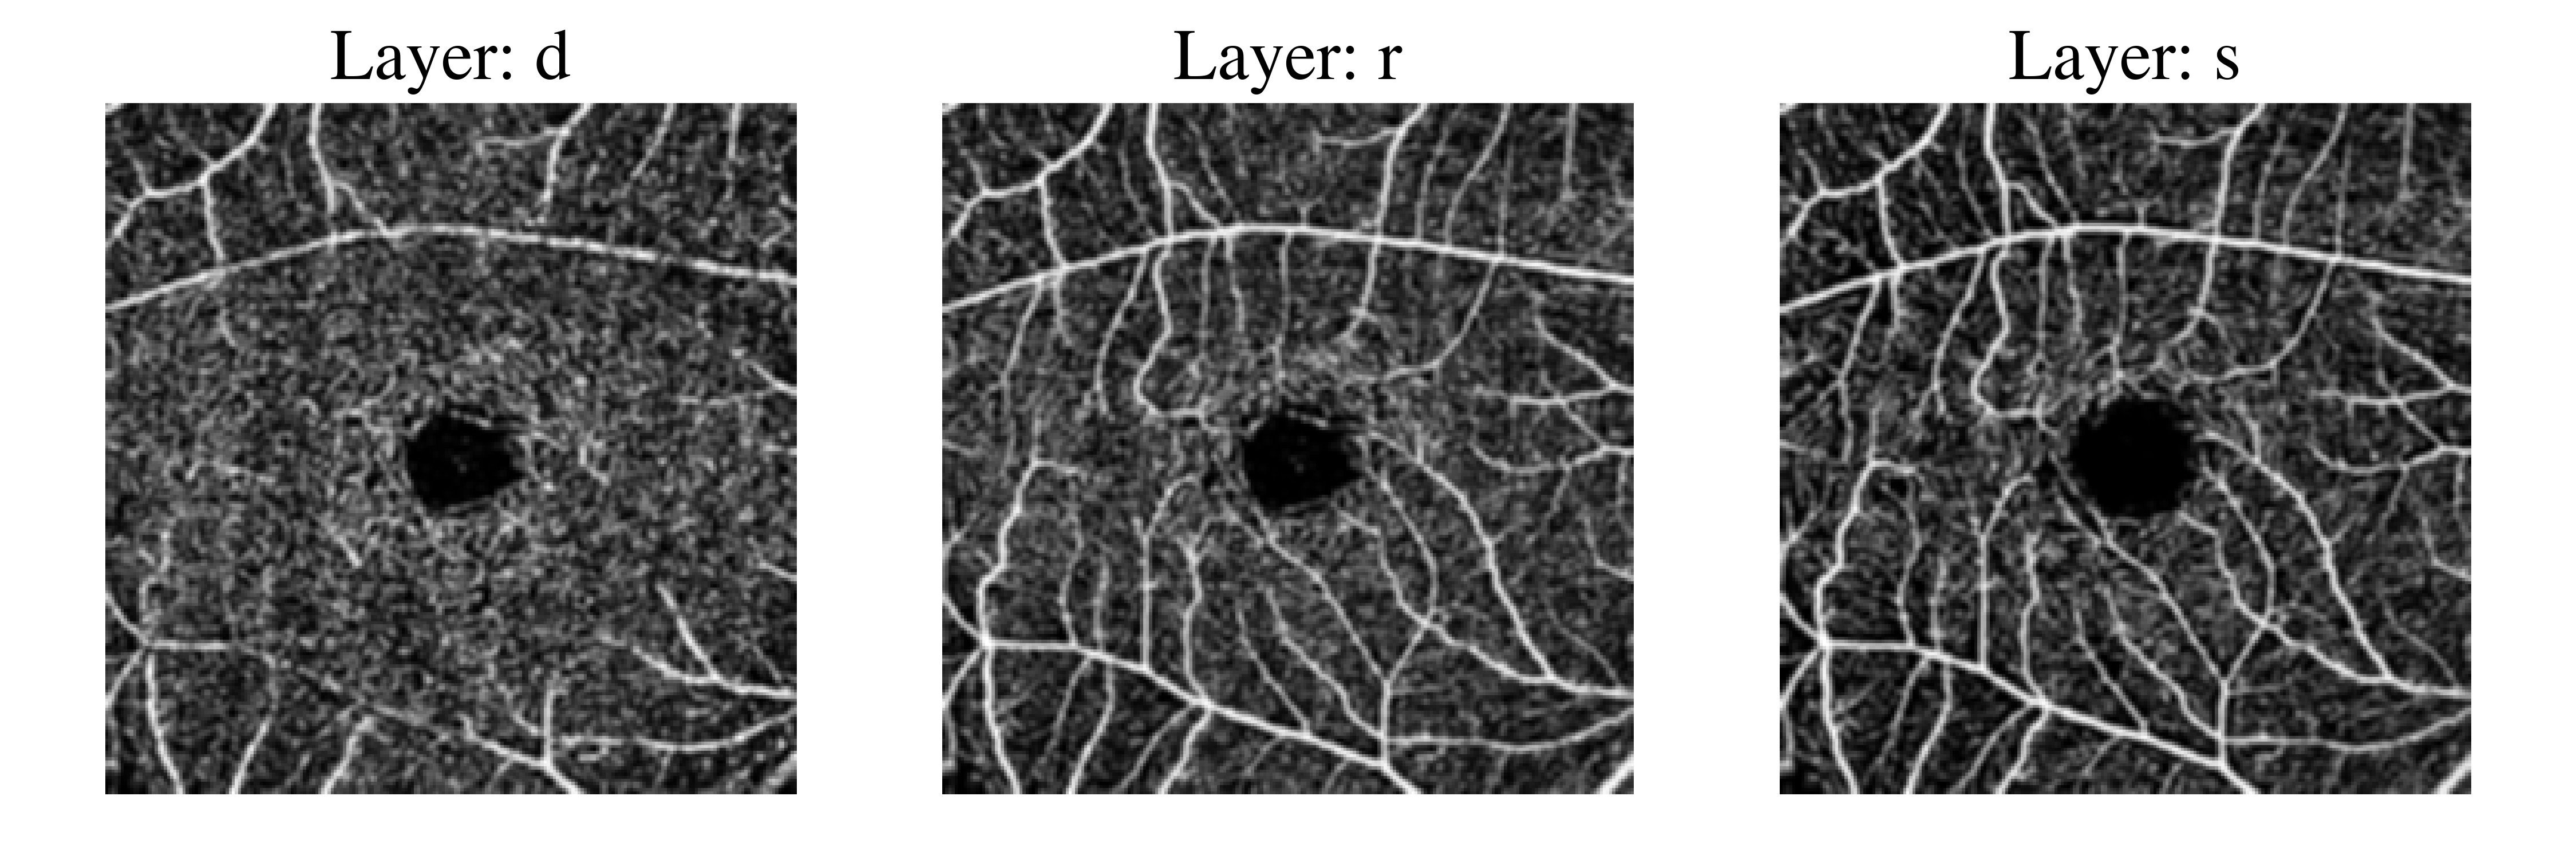
\includegraphics[width=300px]{../alld/plots/data_layers.png}
\end{center}
\caption{These 4 images illustrate the 4 layers of OCTA images in each sample after preprocessing. Retina d, o, r, s, represent deep, outer retina, choriocapillaries and superficial.}
\label{fig:layer-images}
\end{figure}


\subsection{Model Architecture}
Due to the limited data used in this study, we applied transfer learning using models pretrained on the ImageNET dataset. Early stopping was used such that the best model saved was based on the lowest validation loss. All models were implemented using PyTorch.

\subsubsection{Vanilla Convolution Neural Network (CNN)}
The Vanilla CNN model consists of four convolution blocks, each convolution block consists of a convolution layer with kernel size three, stride one, padding one, followed by a ReLU layer, a max pooling layer with kernel size two, stride two. The convolution blocks are followed by a fully connected layer with 512 hidden units, followed by a ReLU layer and a sigmoid layer. The model was trained using binary cross entropy loss and Adam optimizer with learning rate 1e-5 and batch size 8.

\subsubsection{ResNet}
We used a ResNet model as the base model and added a fully connected layer and a sigmoid layer at the end of the model to serve as a baseline model for comparison. All models were trained using binary cross entropy loss and Adam optimizer with learning rate 1e-5 and batch size 8. All models were trained with the original ResNet parameters frozen for 5-10 epochs, then trained with all parameters for 5-10 epochs.

\subsubsection{VGGNet}
We used a VGGNet model as the base model and added an additional classifier consisting of a Dropout Layer, a Linear Layer, a ReLU Layer, another set of Dropout, Linear, ReLU, followed by a Linear Layer to a sigmoid layer. The model was trained using binary cross entropy loss,  Adam optimizer with learning rate 1e-5 and batch size 8. The VGG16 model was trained with the original VGG16 parameters frozen for 5 epochs, then trained with all parameters for 5 epochs. The VGG19 model was trained with the original VGG19 parameters frozen for 10 epochs, then trained with all parameters for 2 epochs.

\section{Results}
The model was first trained and evaluated on different layers of the OCTA images to understand which layers may be most informative. The data was trained using a Vanilla CNN and a pretrained ResNet18 and ResNet50. The test results are shown in Table~\ref{model-evaluation-table-random} and the training results are shown in Figure~\ref{fig:resnet18-random}. Both ResNET models are able to outperform the Vanilla CNN, which indicates that transfer learning may be beneficial in this scenario. The performance of ResNet18 is better than ResNet50, which is likely due to overfitting. The performance of ResNet18 and ResNet50 both exceed the results from \citet{WISELY2024100355}, likely because the dataset used in this study is larger and better balanced.

\begin{figure}[h]
   \begin{center}
   \label{fig:resnet18-random}
   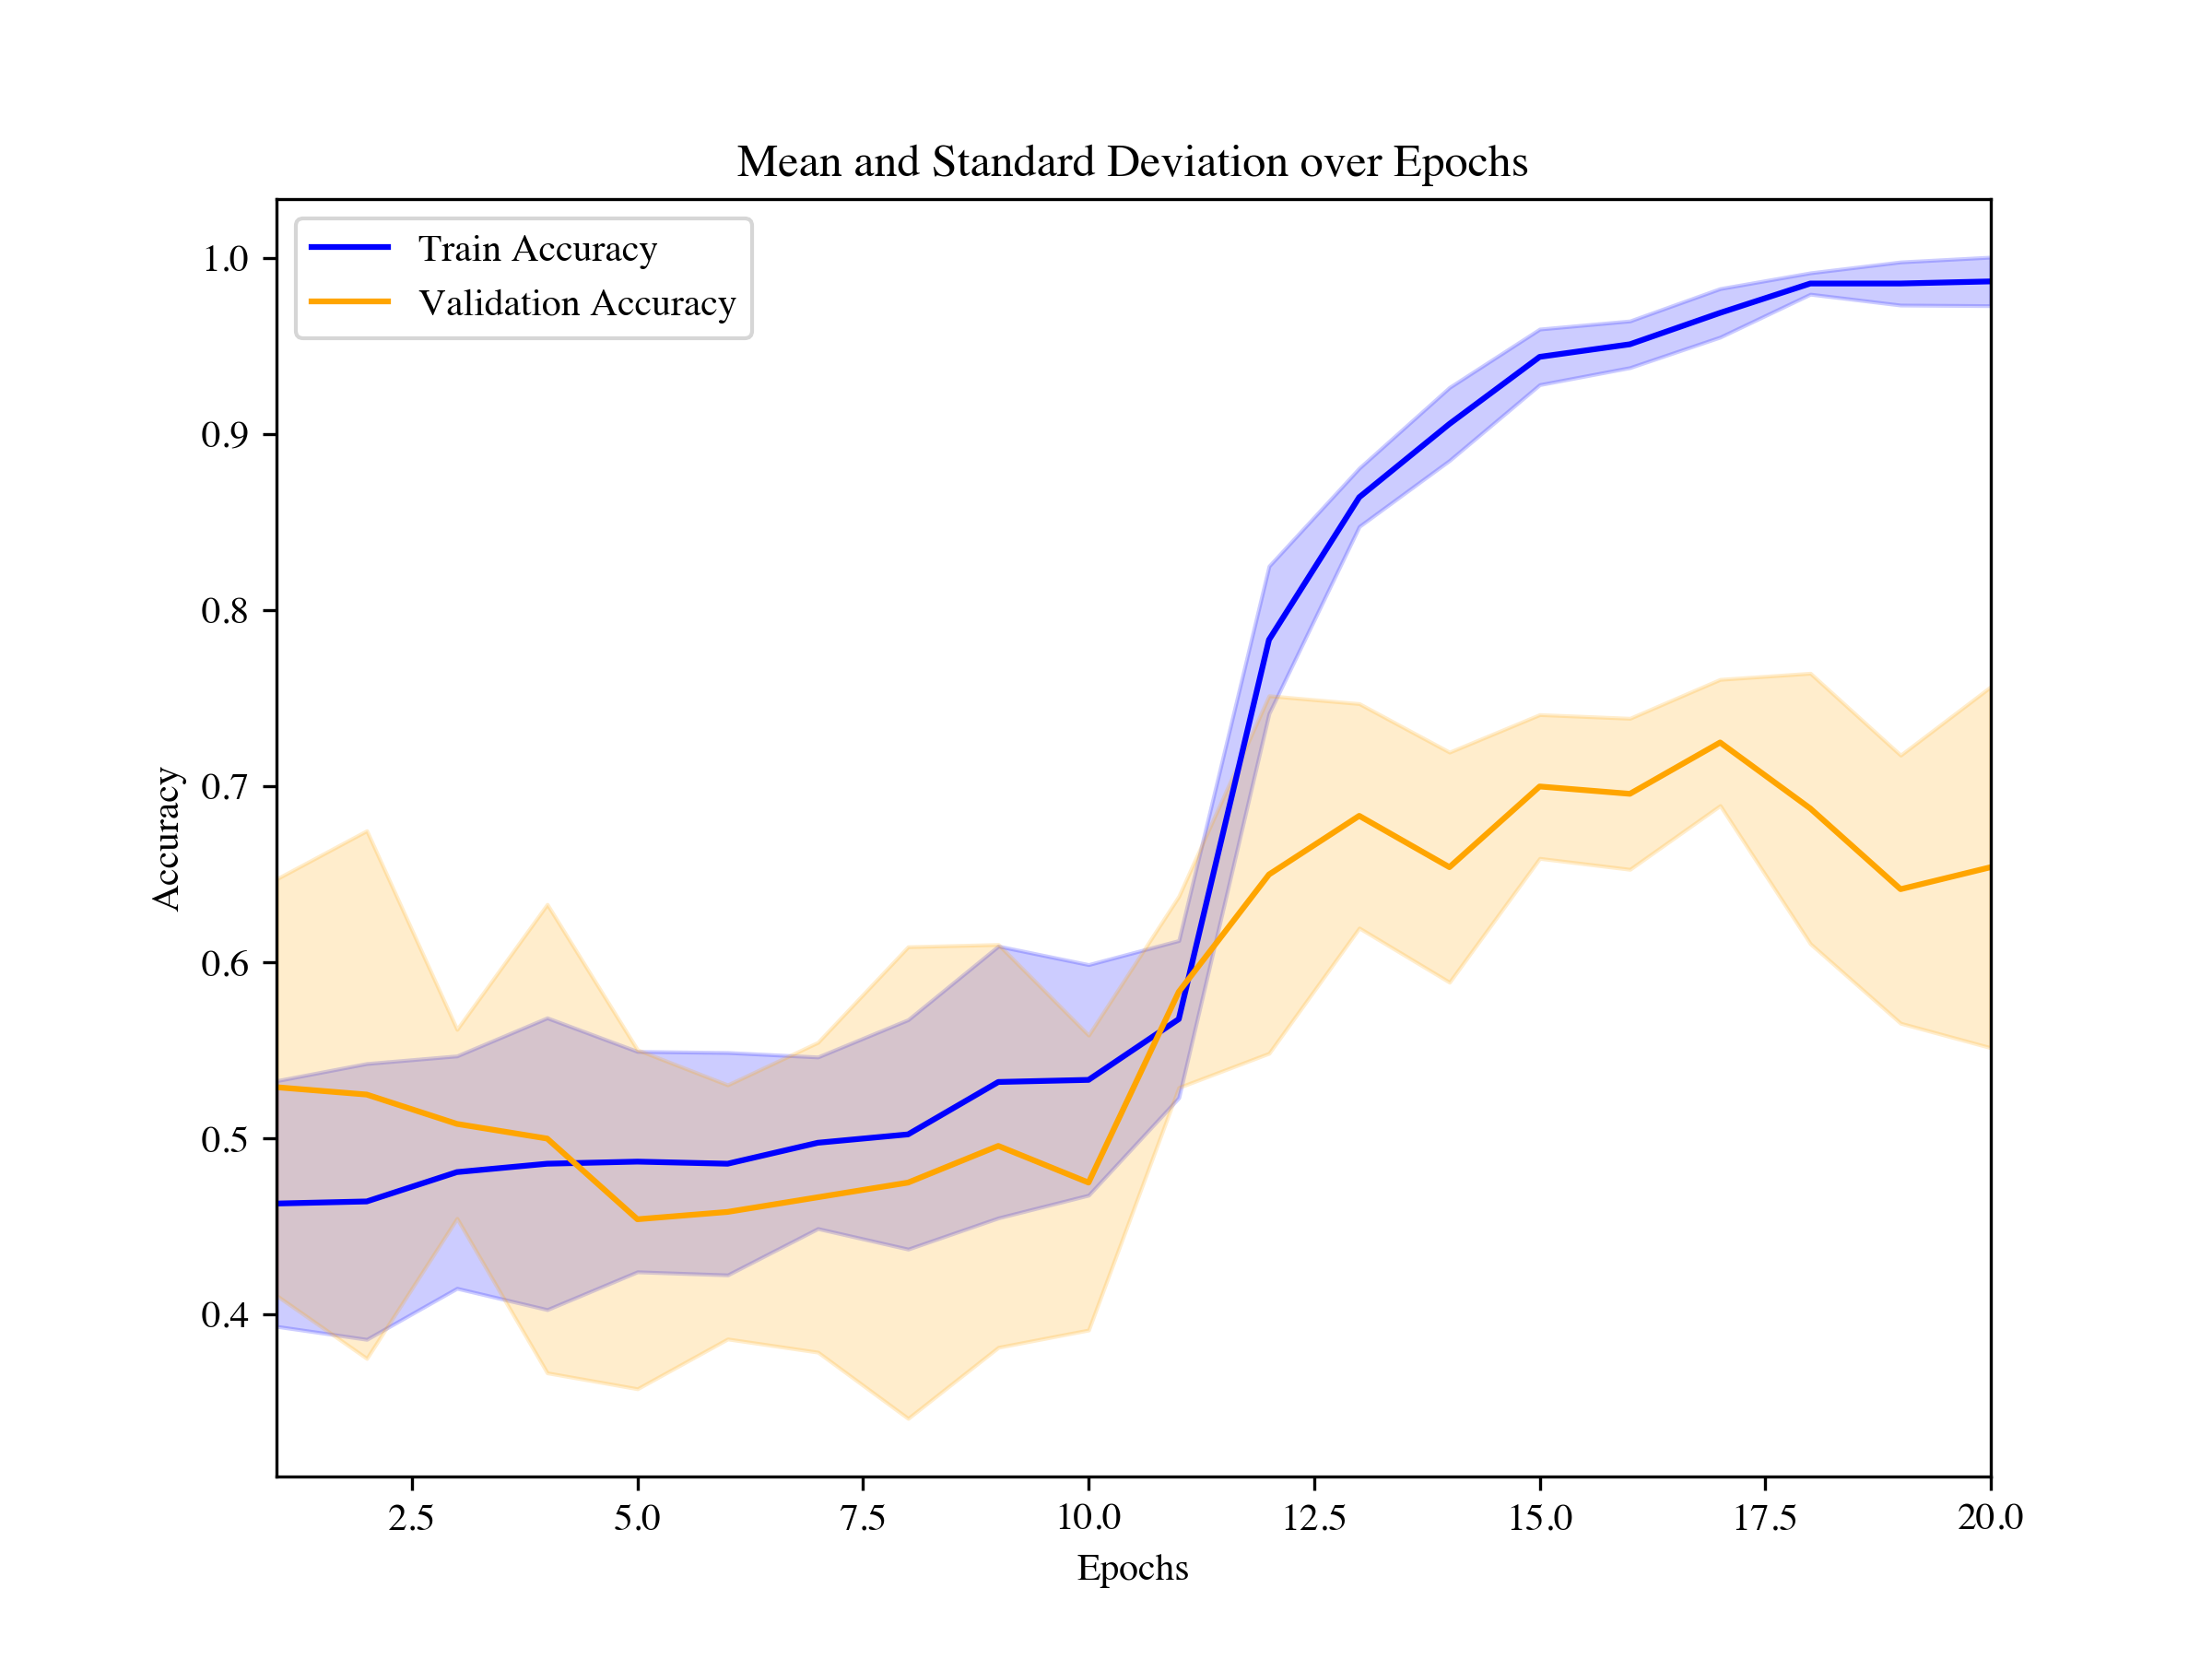
\includegraphics[width=.30\linewidth]{../plots/resnet18/accuracy.png}
   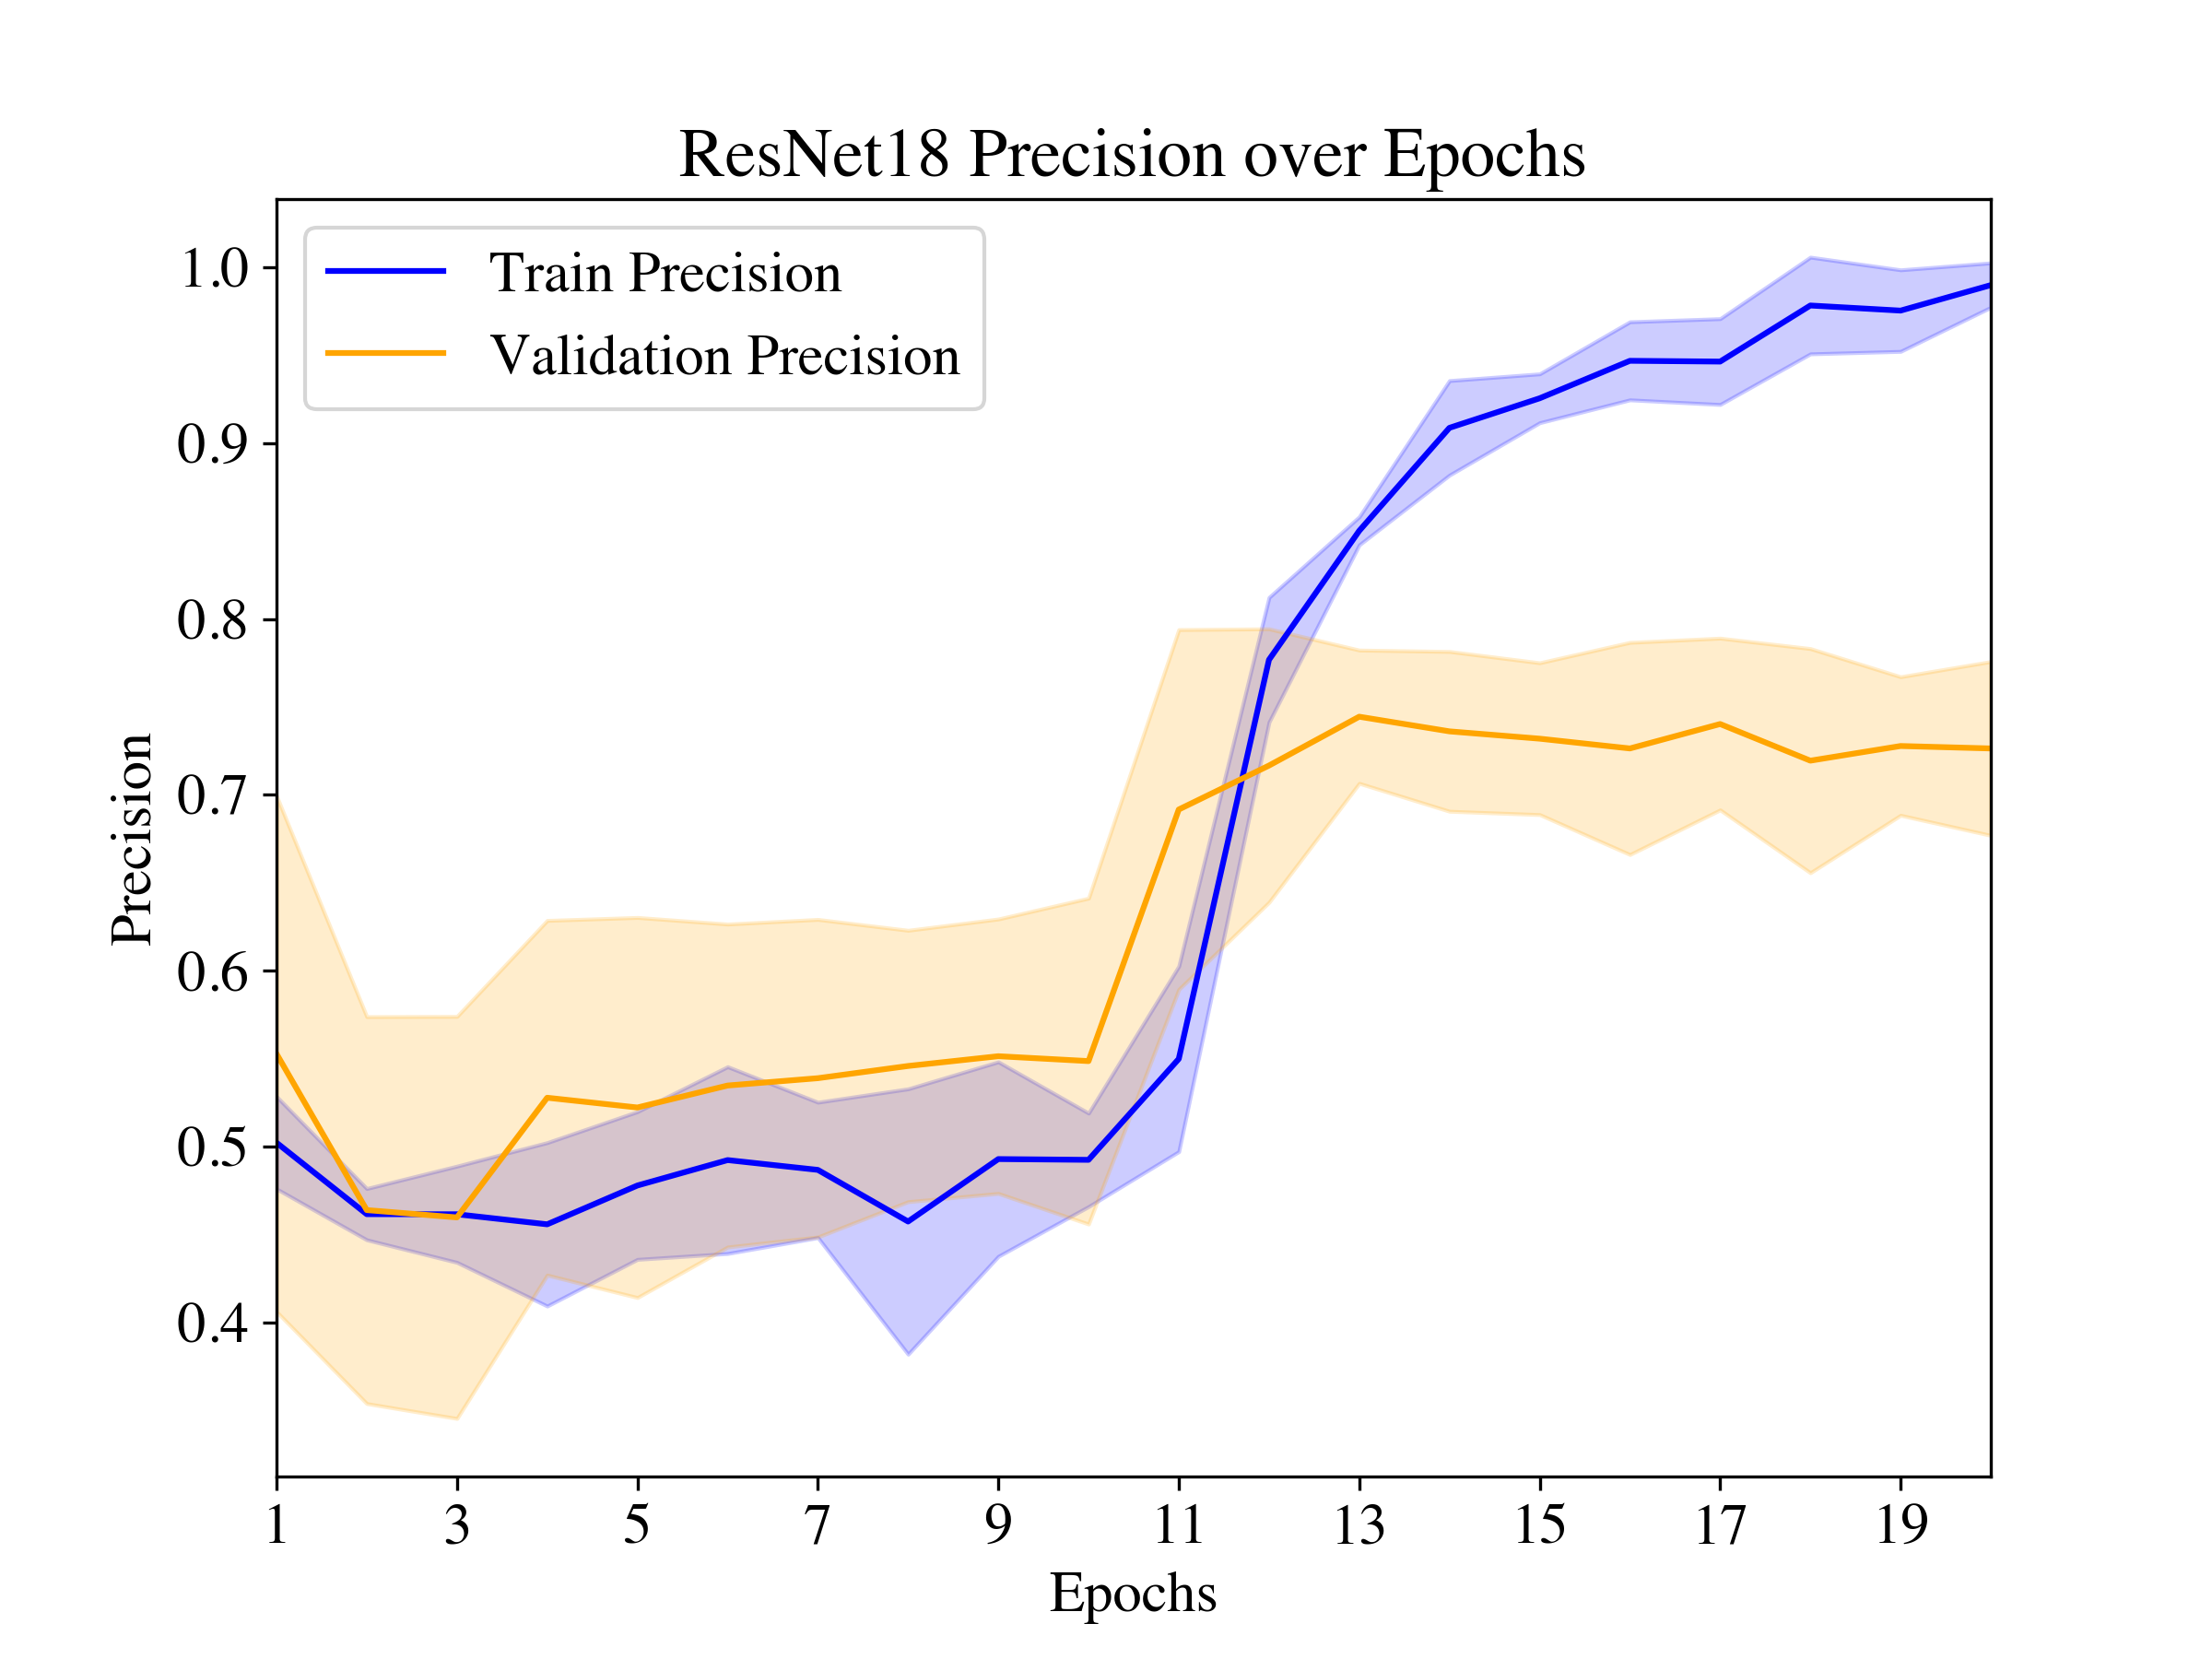
\includegraphics[width=.30\linewidth]{../plots/resnet18/precision.png}
   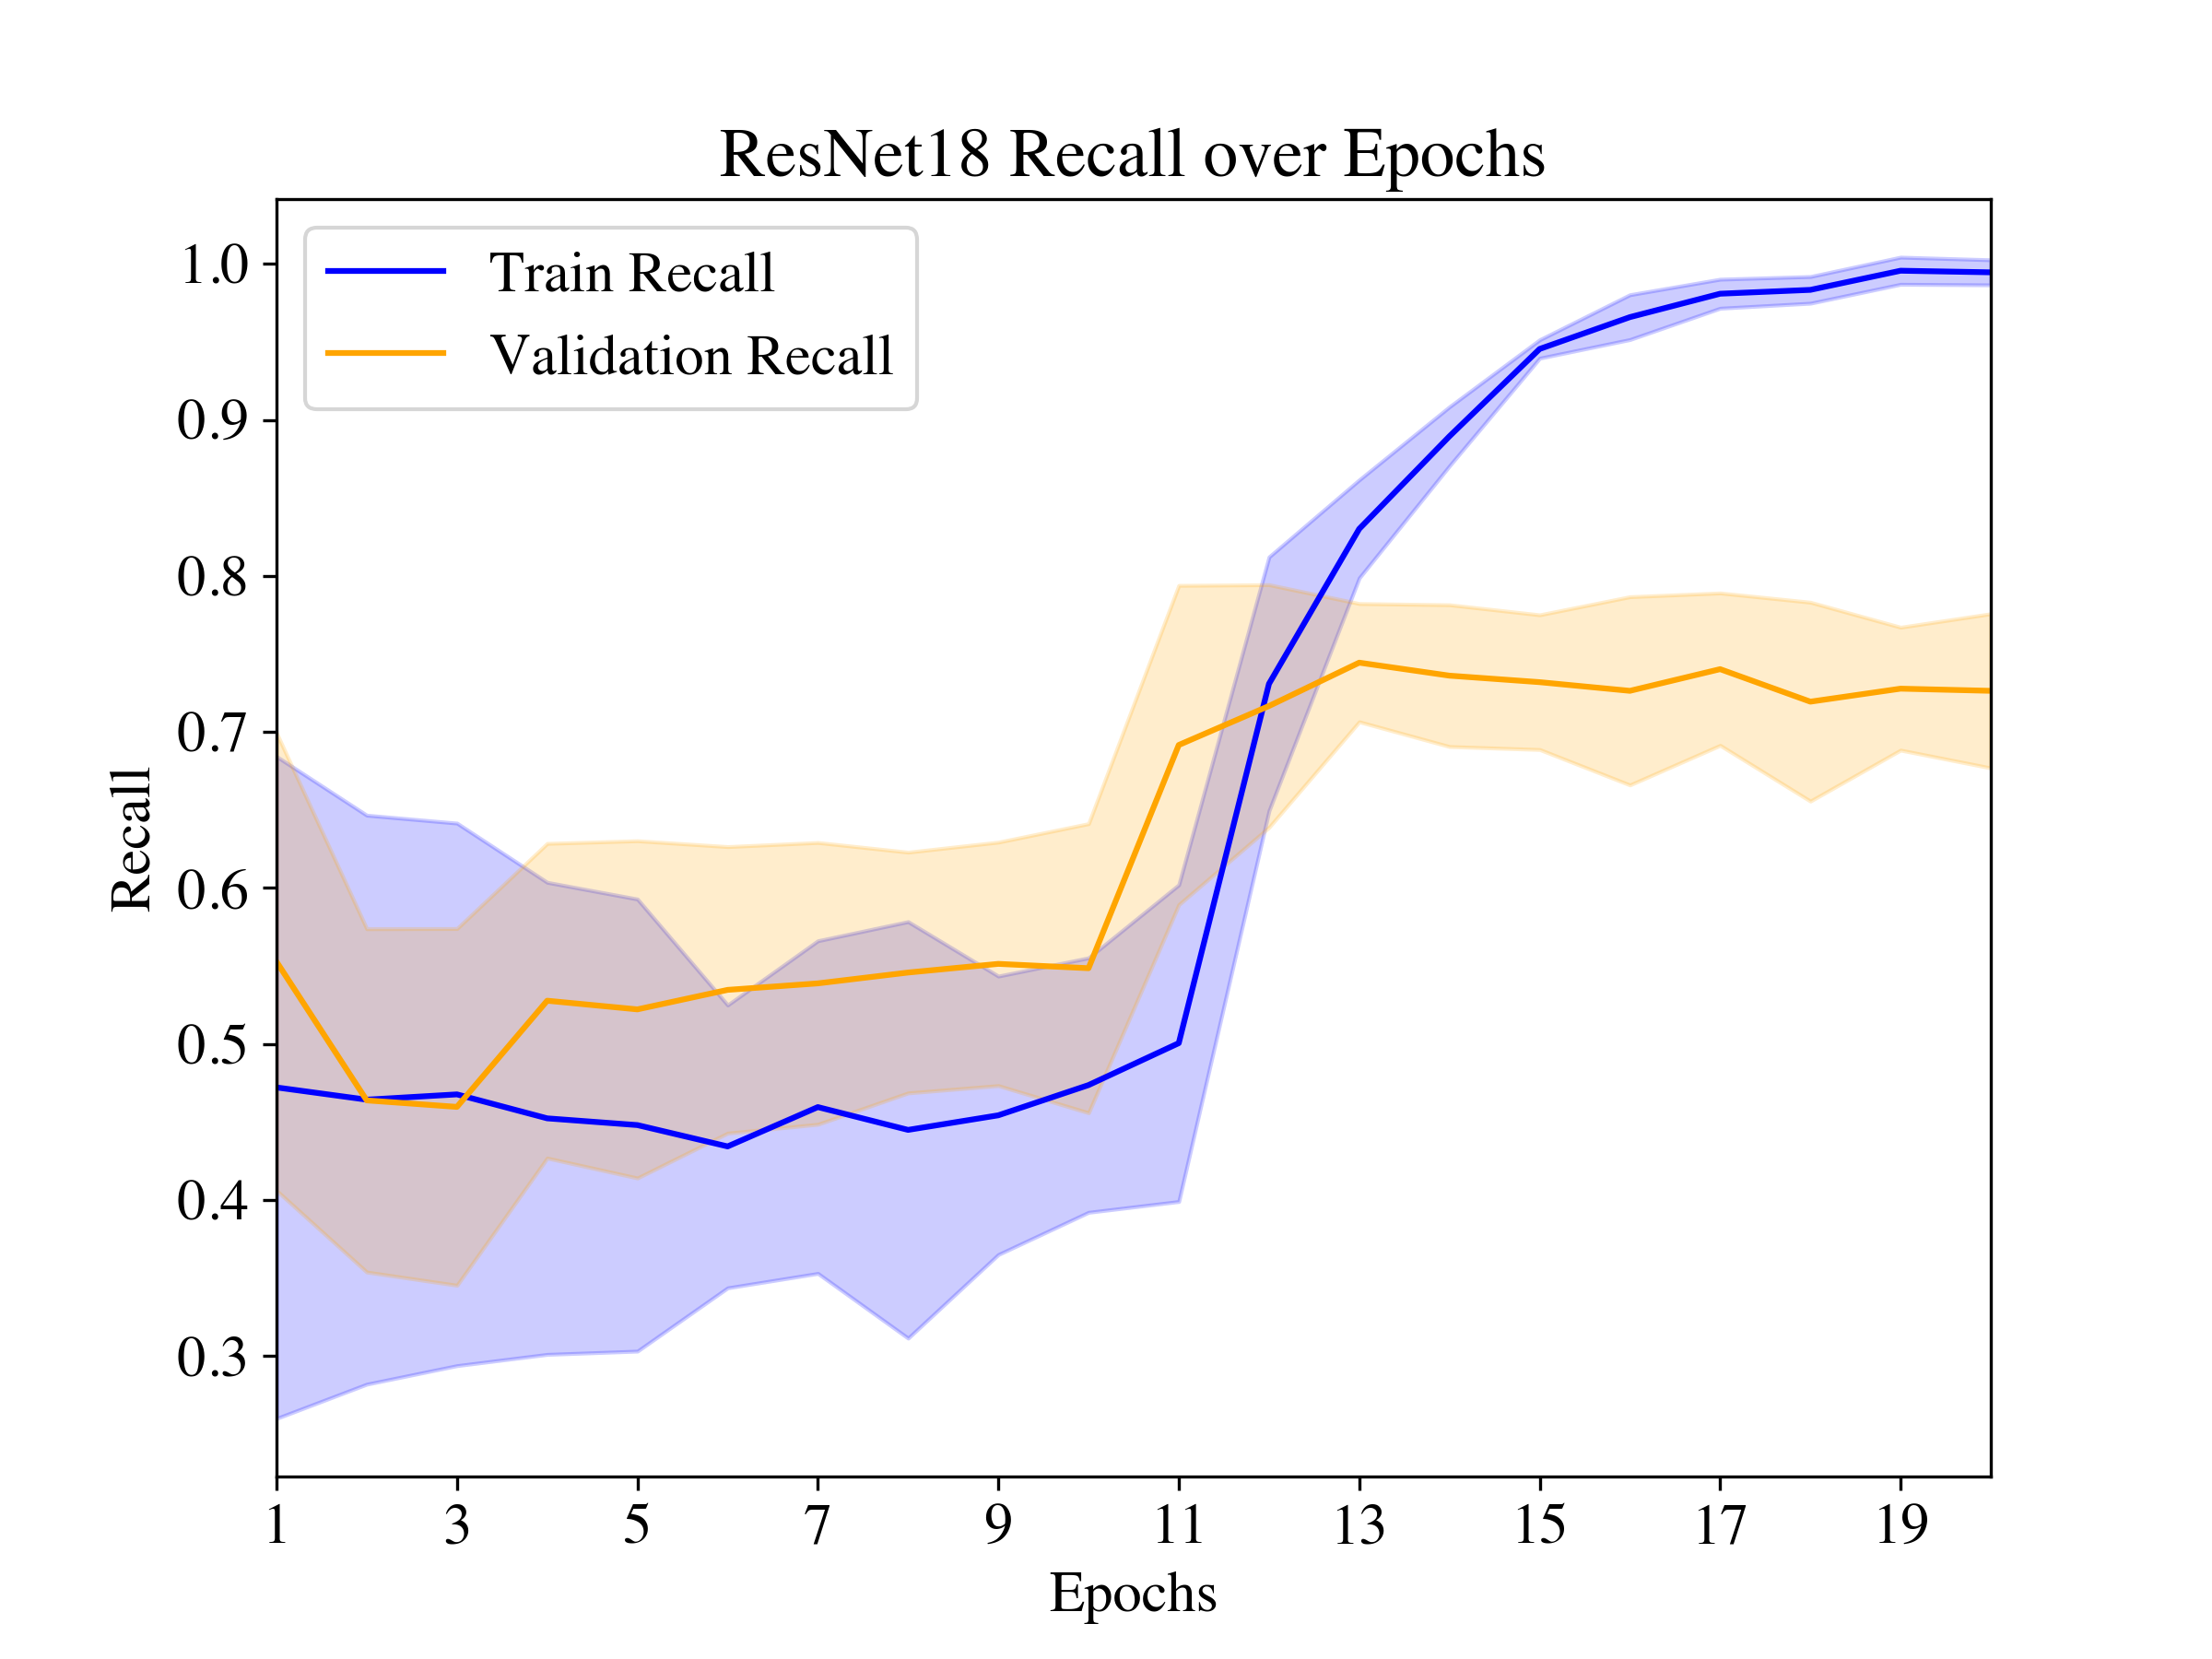
\includegraphics[width=.30\linewidth]{../plots/resnet18/recall.png}
   \end{center}
   \caption{ResNet18 train (blue) and validation (orange) accuracy curve (left) precision curve (center) and recall curve (right) with mean and standard deviation. This model was trained only on the Retina Layer R.}
   \end{figure}

\begin{table}[h]
   \caption{Comparison of VanillaCNN, ResNet18 and ResNet50 when trained on different layers of the OCTA image. All values are evaluated on the test set using five-fold Cross Validation. ACC is accuracy, Precision is precision score, Recall is recall score, F1 is F1 score, AUC is area under the receiver operating characteristic (ROC) curve.}
   \label{model-evaluation-table-random}
   \begin{center}
   \begin{tabular}{llllll}
   \multicolumn{1}{c}{\bf Model}  &\multicolumn{1}{c}{\bf ACC} &\multicolumn{1}{c}{\bf Precision} &\multicolumn{1}{c}{\bf Recall} &\multicolumn{1}{c}{\bf F1} &\multicolumn{1}{c}{\bf AUC}
   \\ \hline \\
   \bf Layer R\\
   VanillaCNN        &$0.59\pm0.01$ &$0.61\pm0.03$ &$0.31\pm0.05$ &$0.41\pm0.04$ &$0.56\pm0.01$\\
   ResNet18         &$0.67\pm0.03$ &$0.67\pm0.03$ &$0.59\pm0.06$ &$0.62\pm0.05$ &$\mathbf{0.67\pm0.03}$\\
   ResNet50         &$0.63\pm0.04$ &$0.63\pm0.06$ &$0.54\pm0.13$ &$0.56\pm0.08$ &$0.62\pm0.04$\\
   \\ \hline \\
   \bf Layer D\\
   VanillaCNN &$0.57\pm0.06$ &$0.56\pm0.12$ &$0.36\pm0.14$ &$0.42\pm0.12$ &$0.56\pm0.06$\\
   ResNet18   &$0.65\pm0.06$ &$0.65\pm0.08$ &$0.51\pm0.14$ &$0.56\pm0.11$ &$0.64\pm0.06$\\
   ResNet50   &$0.67\pm0.06$ &$0.68\pm0.10$ &$0.57\pm0.12$ &$0.61\pm0.08$ &$\mathbf{0.66\pm0.06}$\\
   \\ \hline \\
   \bf Layer O\\
   VanillaCNN &$0.59\pm0.08$ &$0.60\pm0.07$ &$0.91\pm0.09$ &$0.72\pm0.05$ &$0.53\pm0.06$\\
   ResNet18 &$0.65\pm0.07$ &$0.71\pm0.10$ &$0.67\pm0.12$ &$0.68\pm0.09$ &$\mathbf{0.65\pm0.06}$\\
   ResNet50 &$0.61\pm0.09$ &$0.65\pm0.08$ &$0.65\pm0.12$ &$0.64\pm0.10$ &$0.59\pm0.09$\\
   \\ \hline \\
   \bf Layer S\\
   VanillaCNN &$0.62\pm0.01$ &$0.68\pm0.05$ &$0.36\pm0.10$ &$0.46\pm0.09$ &$0.61\pm0.02$\\
   ResNet18 &$0.66\pm0.03$ &$0.68\pm0.07$ &$0.50\pm0.10$ &$0.56\pm0.07$ &$\mathbf{0.65\pm0.03}$\\
   ResNet50 &$0.65\pm0.03$ &$0.65\pm0.06$ &$0.56\pm0.11$ &$0.58\pm0.07$ &${0.65\pm0.02}$\\
   \end{tabular}
   \end{center}
\end{table}

\begin{table}[h]
   \caption{Comparison of VanillaCNN, ResNet18 and ResNet50 when trained on concatenated R, D, S layers of the OCTA image. All values are evaluated on the test set using five-fold Cross Validation. ACC is accuracy, Precision is precision score, Recall is recall score, F1 is F1 score, AUC is area under the ROC curve.}
   \label{model-evaluation-table}
   \begin{center}
   \begin{tabular}{llllll}
   \multicolumn{1}{c}{\bf Model}  &\multicolumn{1}{c}{\bf ACC} &\multicolumn{1}{c}{\bf Precision} &\multicolumn{1}{c}{\bf Recall} &\multicolumn{1}{c}{\bf F1} &\multicolumn{1}{c}{\bf AUC}
   \\ \hline \\
   VanillaCNN       &$0.63\pm0.06$ &$0.71\pm0.11$ &$0.37\pm0.15$ &$0.45\pm0.14$ &$0.61\pm0.07$\\
   ResNet18         &$0.68\pm0.07$ &$0.68\pm0.09$ &$0.58\pm0.15$ &$0.62\pm0.11$ &$0.67\pm0.08$\\
   ResNet50         &$0.67\pm0.06$ &$0.64\pm0.08$ &$0.60\pm0.14$ &$0.61\pm0.10$ &$0.67\pm0.05$\\
   VGG16            &$0.69\pm0.04$ &$0.73\pm0.06$ &$0.53\pm0.10$ &$0.60\pm0.08$ &$0.67\pm0.05$\\
   VGG19            &$0.65\pm0.05$ &$0.66\pm0.05$ &$0.49\pm0.17$ &$0.55\pm0.11$ &$0.64\pm0.05$\\
   \end{tabular}
   \end{center}
   \end{table}

From Table~\ref{model-evaluation-table-random}, we noticed that the performance was better on layers R, D and S. Thus, we further trained the model by concatentating all 3 layers of OCTA images. Table~\ref{model-evaluation-table} shows the results from each of the models when trained on data from all 3 layers of OCTA images. ResNet18 shows the best performance among all the models. The performance of ResNet50 is worse than ResNet18, which is likely due to overfitting. The performance of VGG16 and VGG19 are similar, with VGG16 performing slightly better. The performance did not significantly improve compared to using only one layer. This may be due to the fact that each layer's feature is different, and concatenating the layers may not be the best way to combine the features. Future work includes using a weighted average from the results, or first doing feature extraction on each layer, then concatenating the features.

\begin{figure}[h]
\begin{center}
\label{fig:resnet18-3layer}
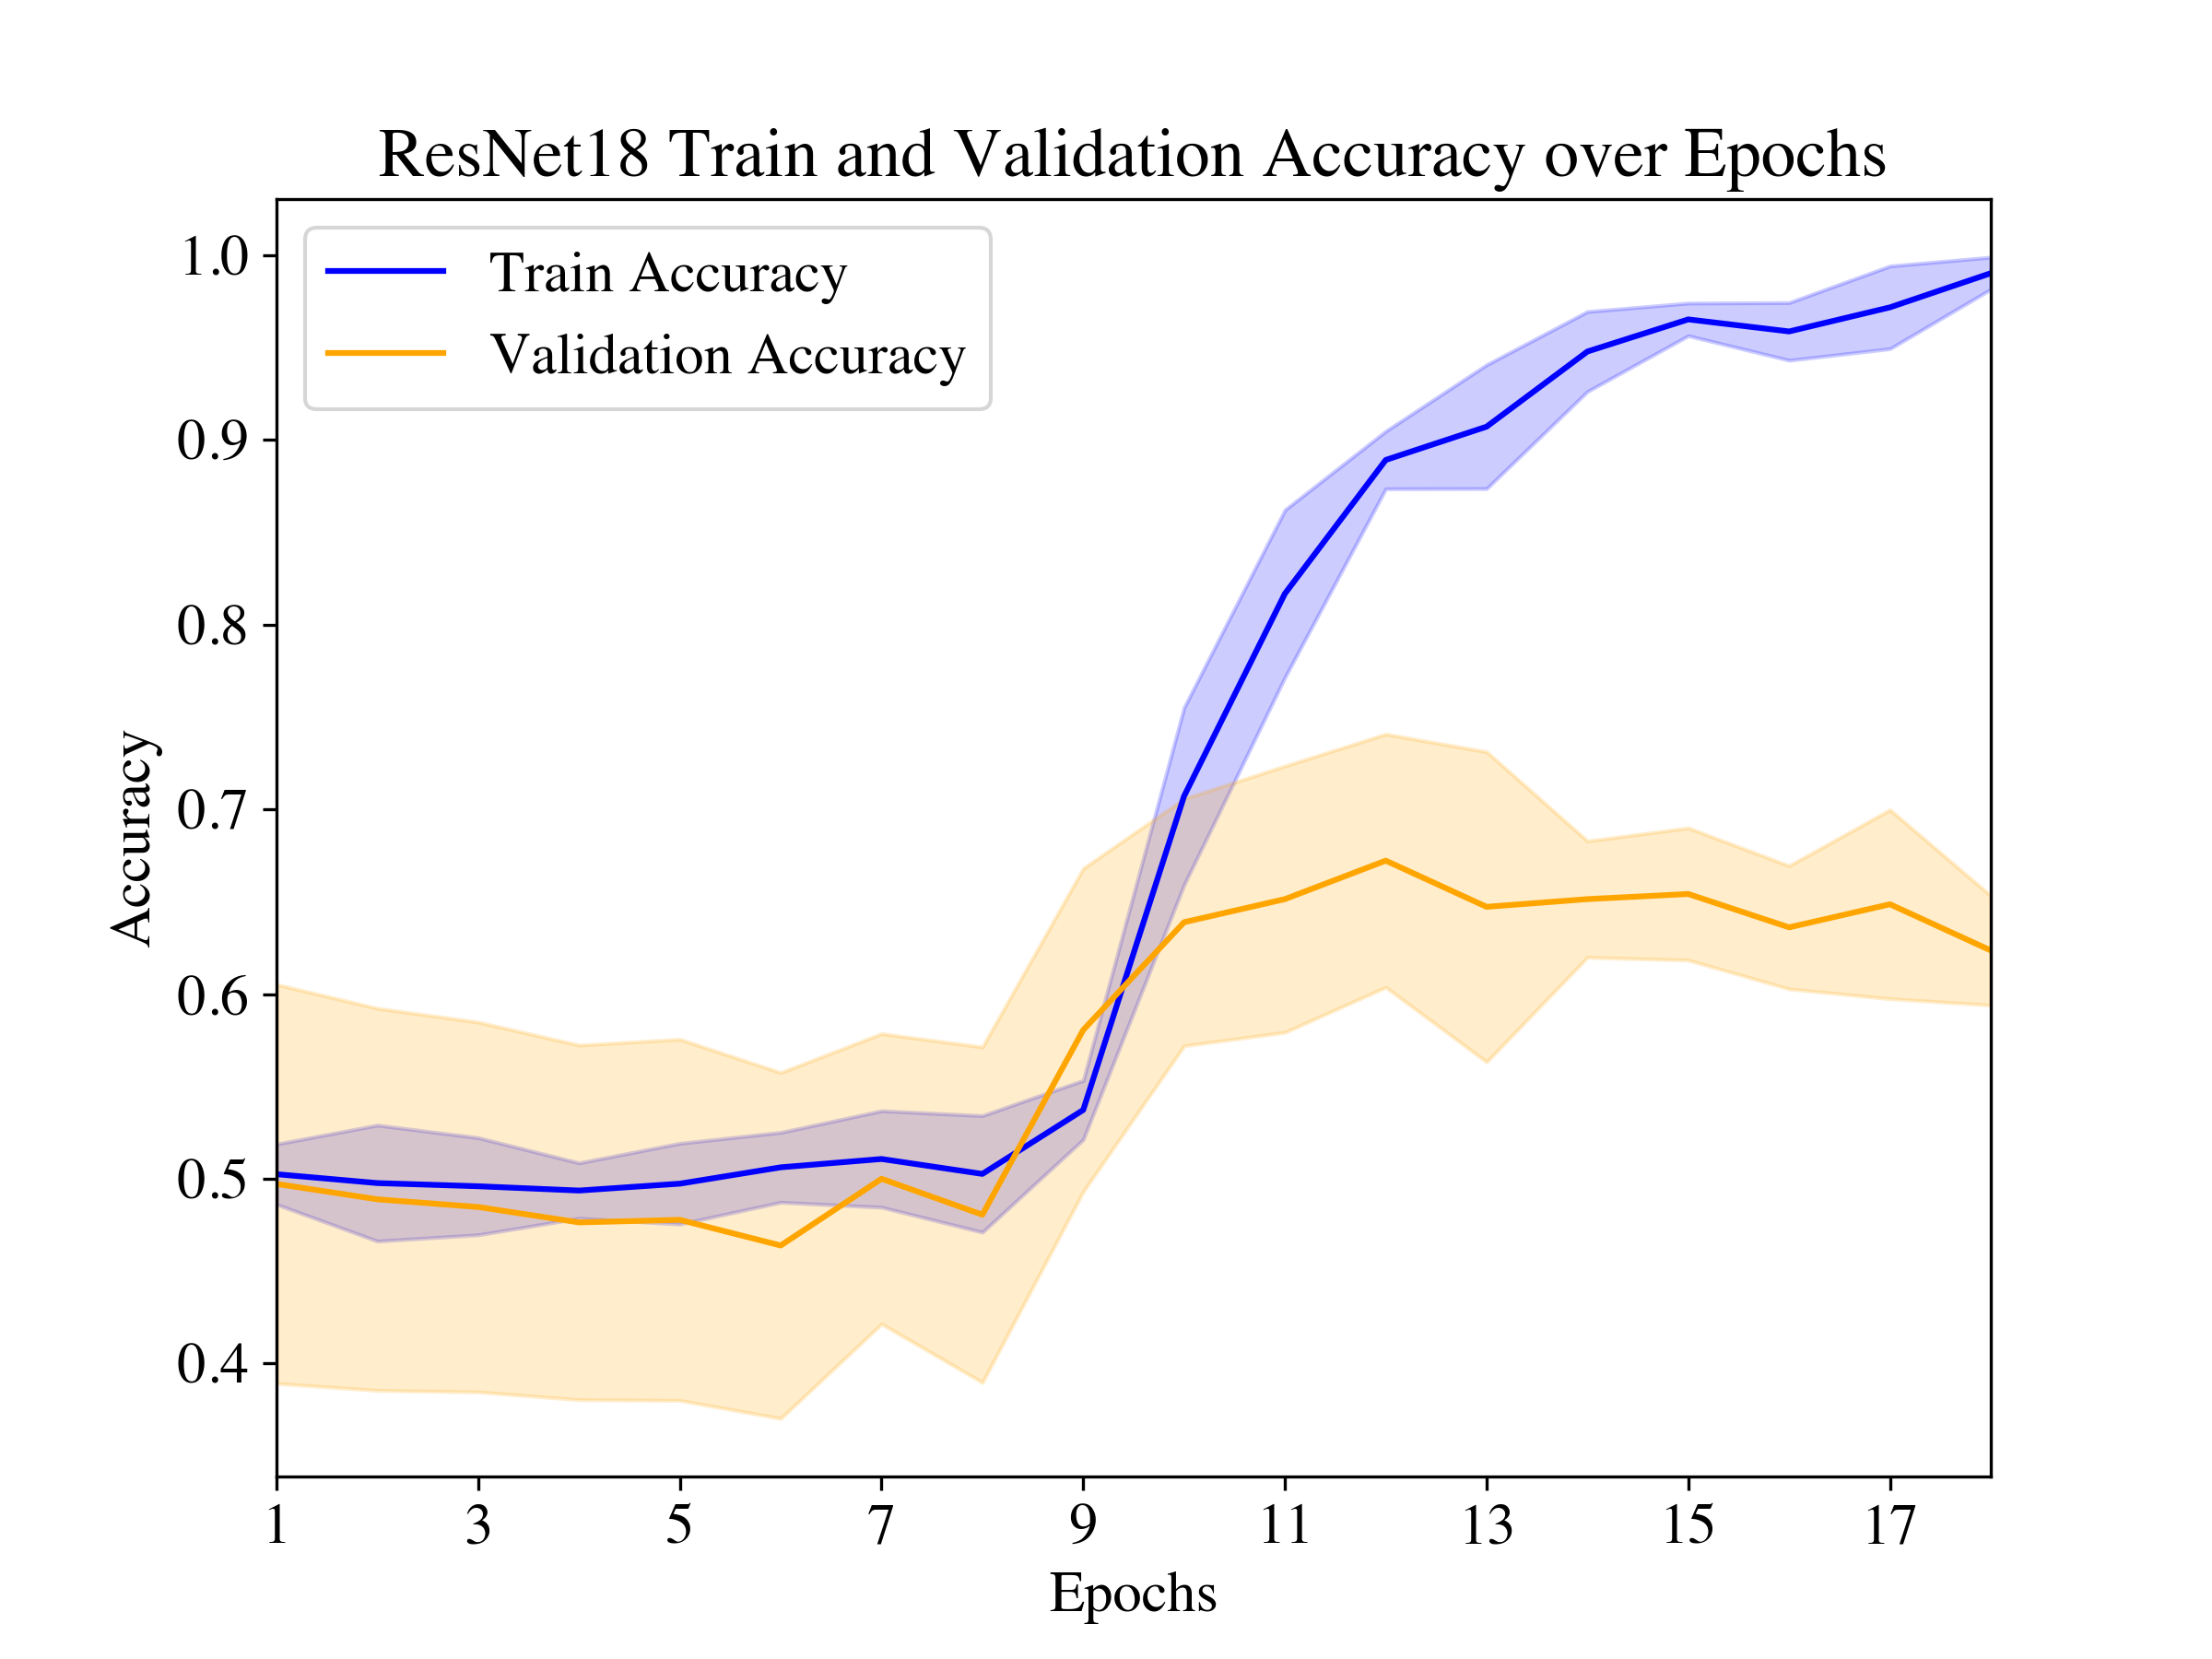
\includegraphics[width=.30\linewidth]{../3d/plots/resnet18/accuracy.png}
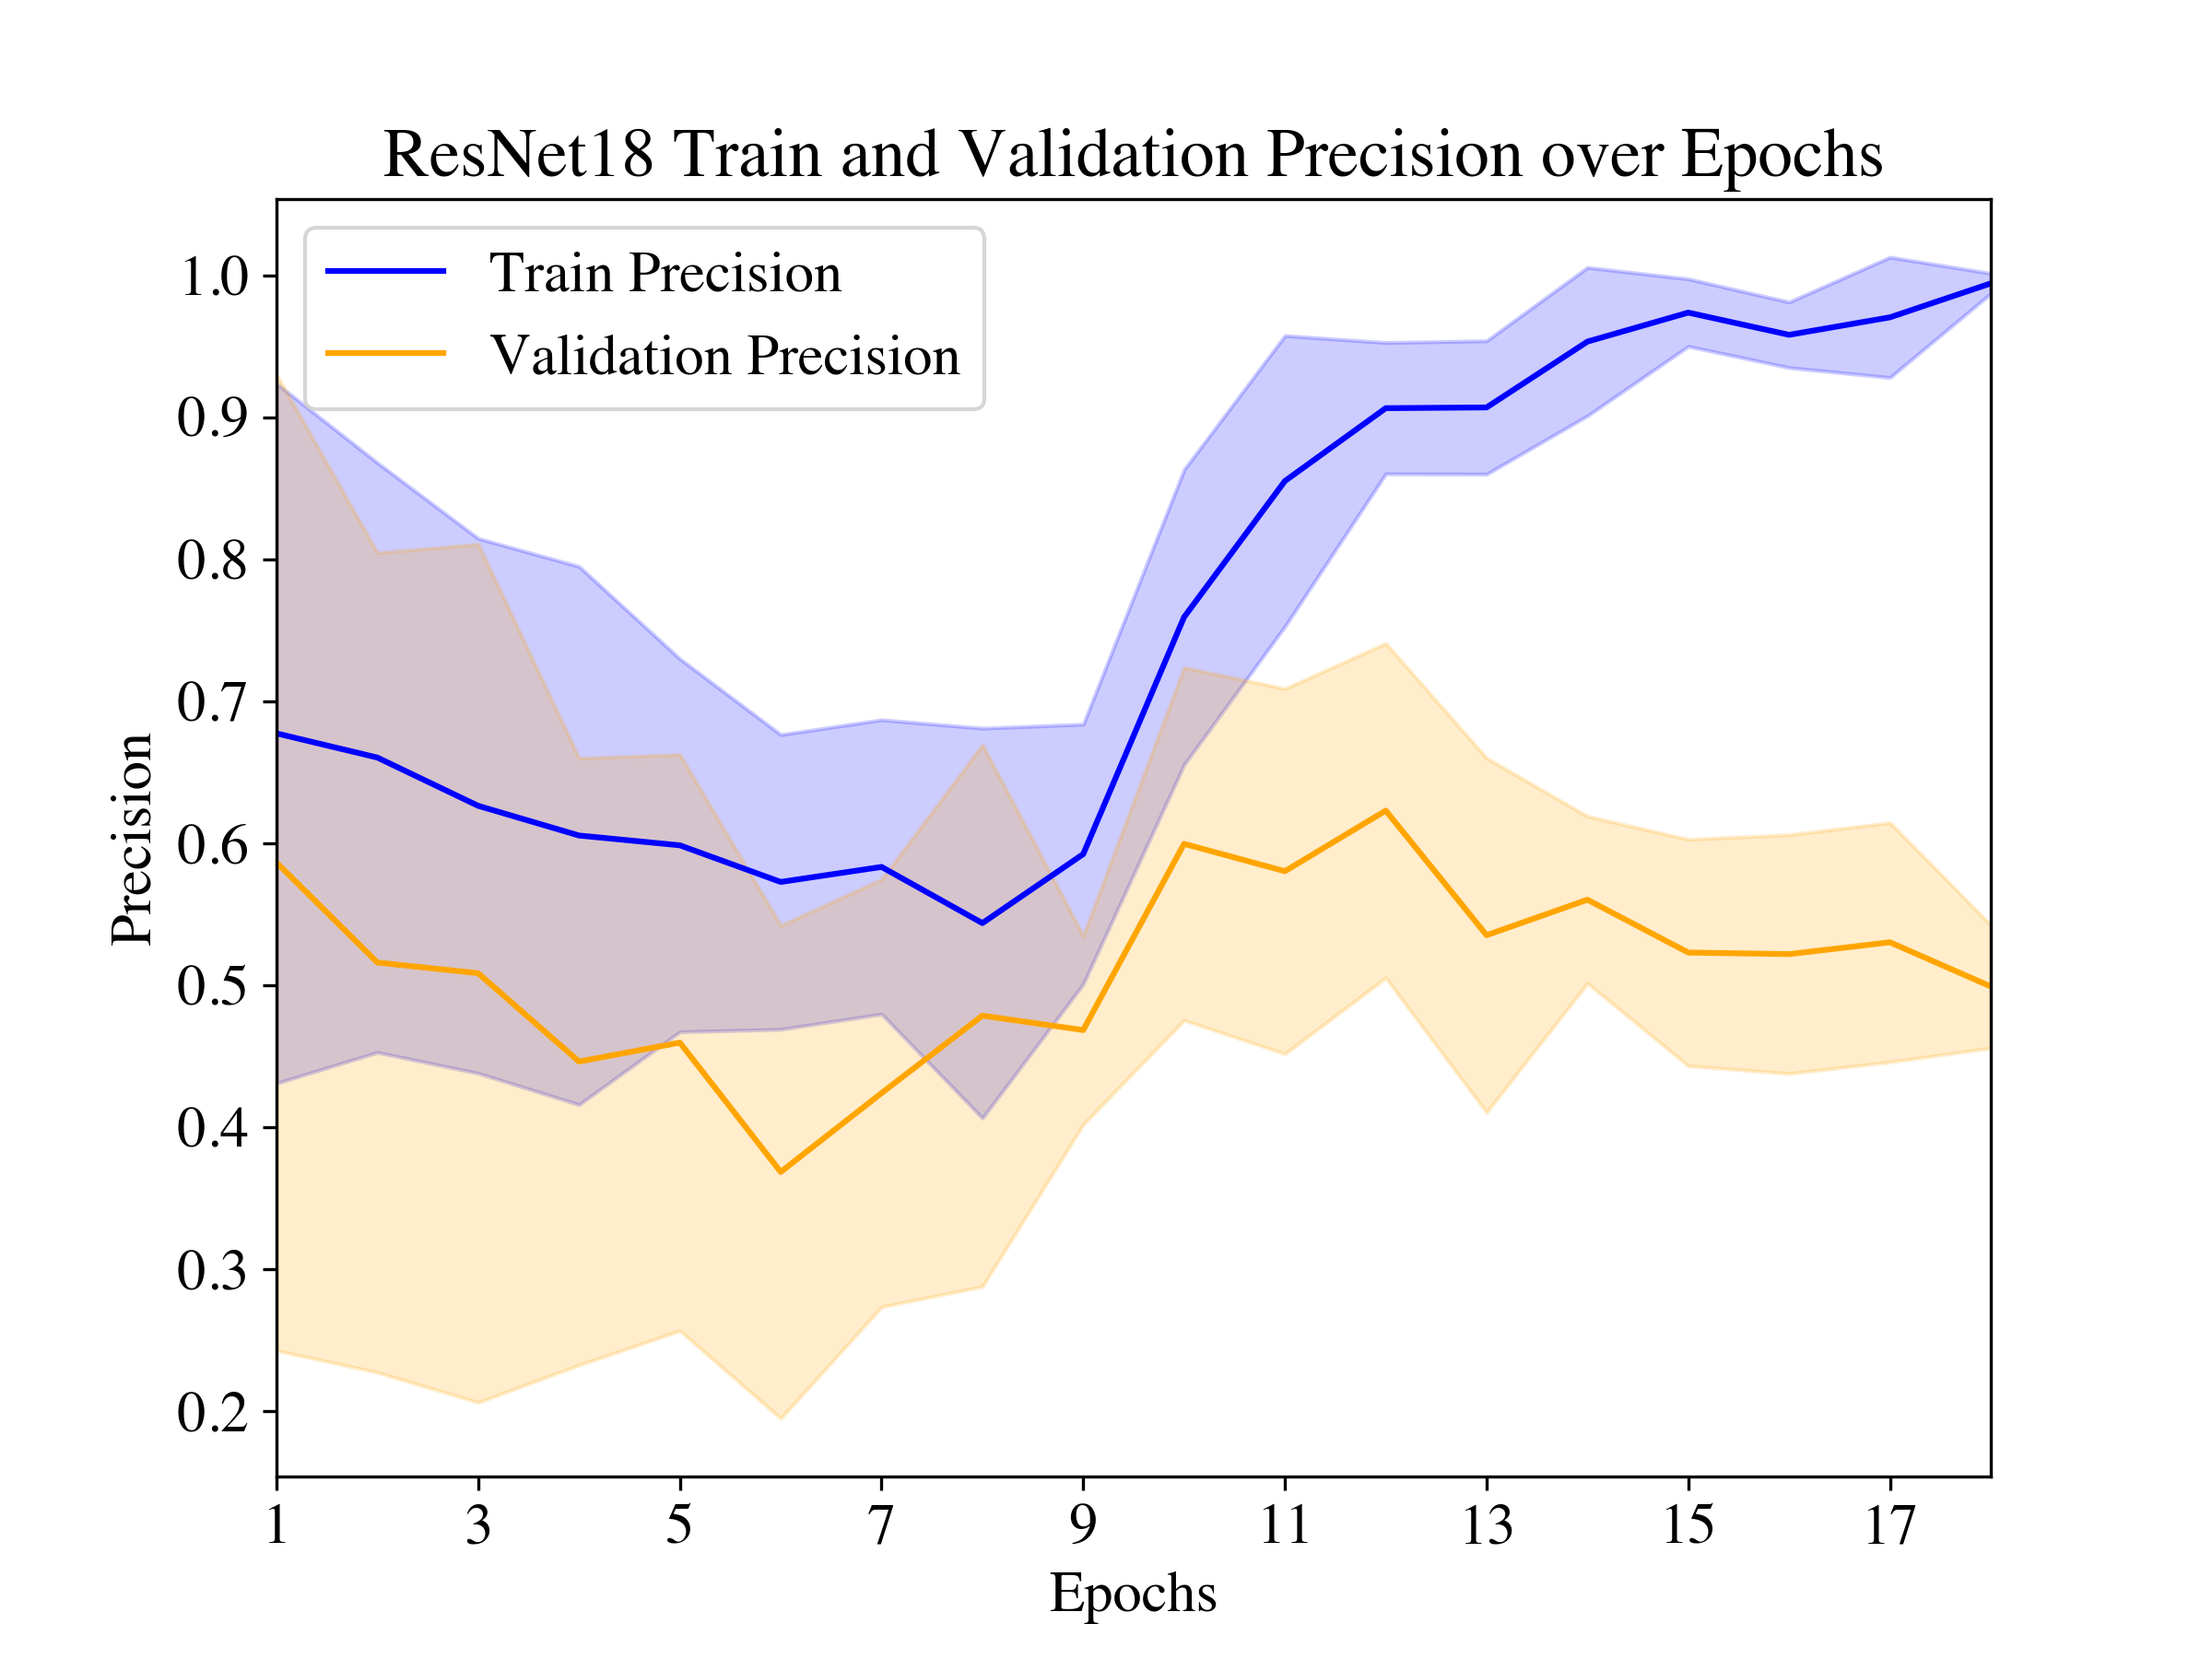
\includegraphics[width=.30\linewidth]{../3d/plots/resnet18/precision_score.png}
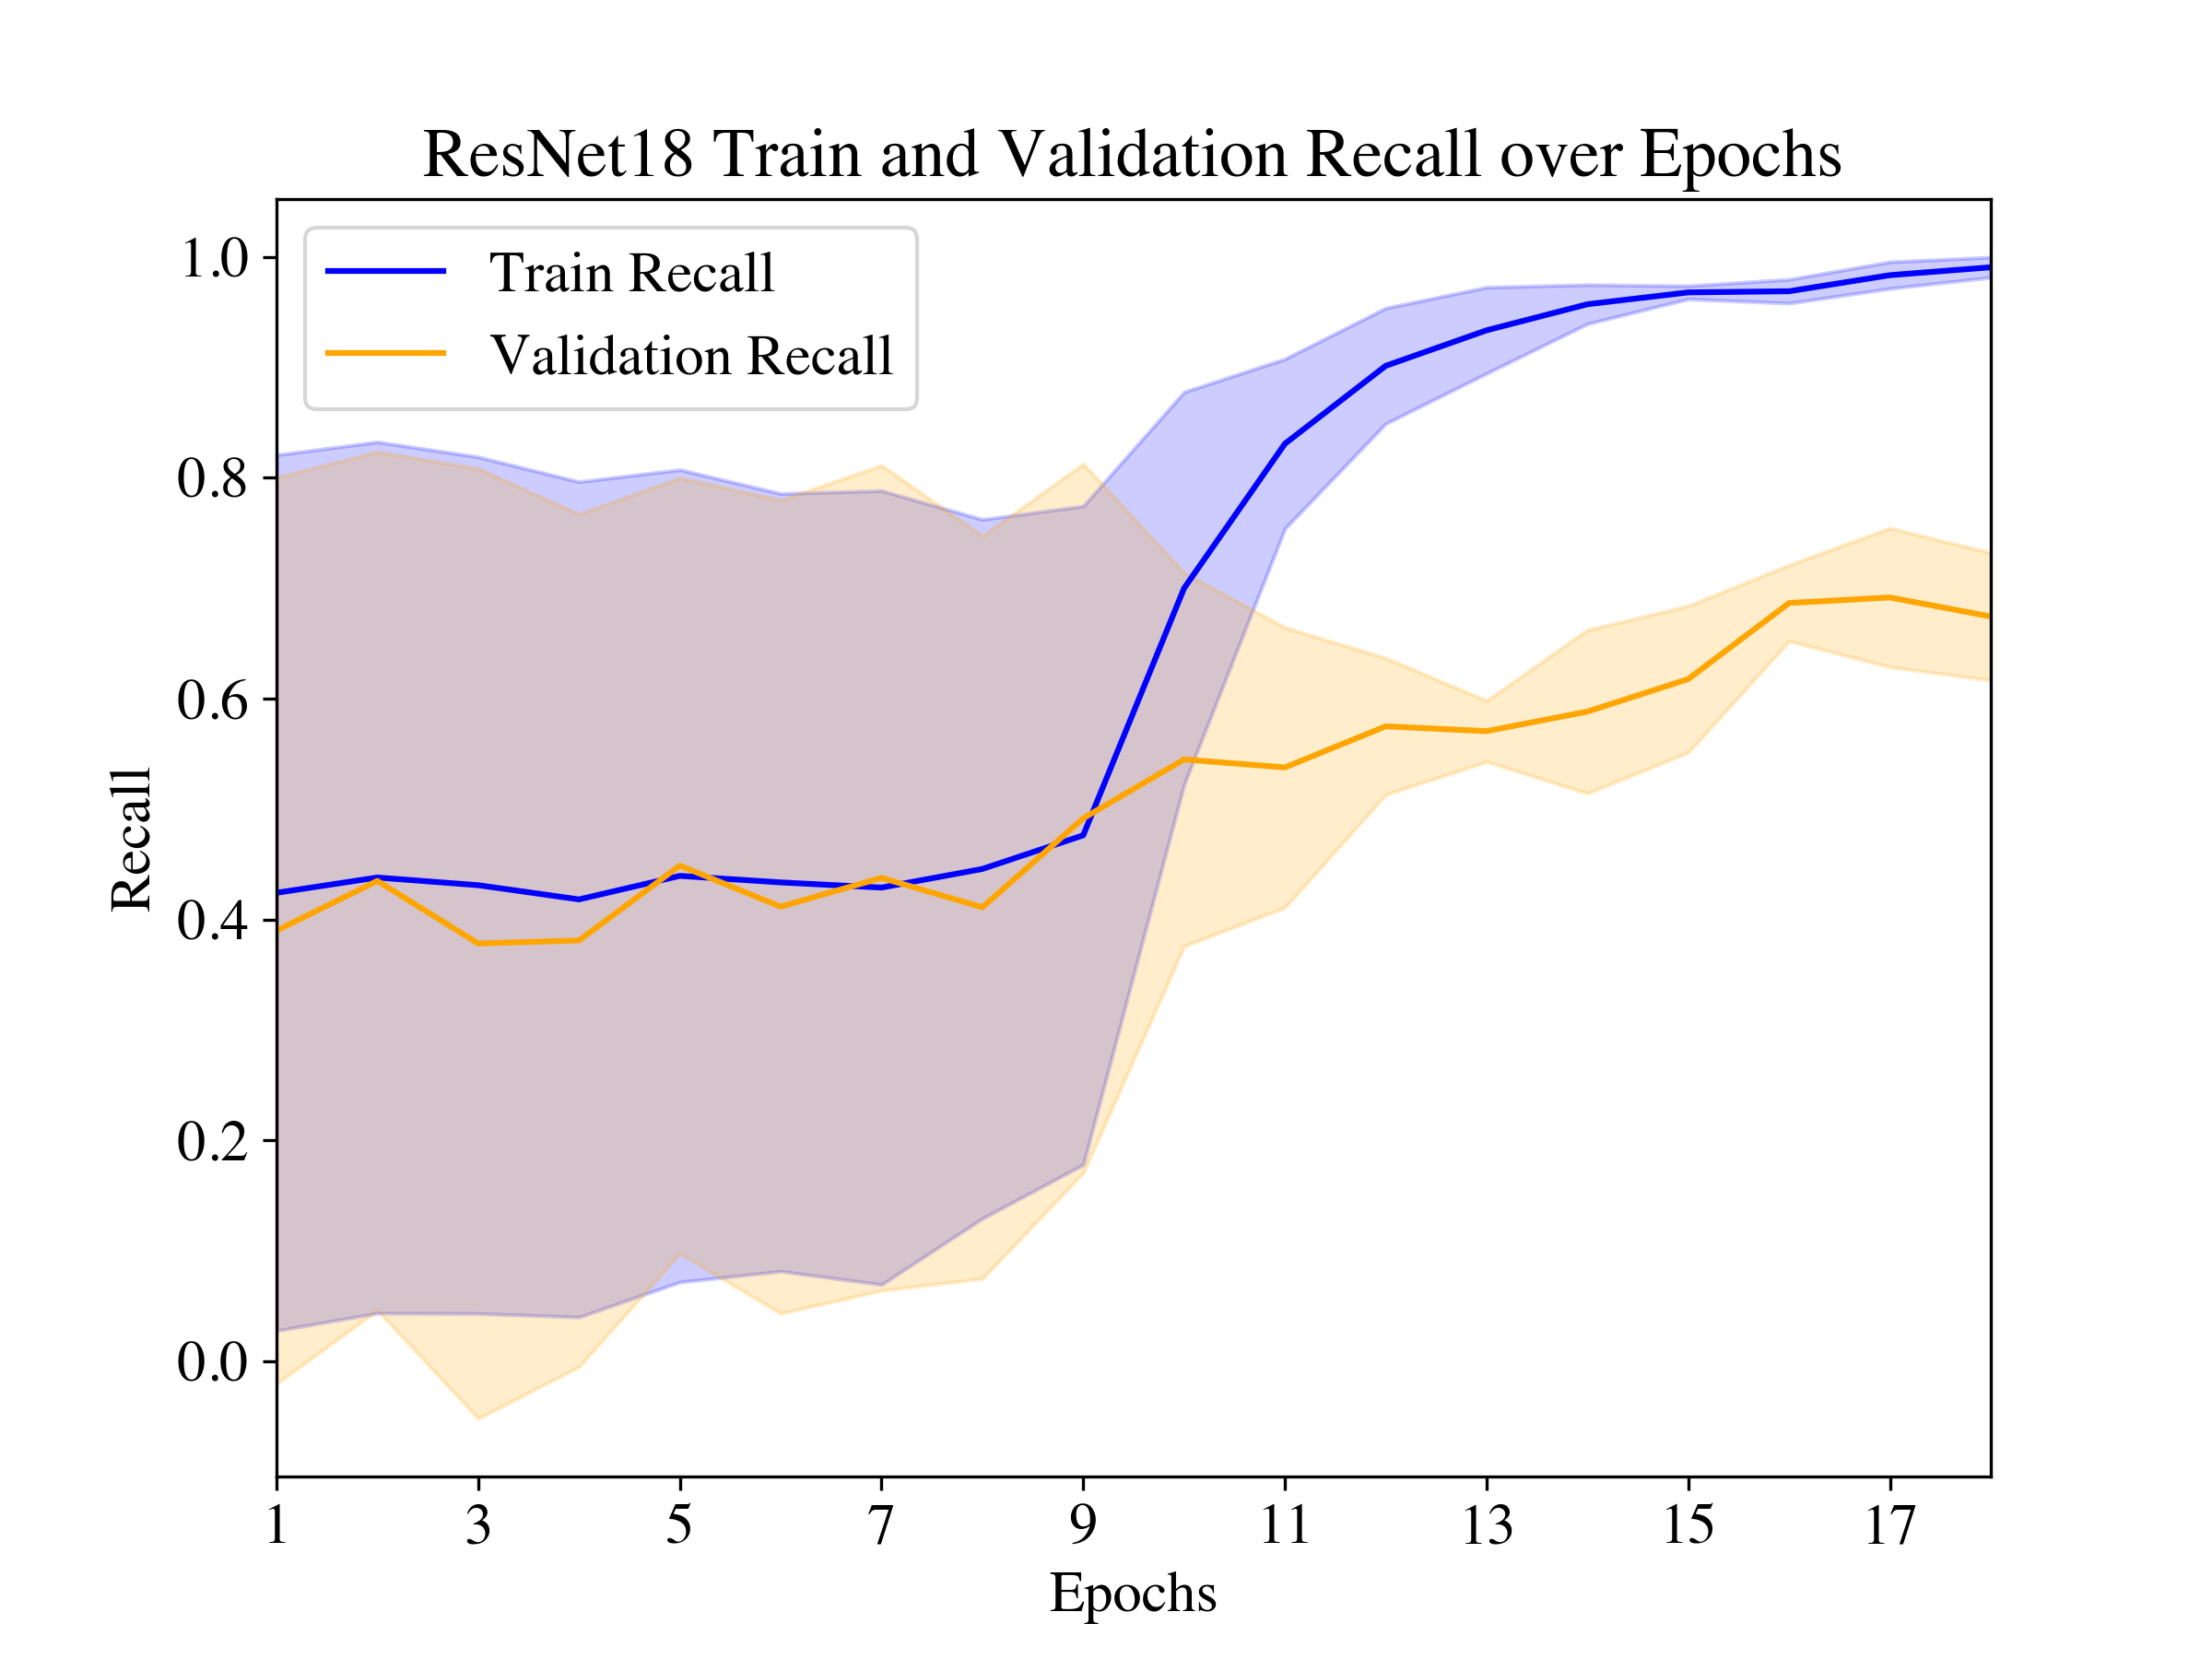
\includegraphics[width=.30\linewidth]{../3d/plots/resnet18/recall_score.png}
\end{center}
\caption{ResNet18 train (blue) and validation (orange) accuracy curve (left) precision curve (center) validation curve (right) with mean and standard deviation. This model was trained on the concatenated Retina Layer d, r, s.}
\end{figure}



\section{Conclusion and Future Work}
Alzheimer's Disease is the most common type of dementia. Traditional methods are often costly and subjective. Classifying Alzheimer's Disease using OCTA images offers a solution that is time and cost effecient. This project demonstrates that deep learning models can be used on OCTA images to successfully classify Alzheimer's Disease with an accuracy of .69. The information from multiple layers also show potential on improving prediction accuracy. The results of this project are comparable with the results using Machine Learning techniques and demonstrate that deep learning models can be used to classify OCTA multilayer images.  Future work includes using a weighted average from the results, or first doing feature extraction on each layer, then concatenating the features. In addition, other deep learning models can be explored such as DenseNet and EffientNET. Lastly, the dataset used in this study is relatively small, future work includes collecting more data to improve the performance of the models.

\section*{Author Contributions Statement}
A.C. conceived the original idea, developed the methodology, performed the experiments, analyzed the results and wrote the manuscript.


\bibliography{iclr2021_conference}
\bibliographystyle{iclr2021_conference}

\appendix
\section{Appendix}
All code can be found at \url{https://github.com/yuehtingchen/cv-final-project}.
Additional training results can be found below.

\begin{figure}[h]
   \begin{center}
   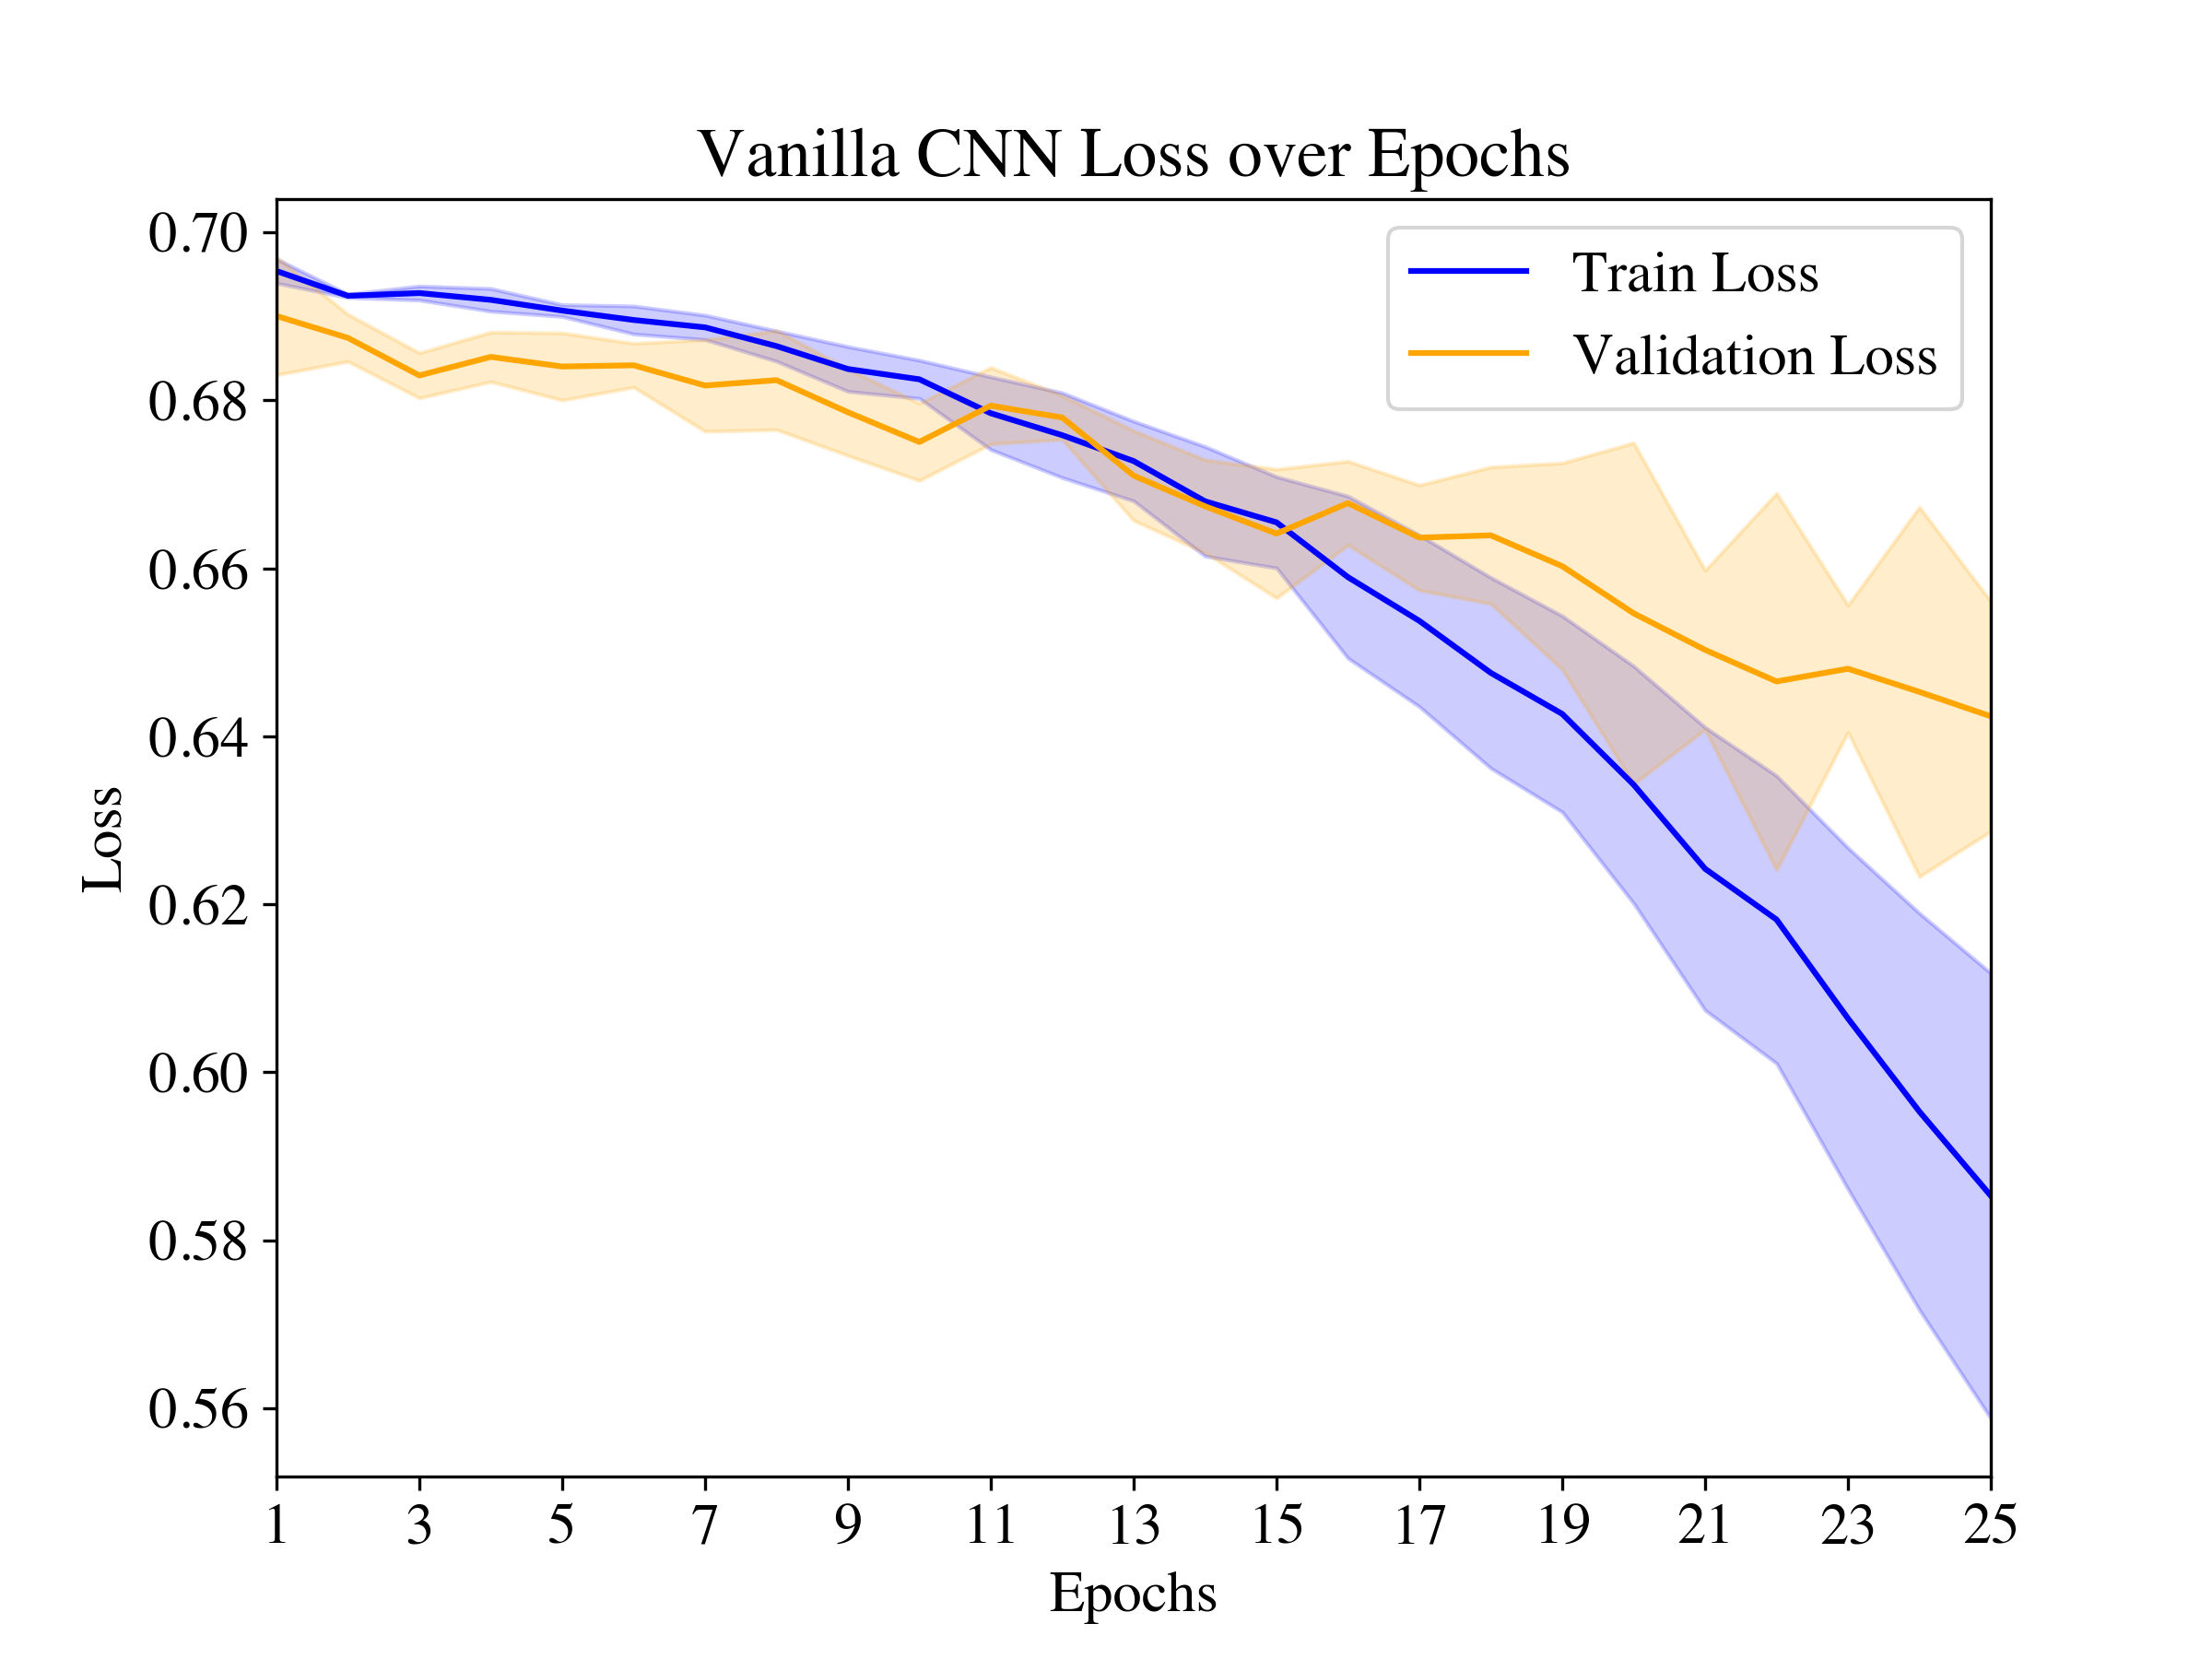
\includegraphics[width=.4\linewidth]{../plots/cnn/loss.png}
   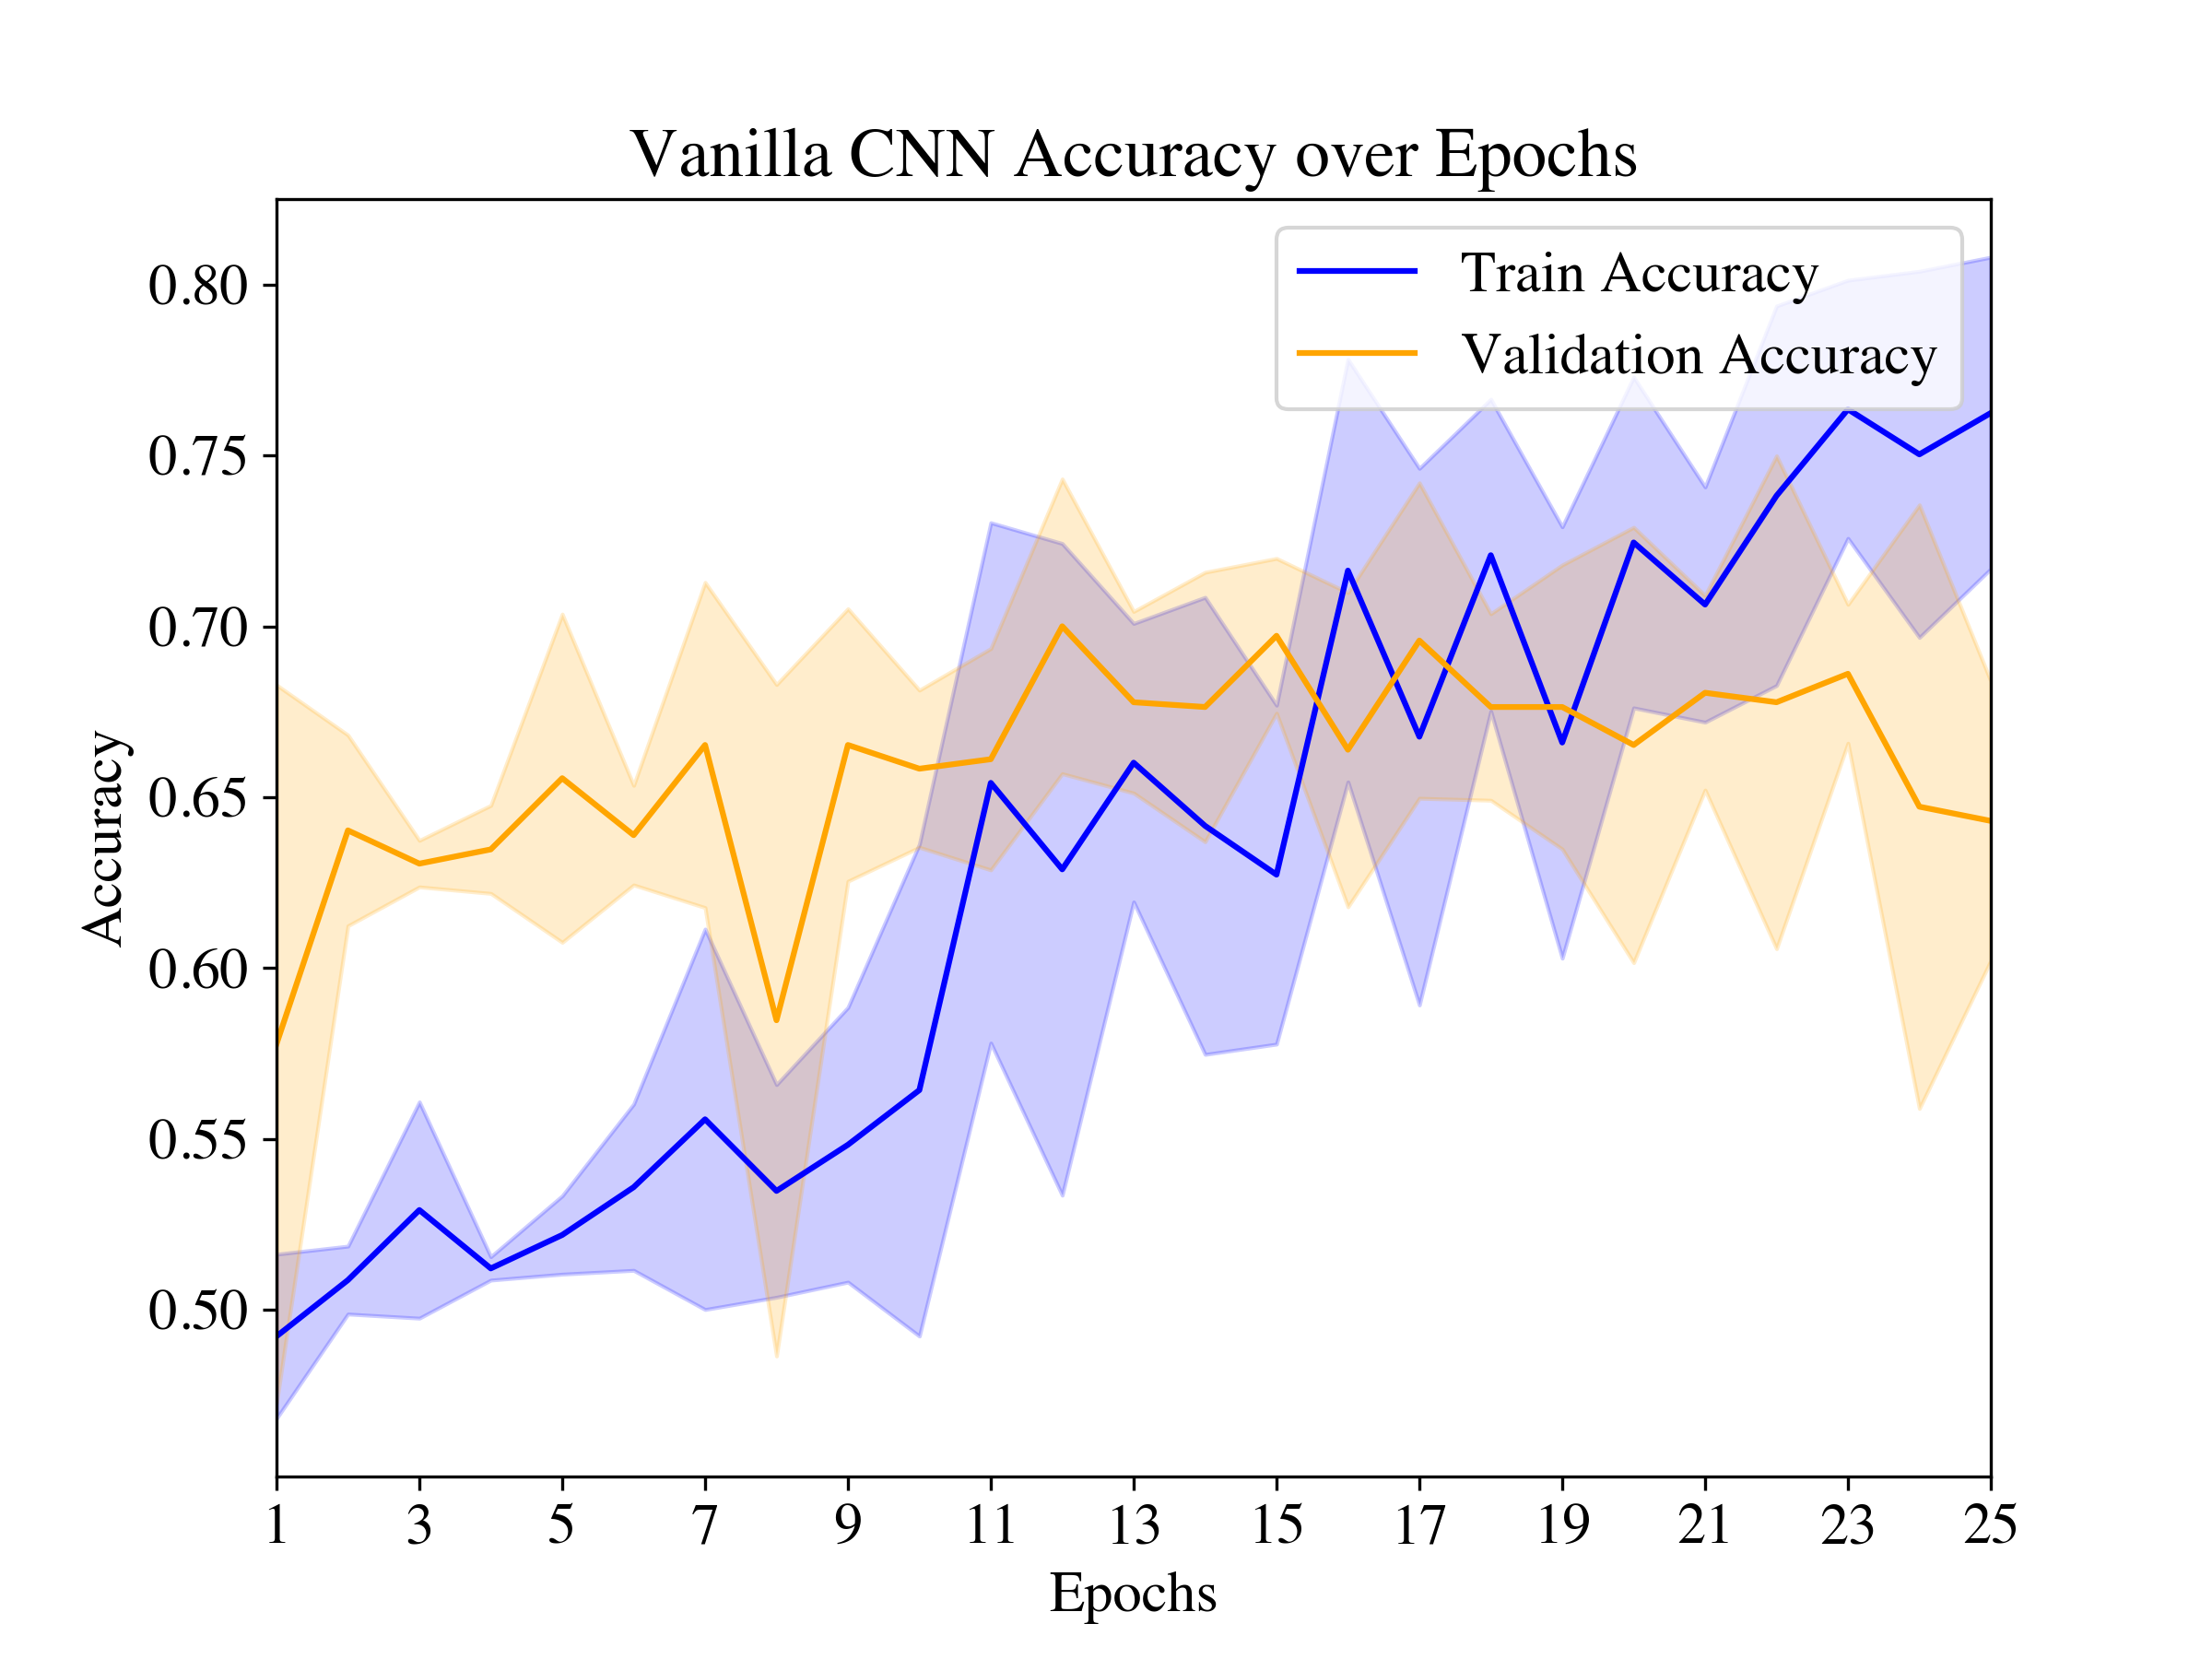
\includegraphics[width=.4\linewidth]{../plots/cnn/accuracy.png}
   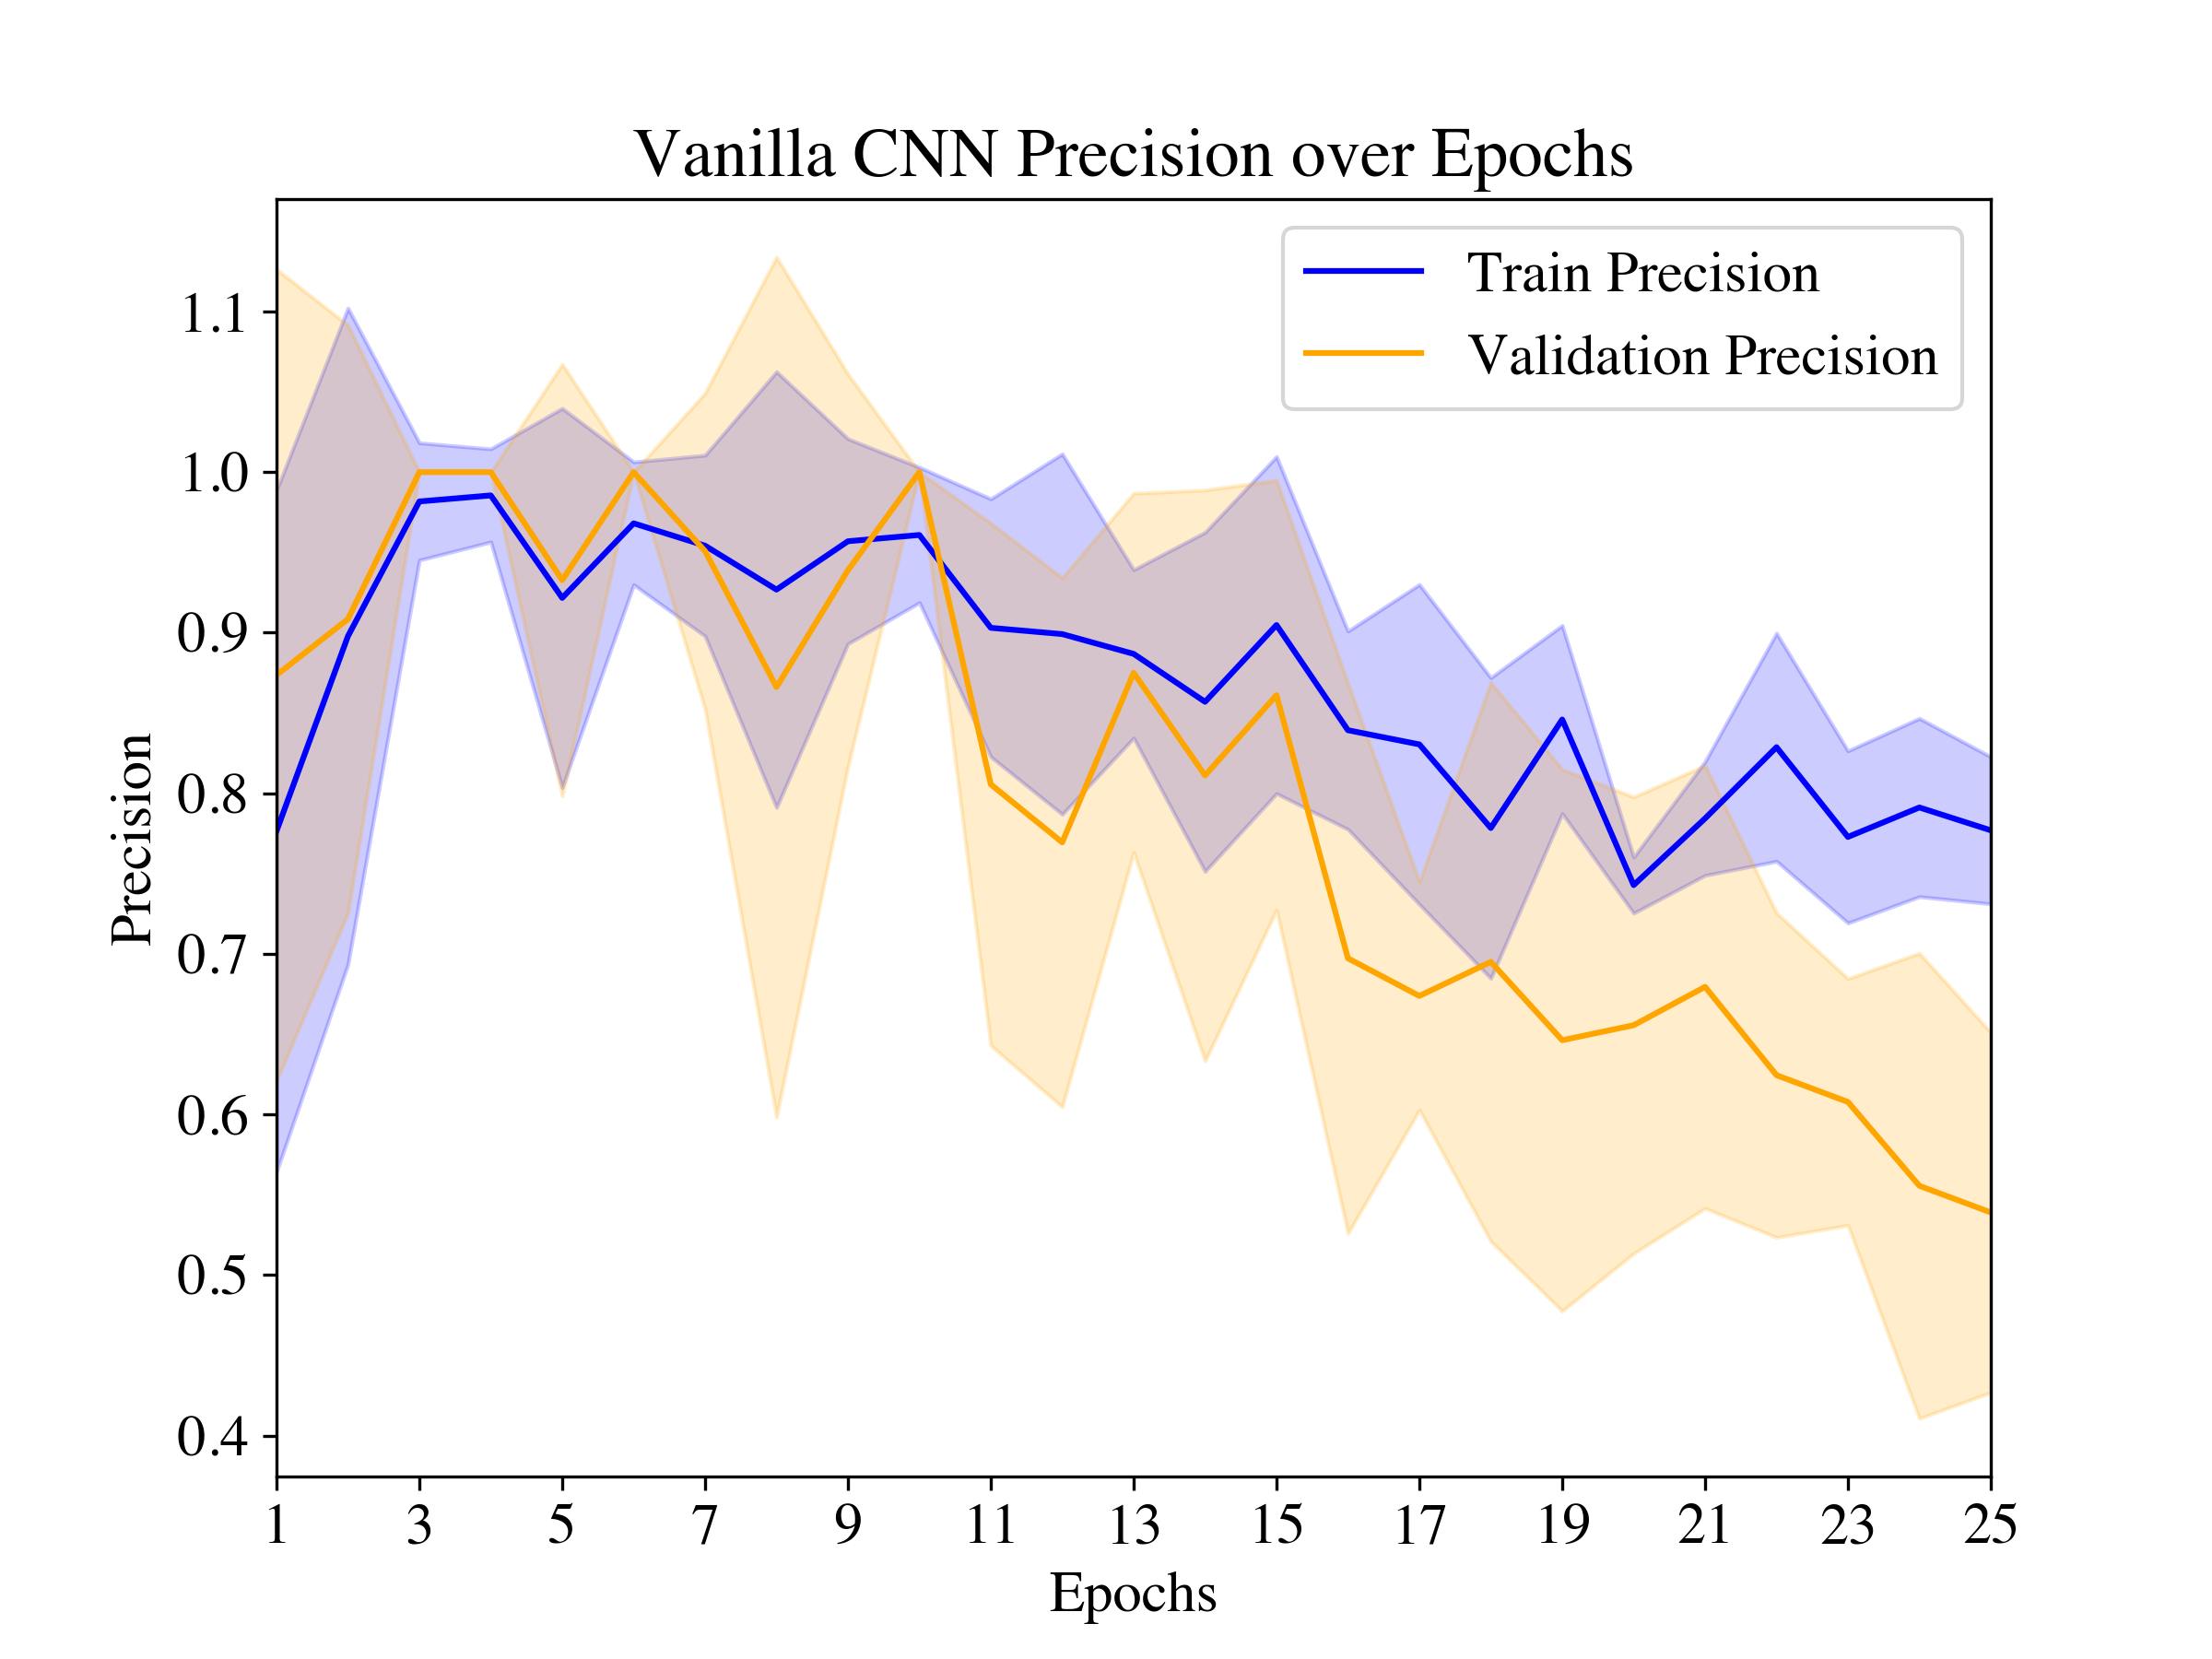
\includegraphics[width=.4\linewidth]{../plots/cnn/precision.png}
   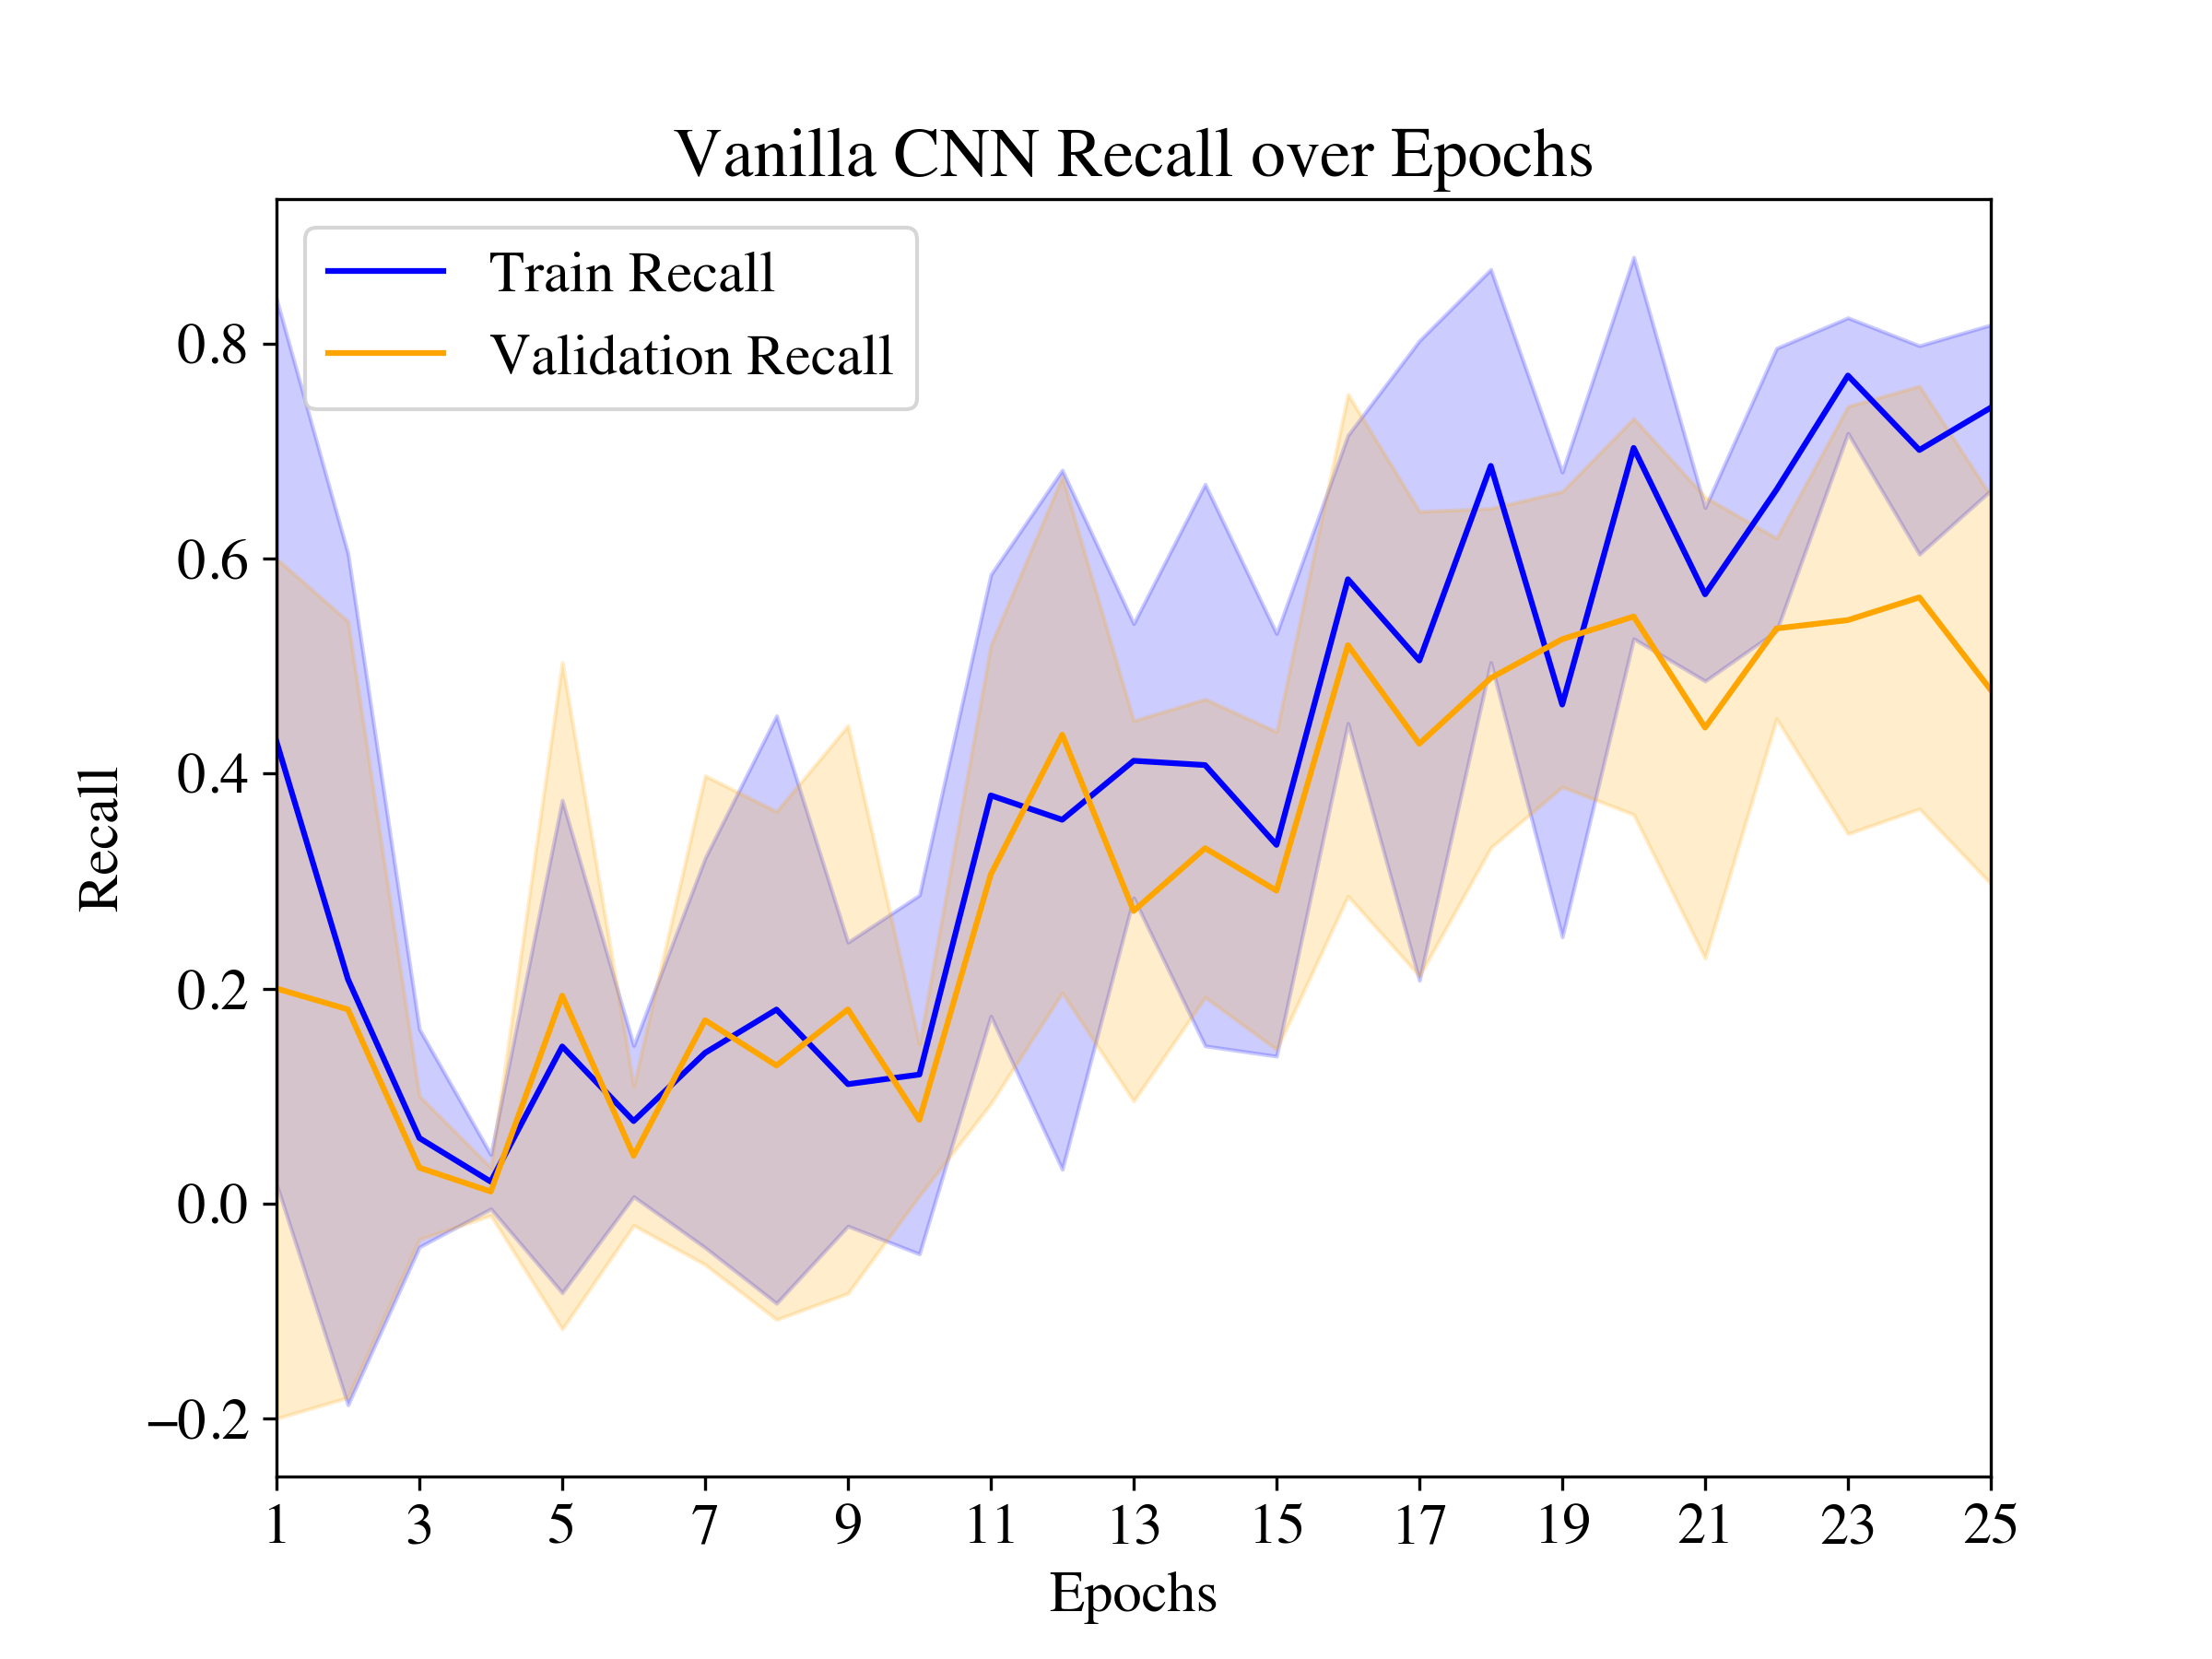
\includegraphics[width=.4\linewidth]{../plots/cnn/recall.png}
   \end{center}
   \caption{VanillaCNN train (blue) and validation (orange) loss curve (top left), accuracy curve (top right) precision curve (bottom left) validation curve (bottom right) with mean and standard deviation. This model was trained on the Retina Layer R.}
\end{figure}

\begin{figure}[h]
   \begin{center}
   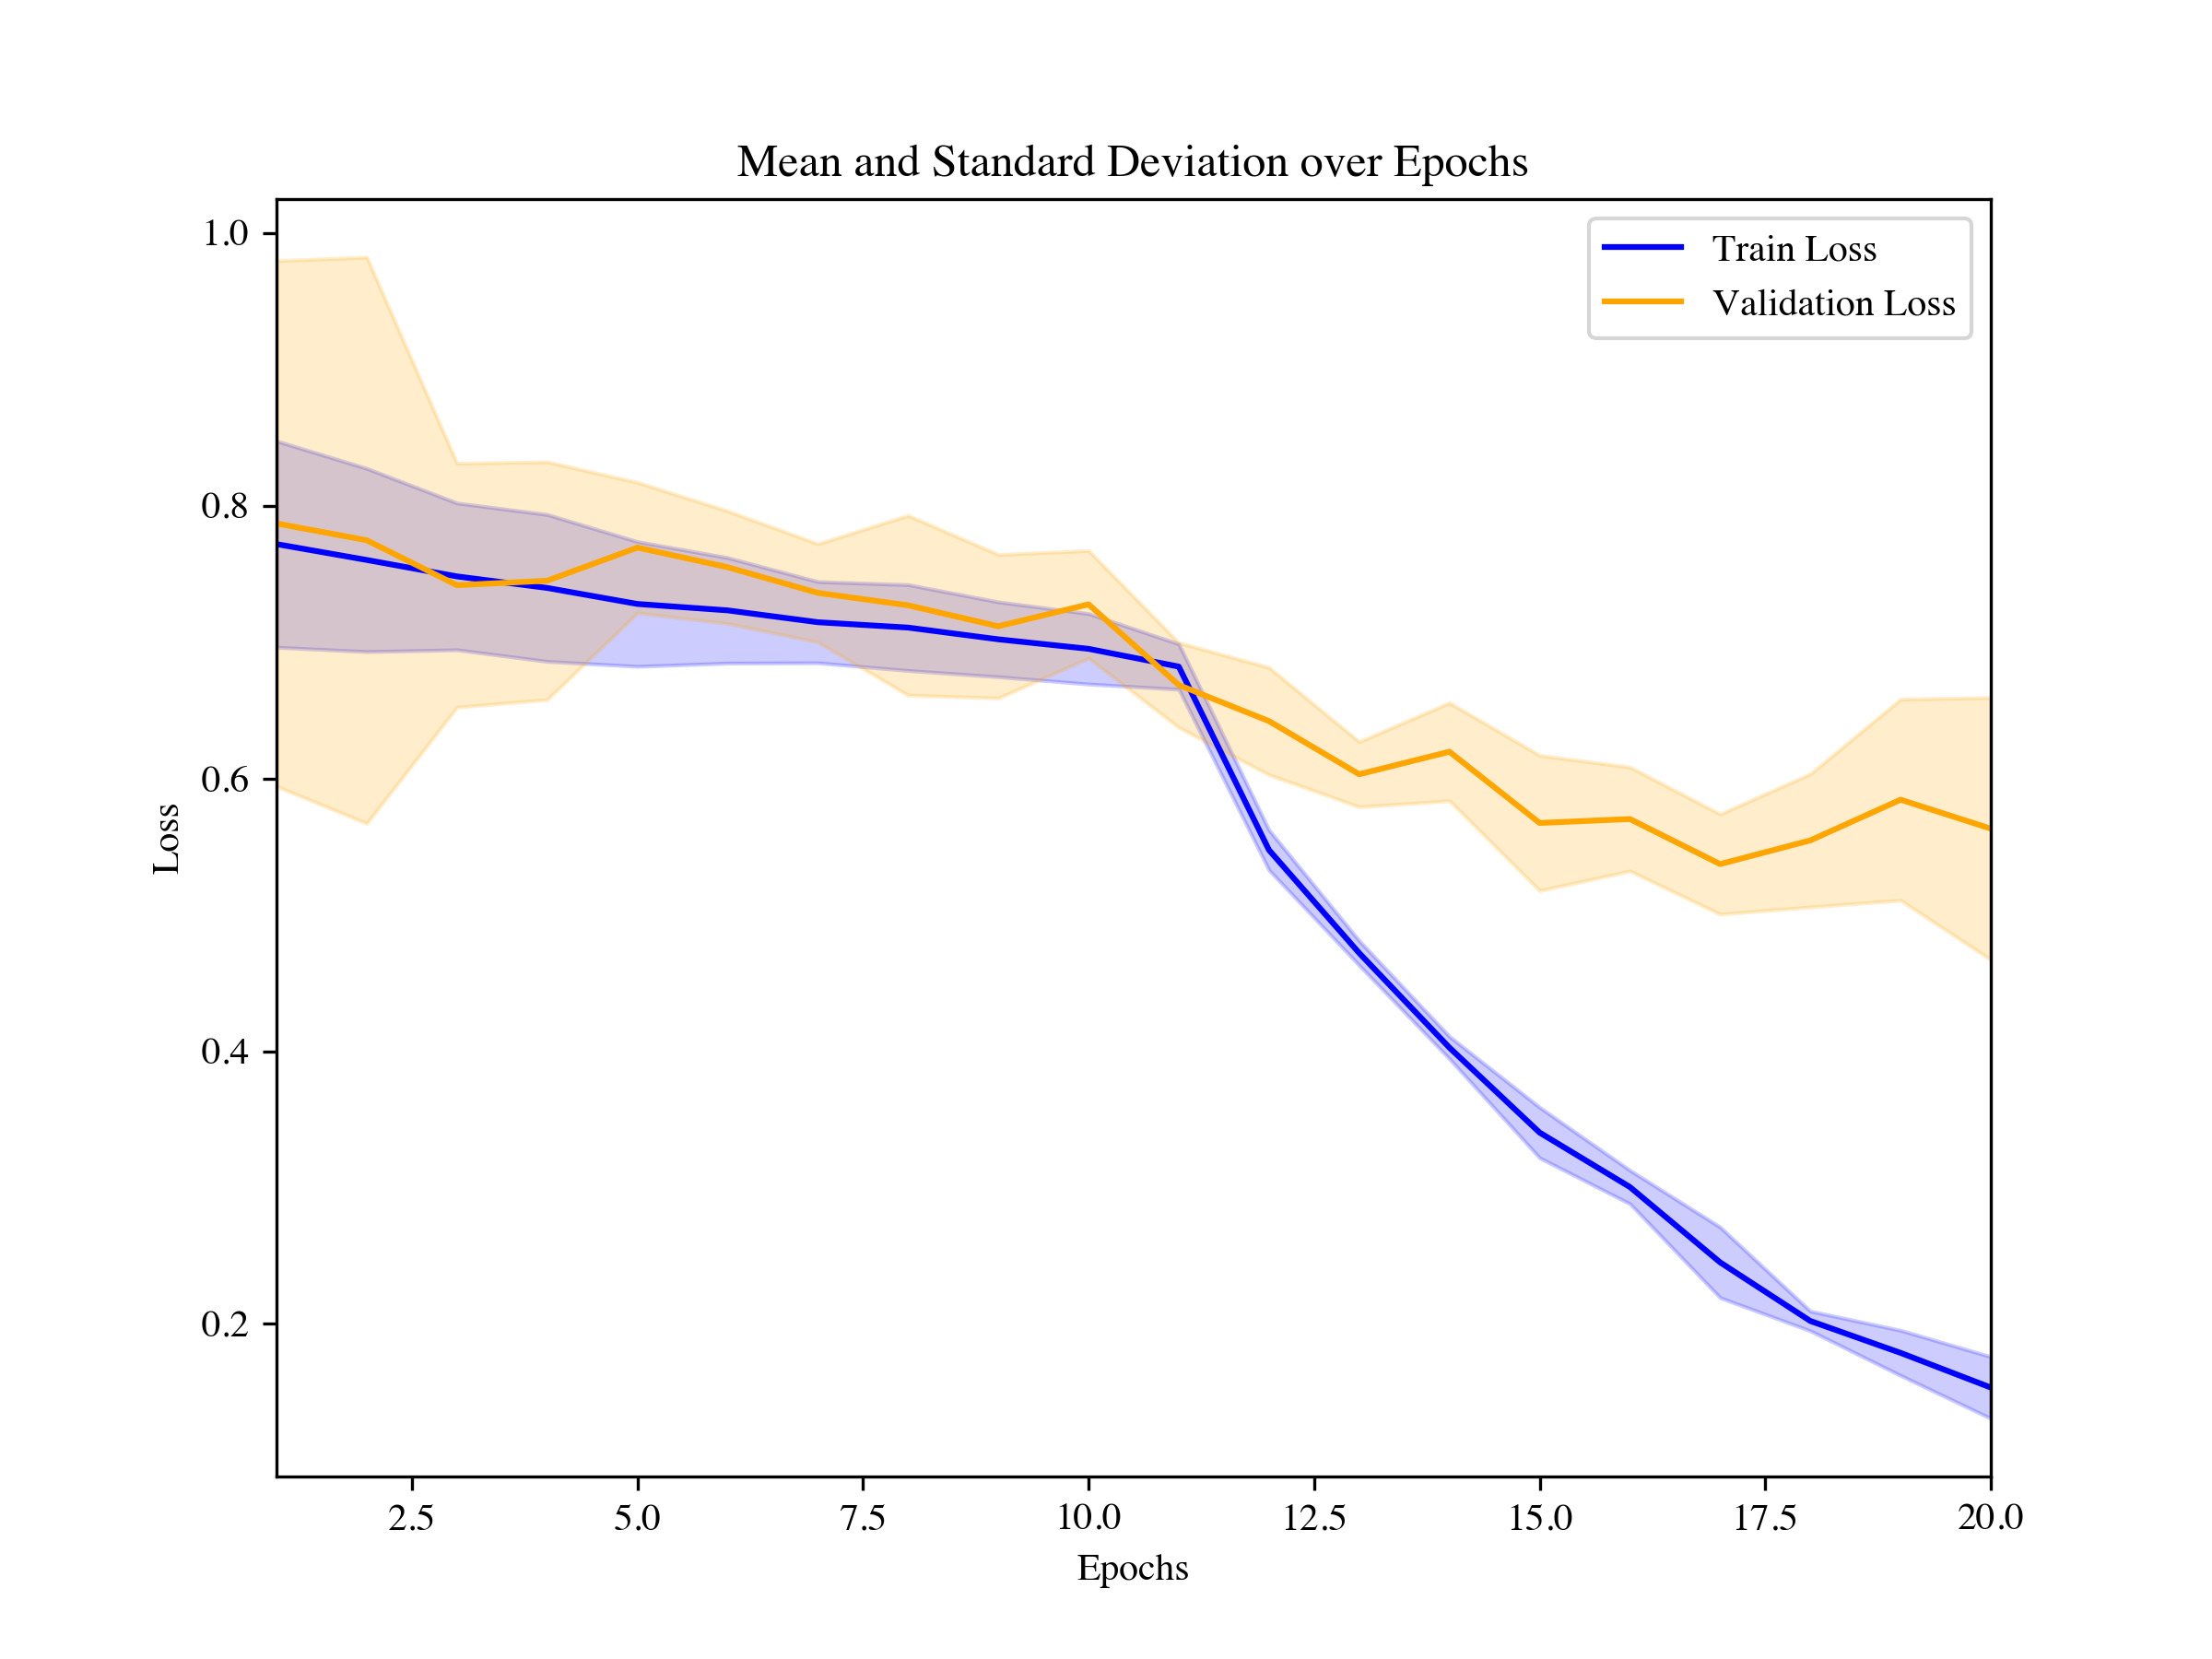
\includegraphics[width=.4\linewidth]{../plots/resnet18/loss.png}
   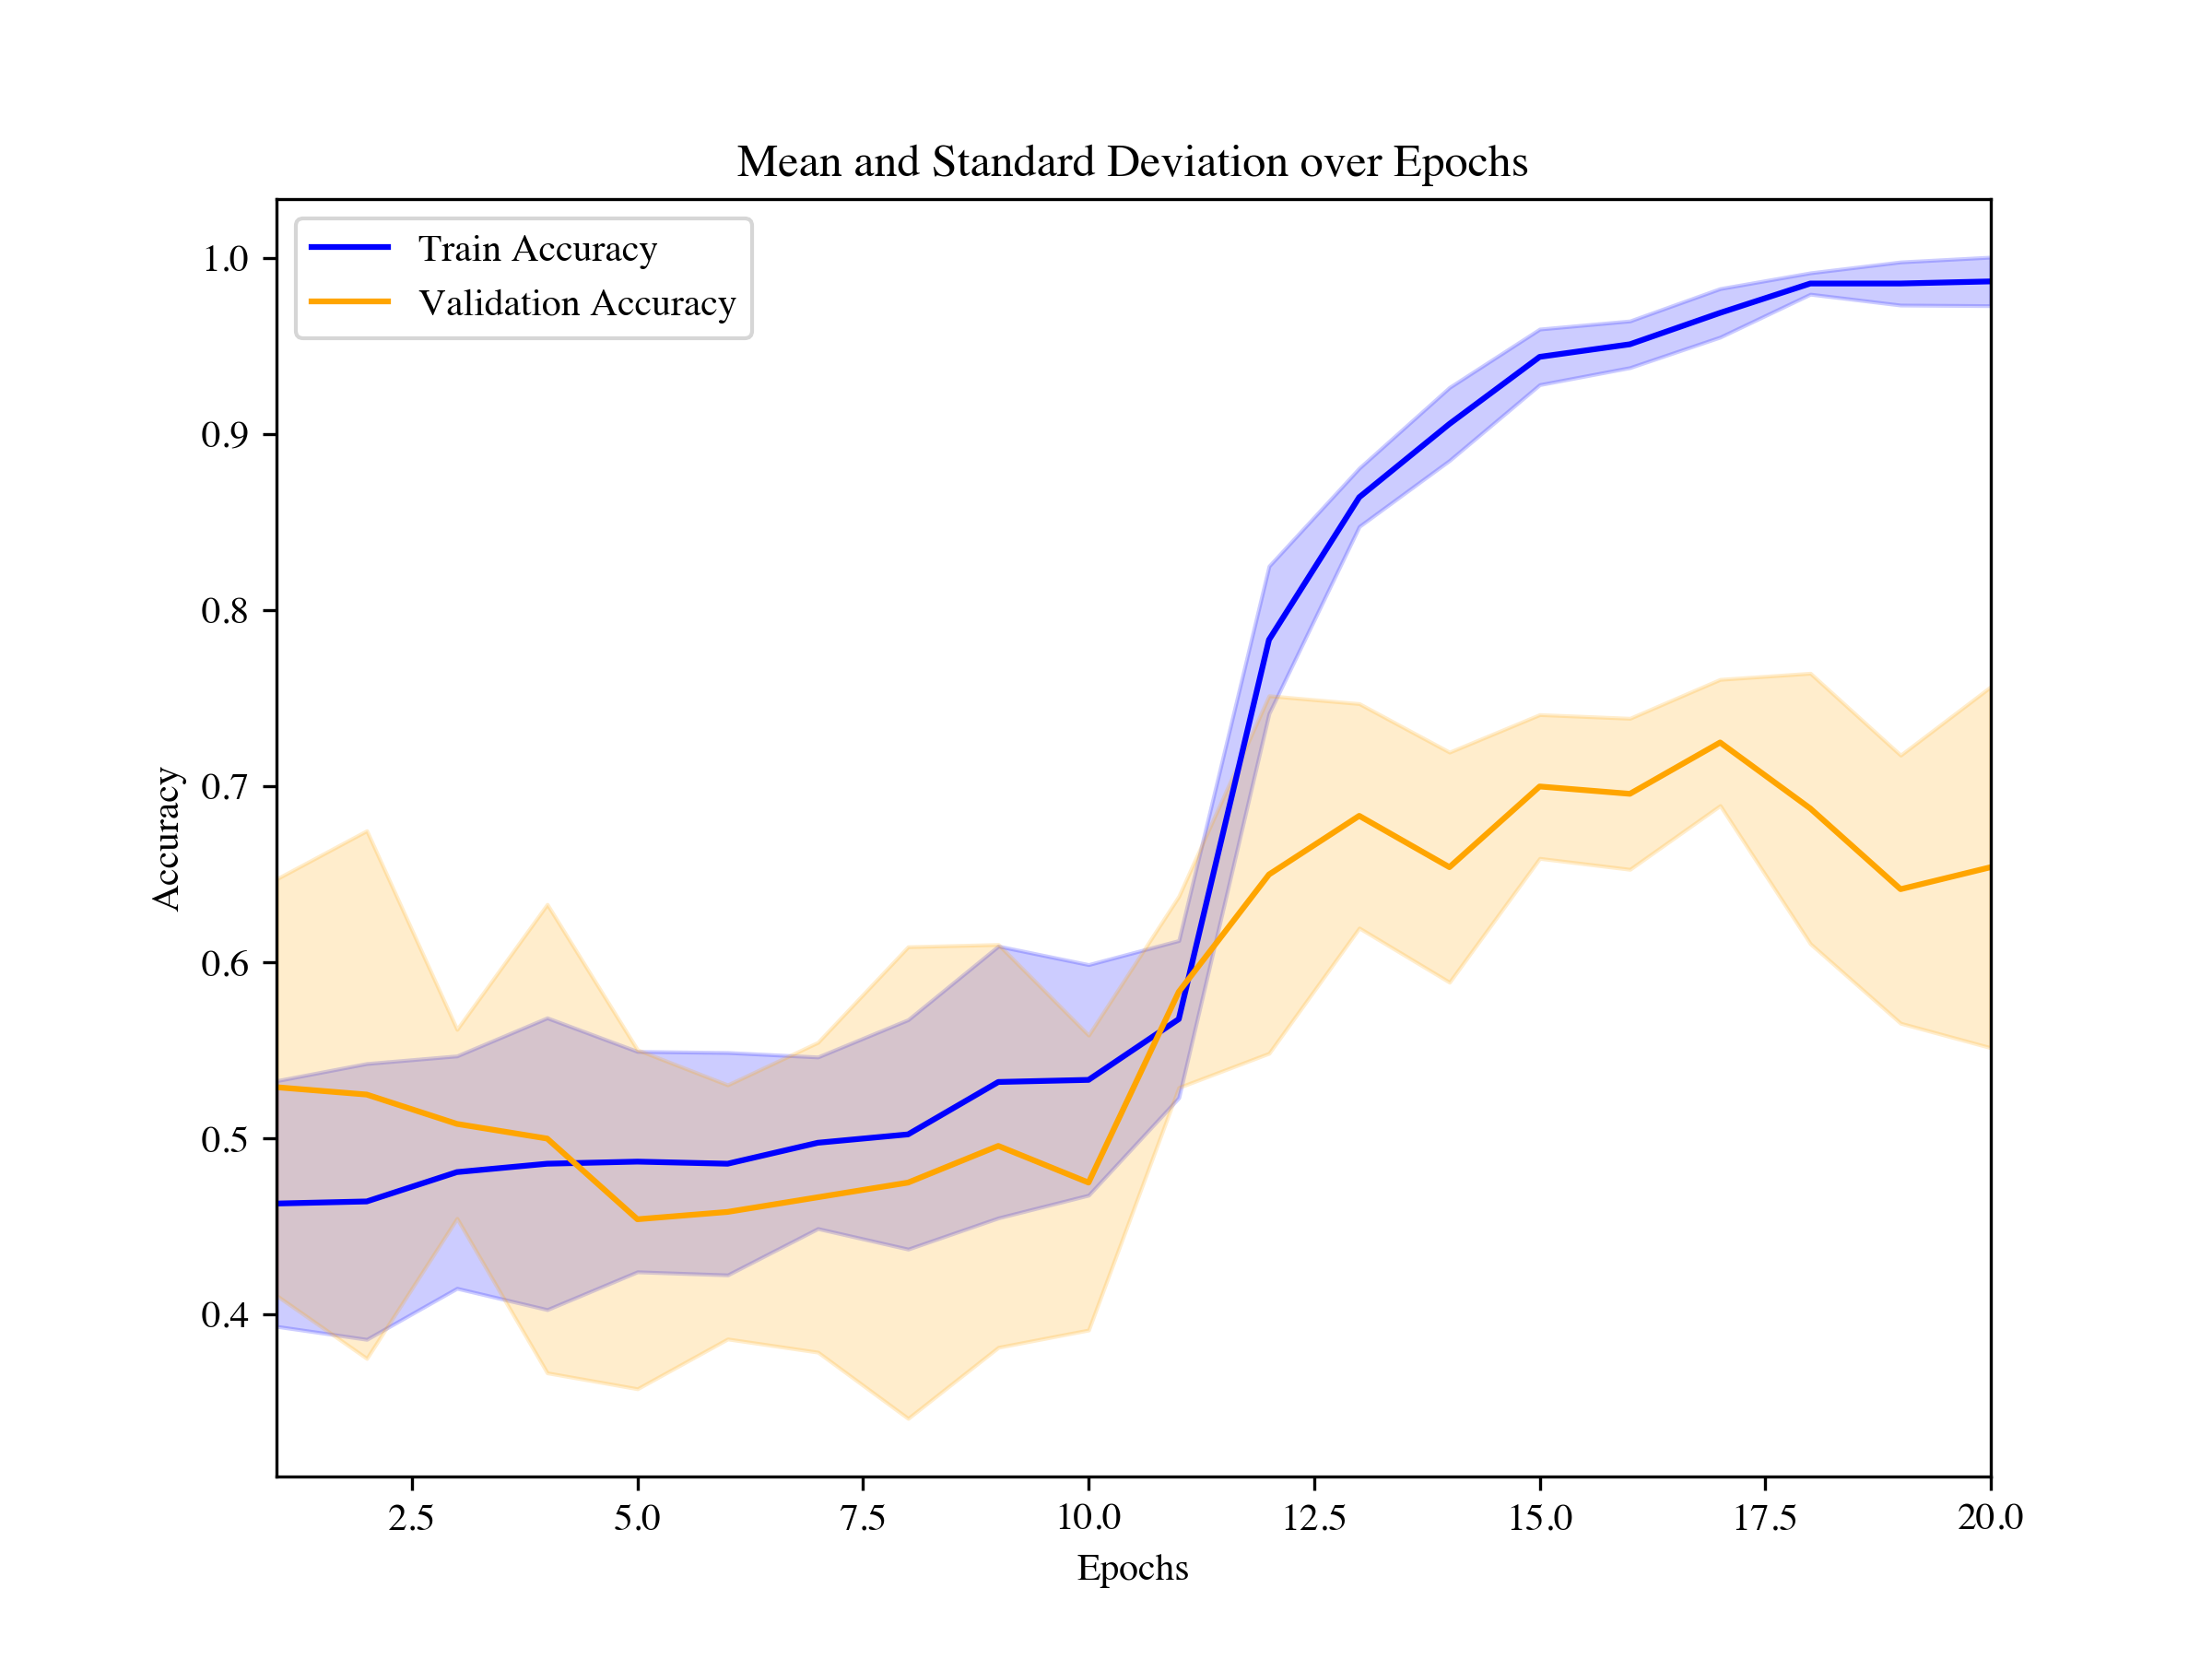
\includegraphics[width=.4\linewidth]{../plots/resnet18/accuracy.png}
   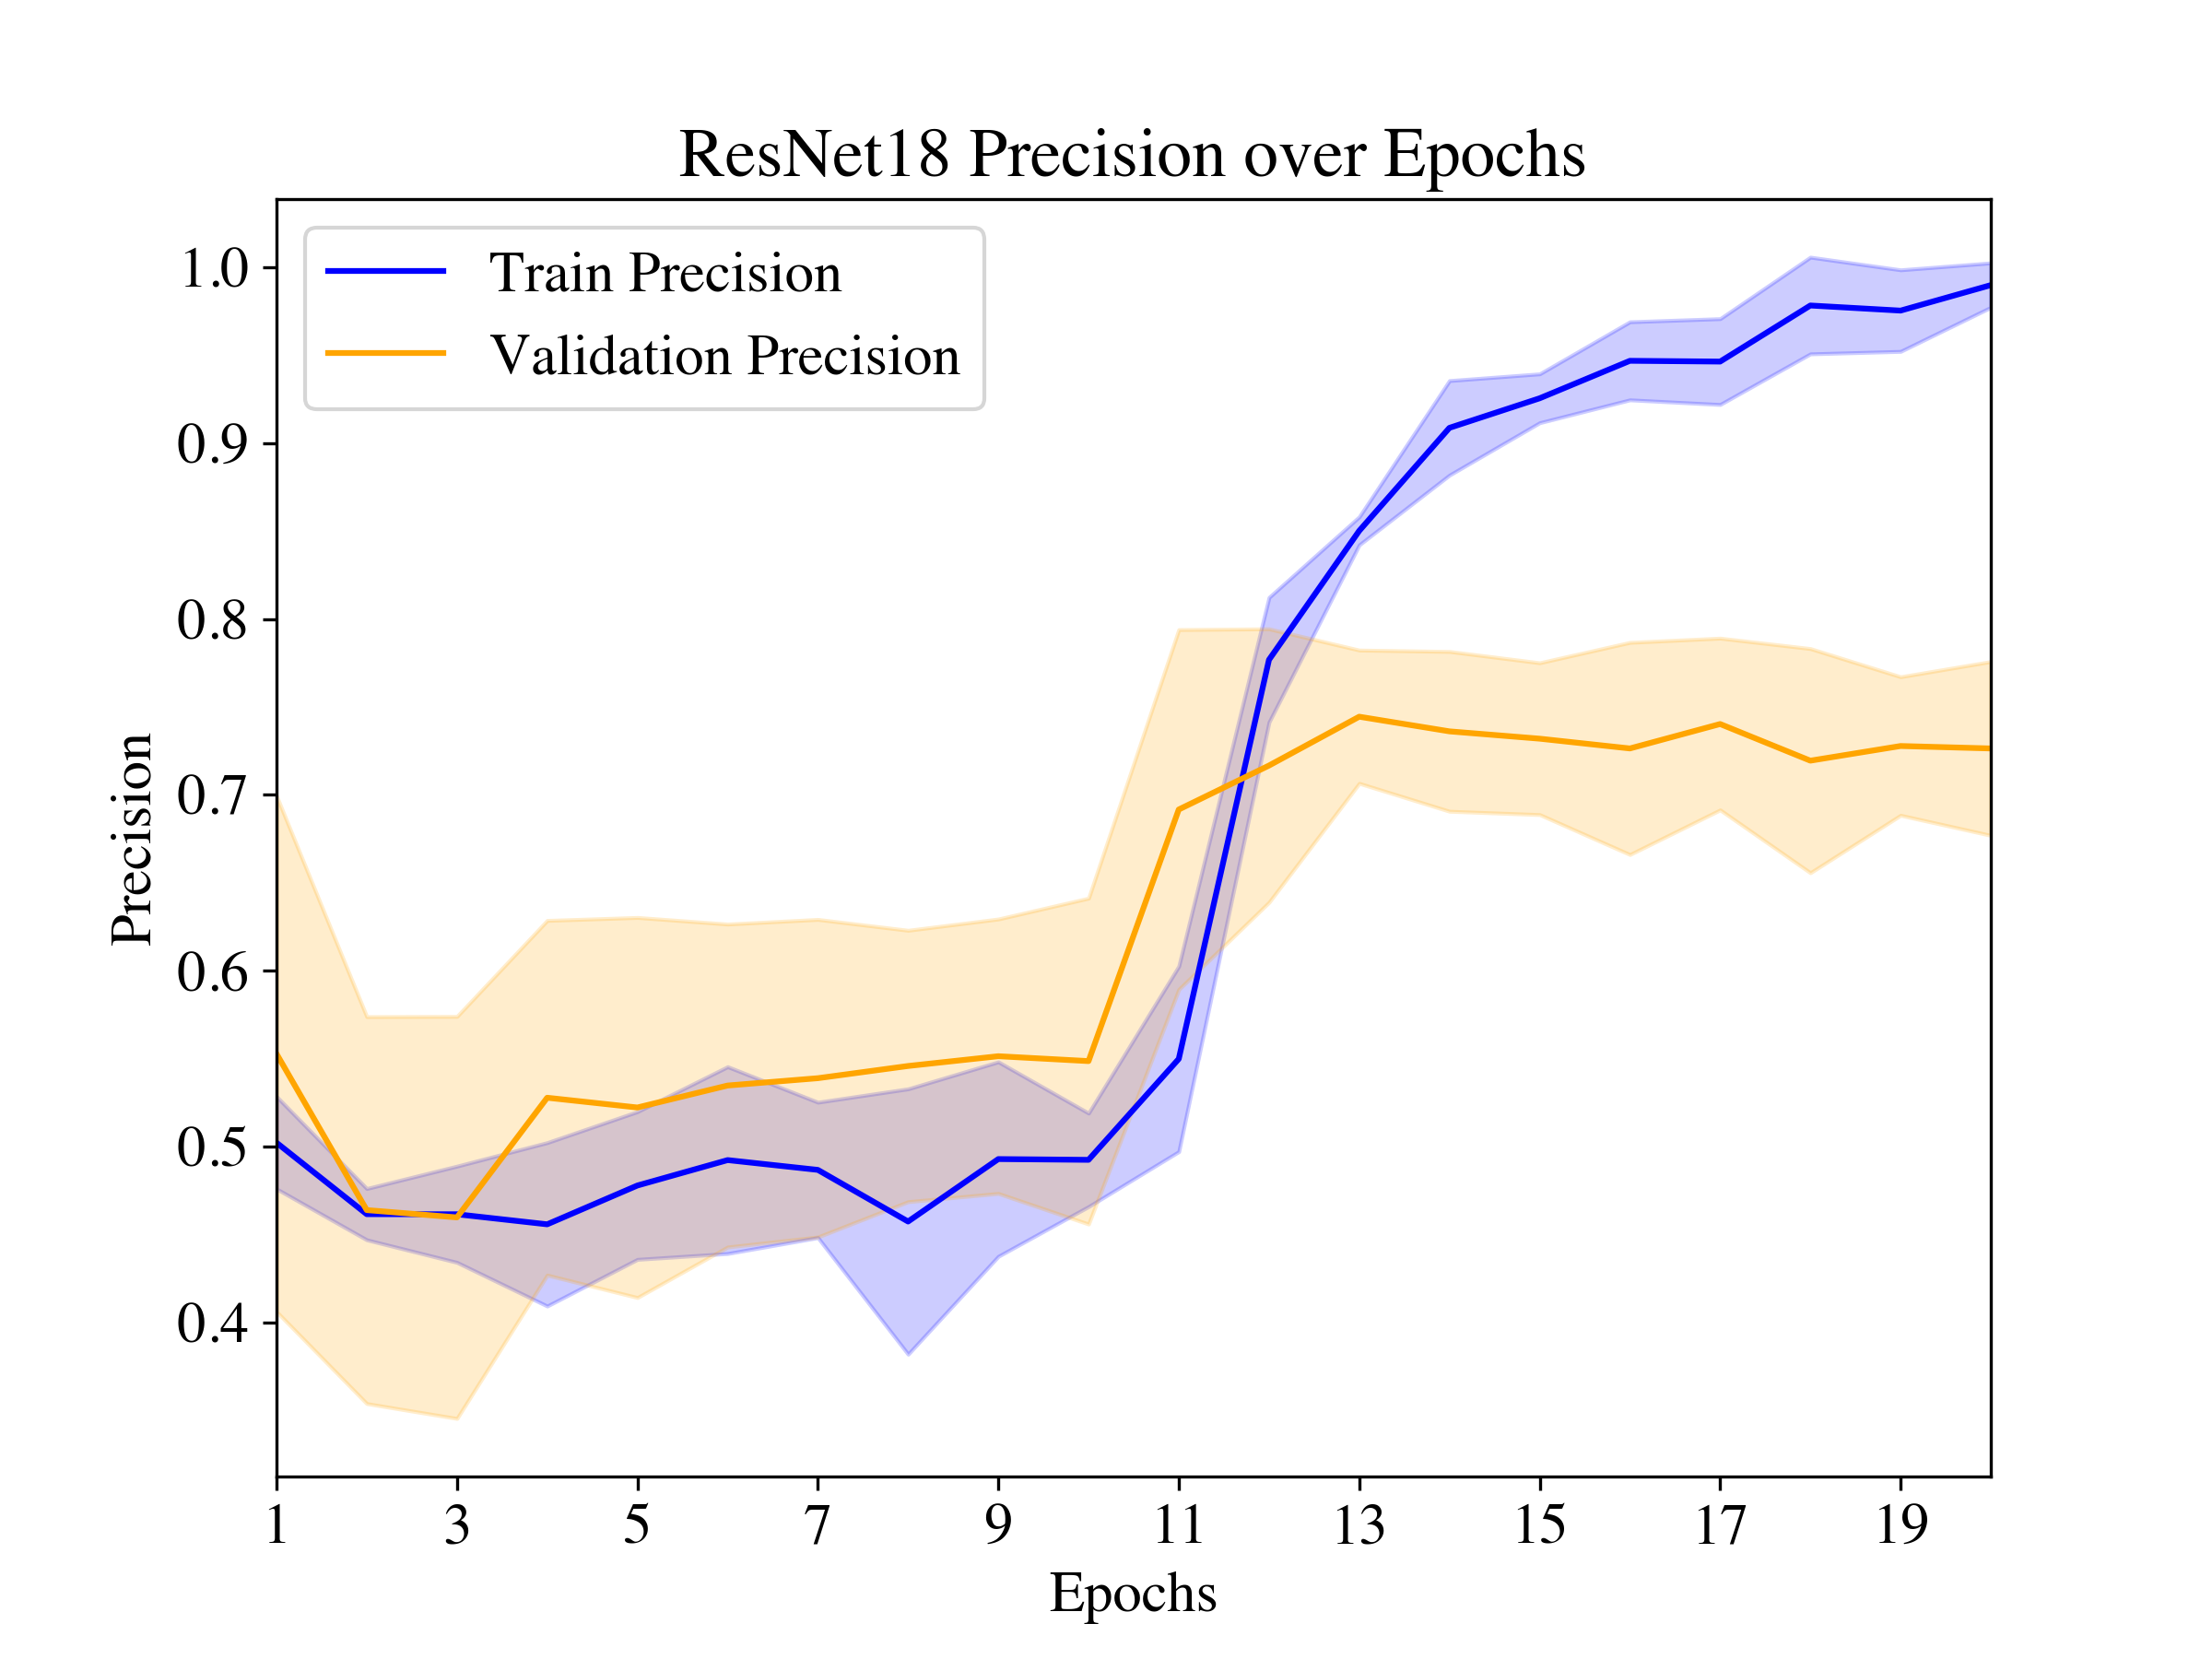
\includegraphics[width=.4\linewidth]{../plots/resnet18/precision.png}
   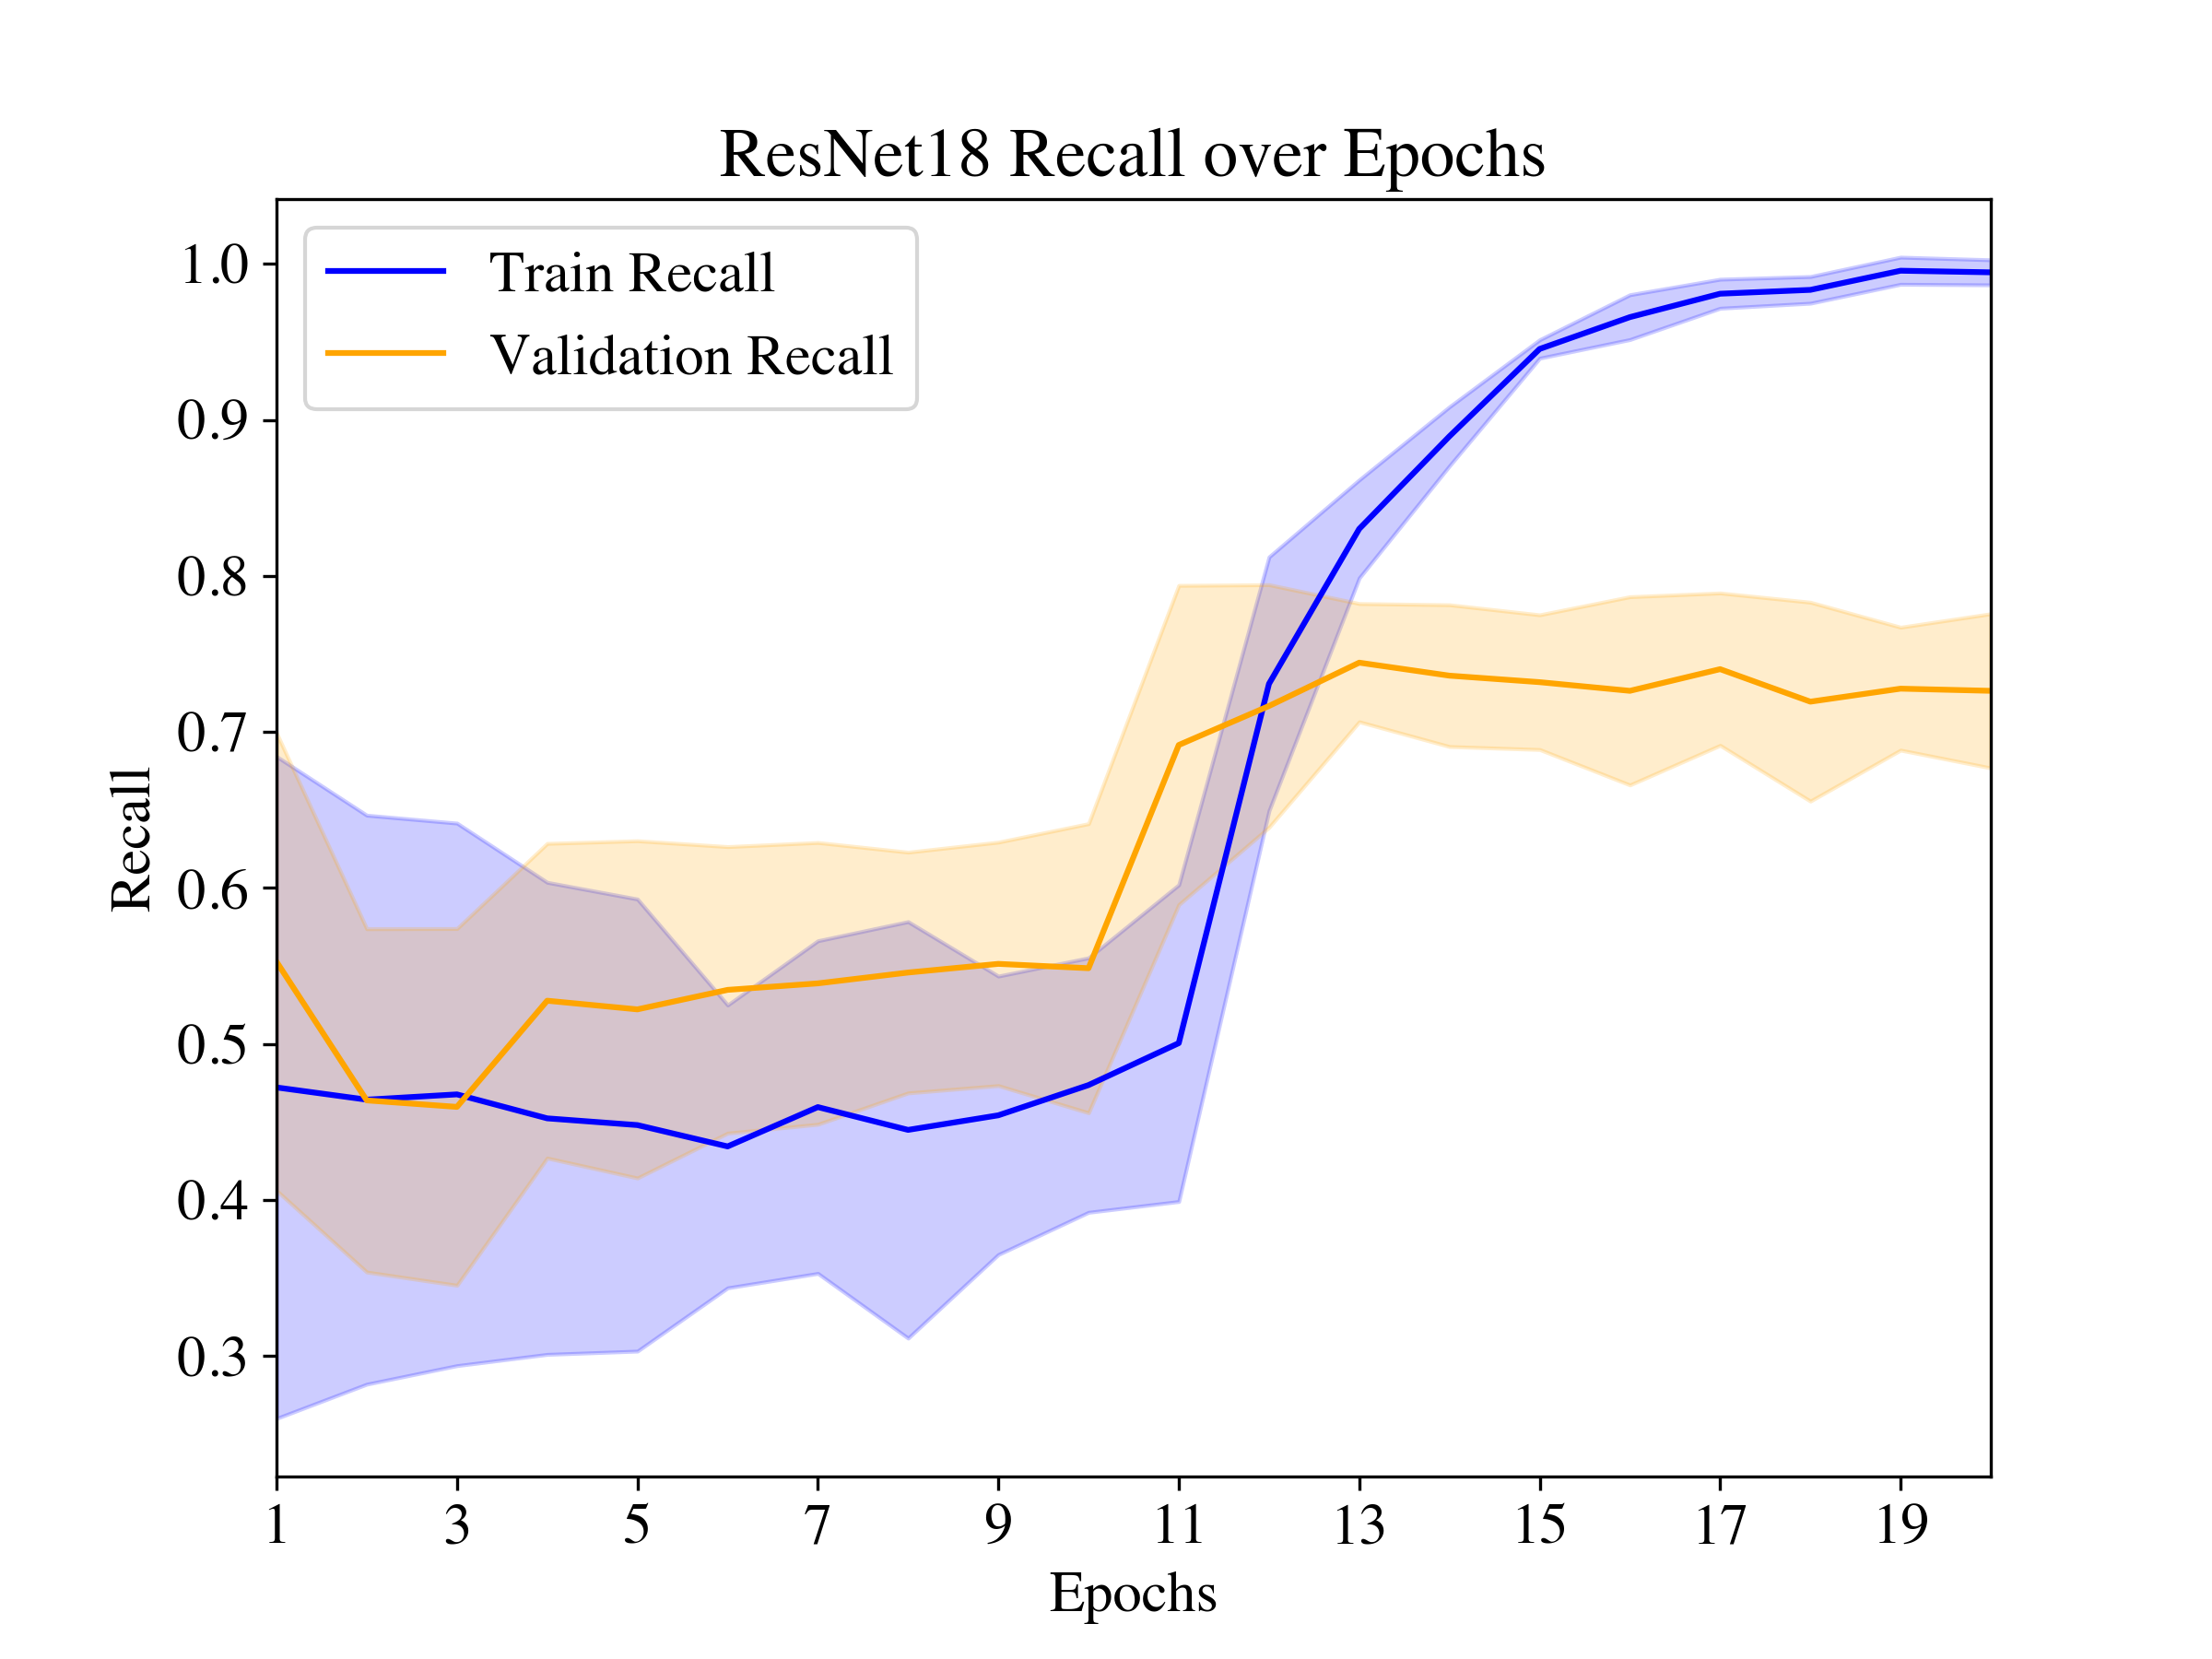
\includegraphics[width=.4\linewidth]{../plots/resnet18/recall.png}
   \end{center}
   \caption{ResNet18 train (blue) and validation (orange) loss curve (top left), accuracy curve (top right) precision curve (bottom left) validation curve (bottom right) with mean and standard deviation. This model was trained on the Retina Layer R.}
\end{figure}

\begin{figure}[h]
\begin{center}
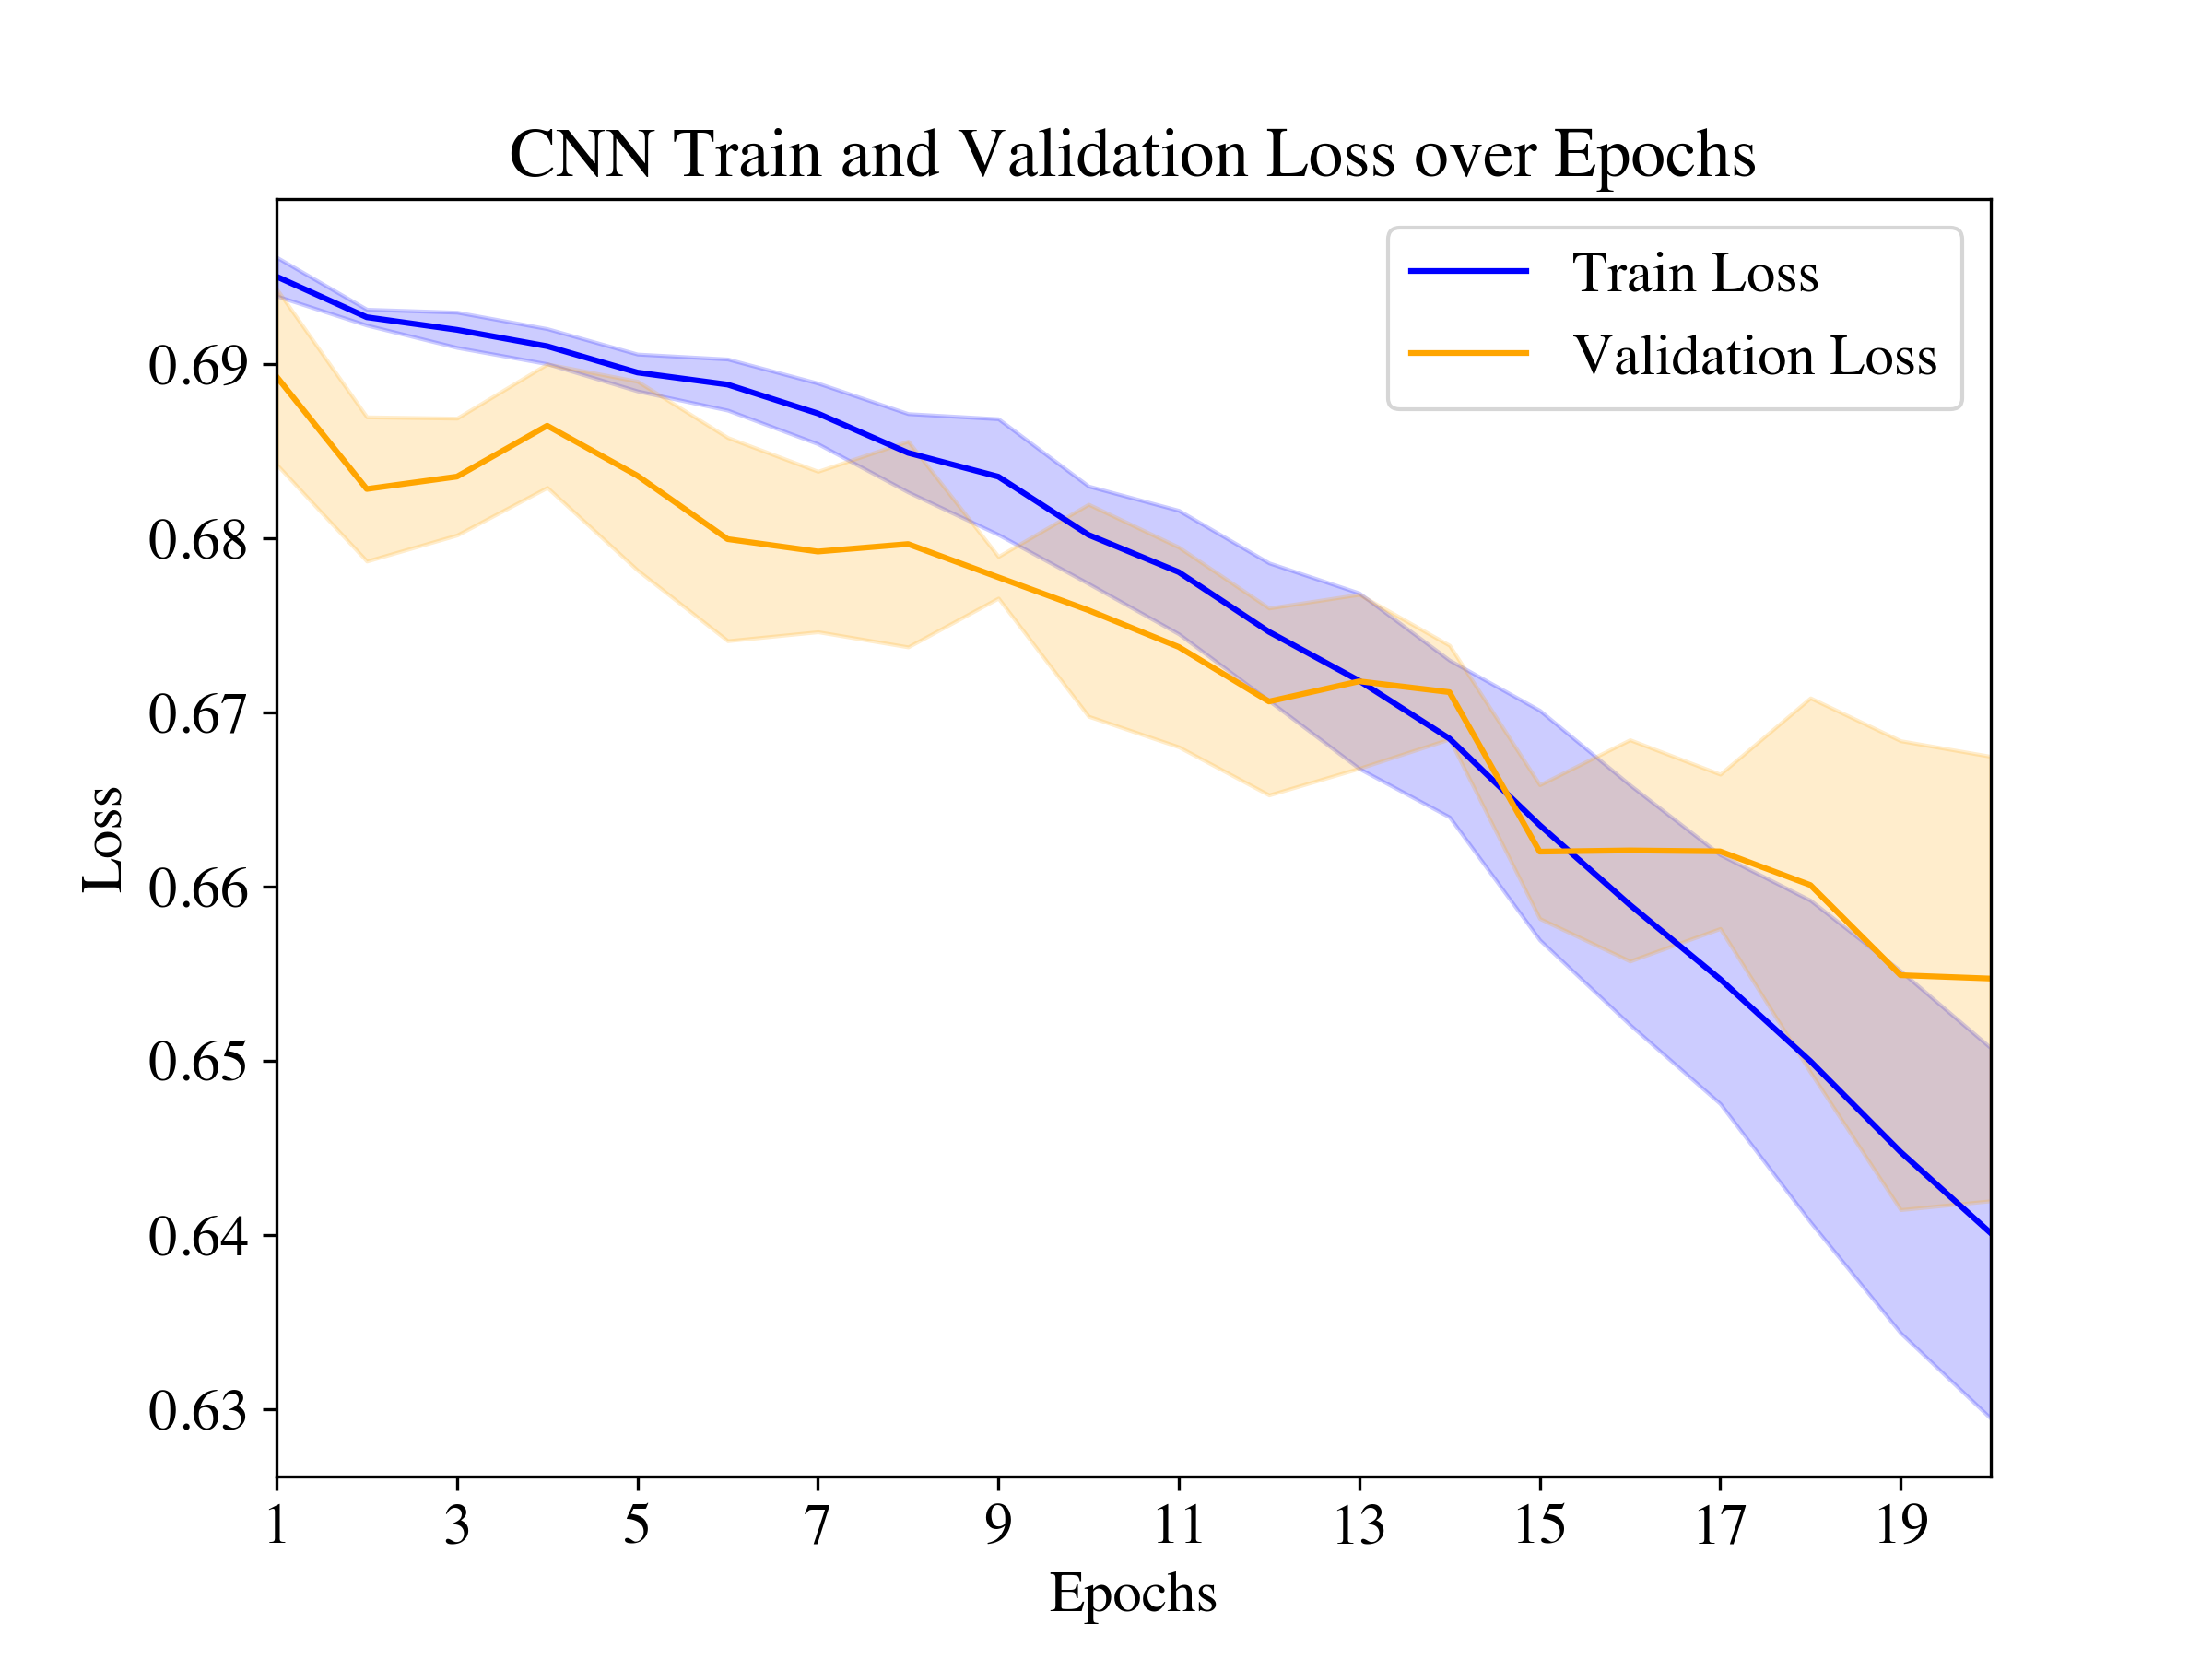
\includegraphics[width=.4\linewidth]{../3d/plots/cnn/loss.png}
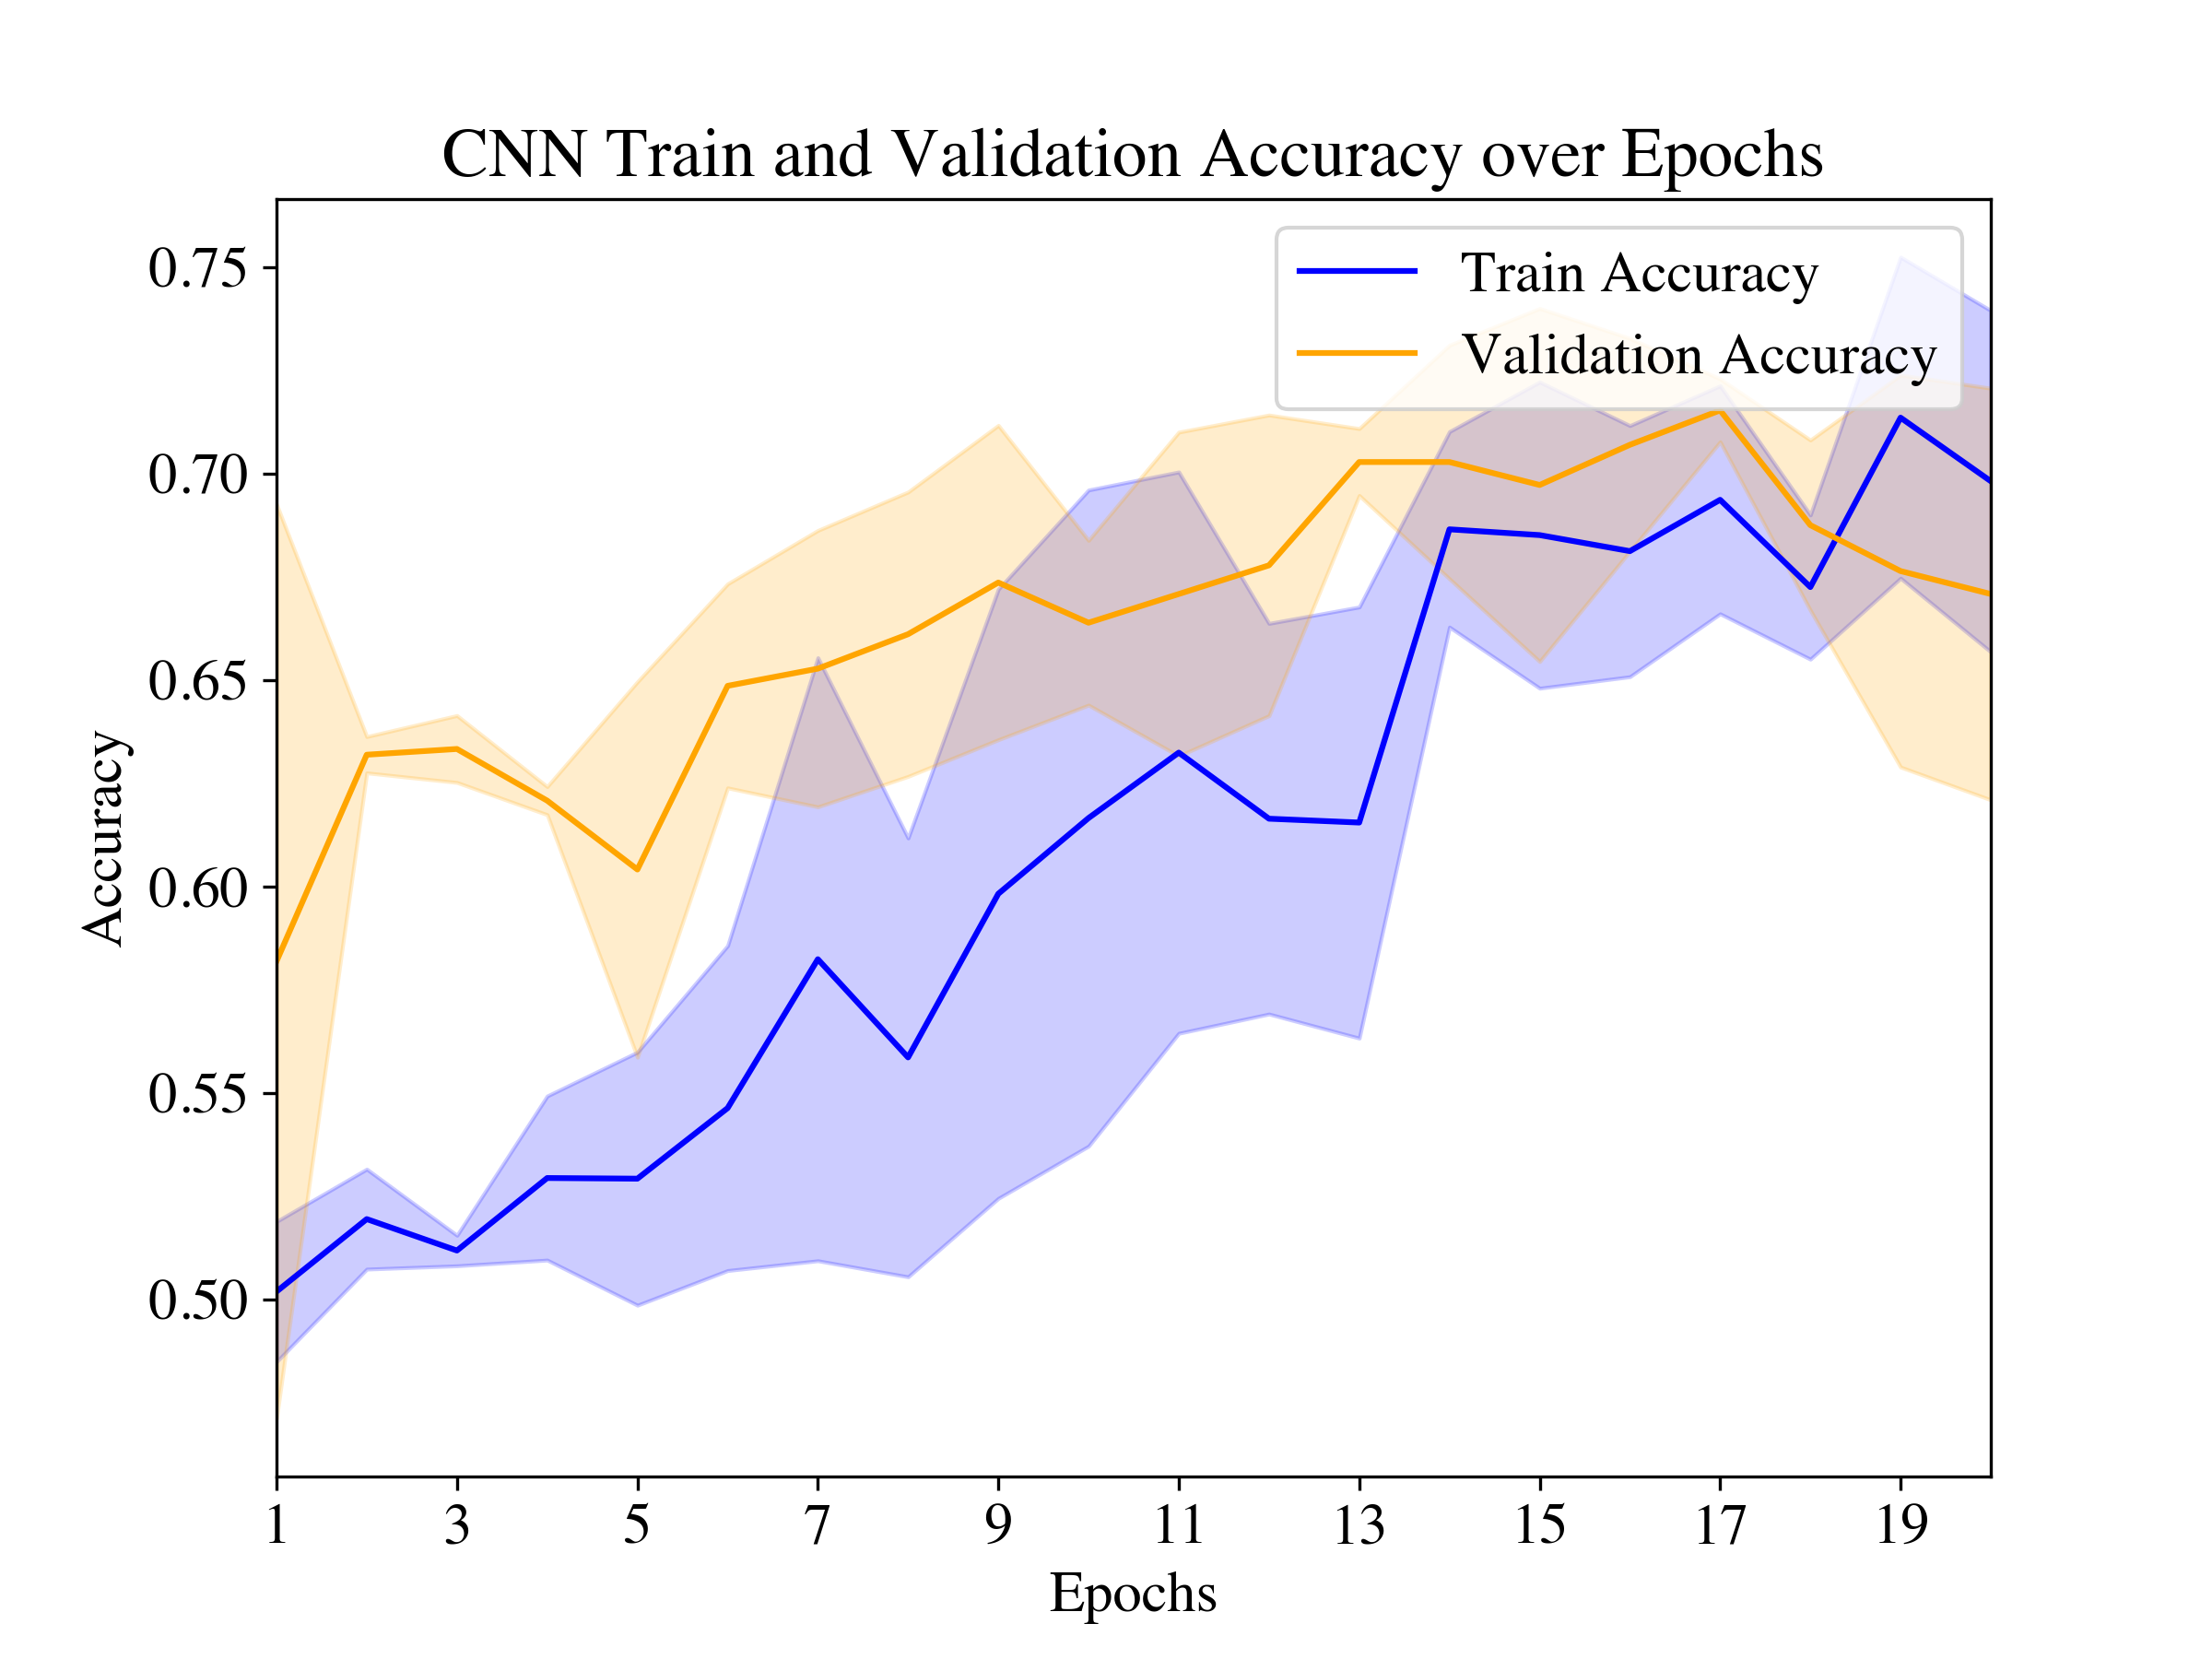
\includegraphics[width=.4\linewidth]{../3d/plots/cnn/accuracy.png}
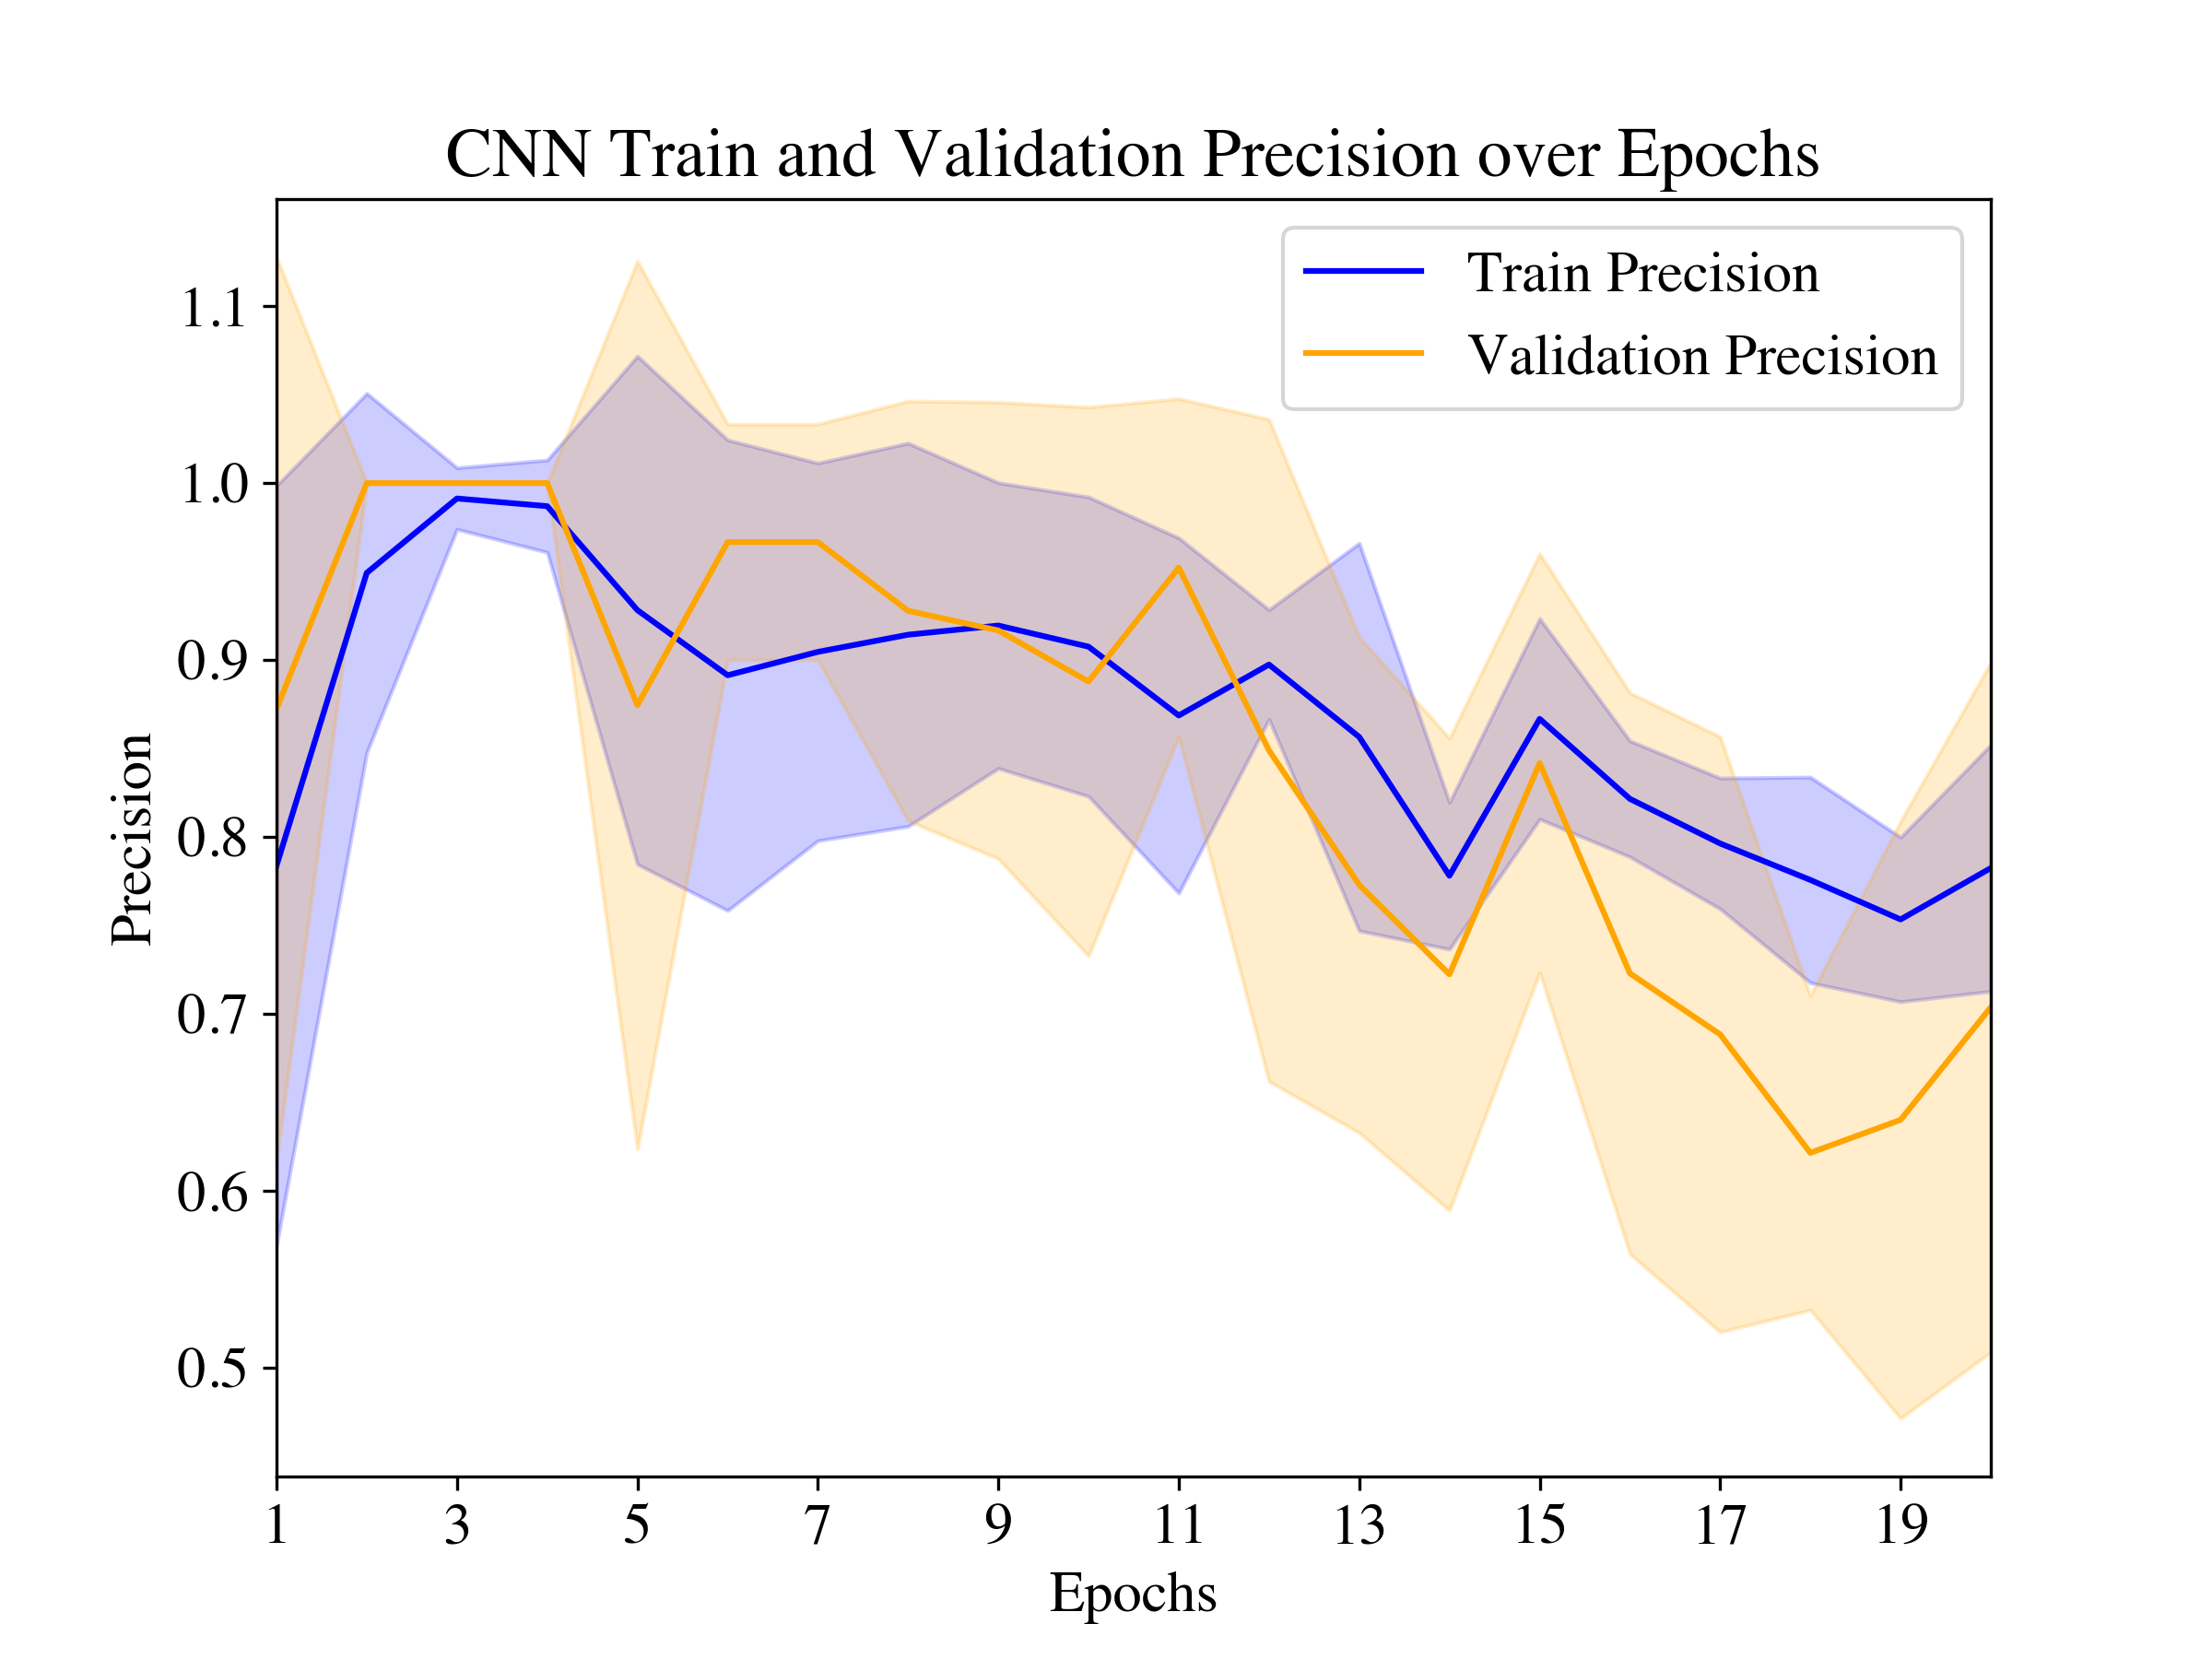
\includegraphics[width=.4\linewidth]{../3d/plots/cnn/precision.png}
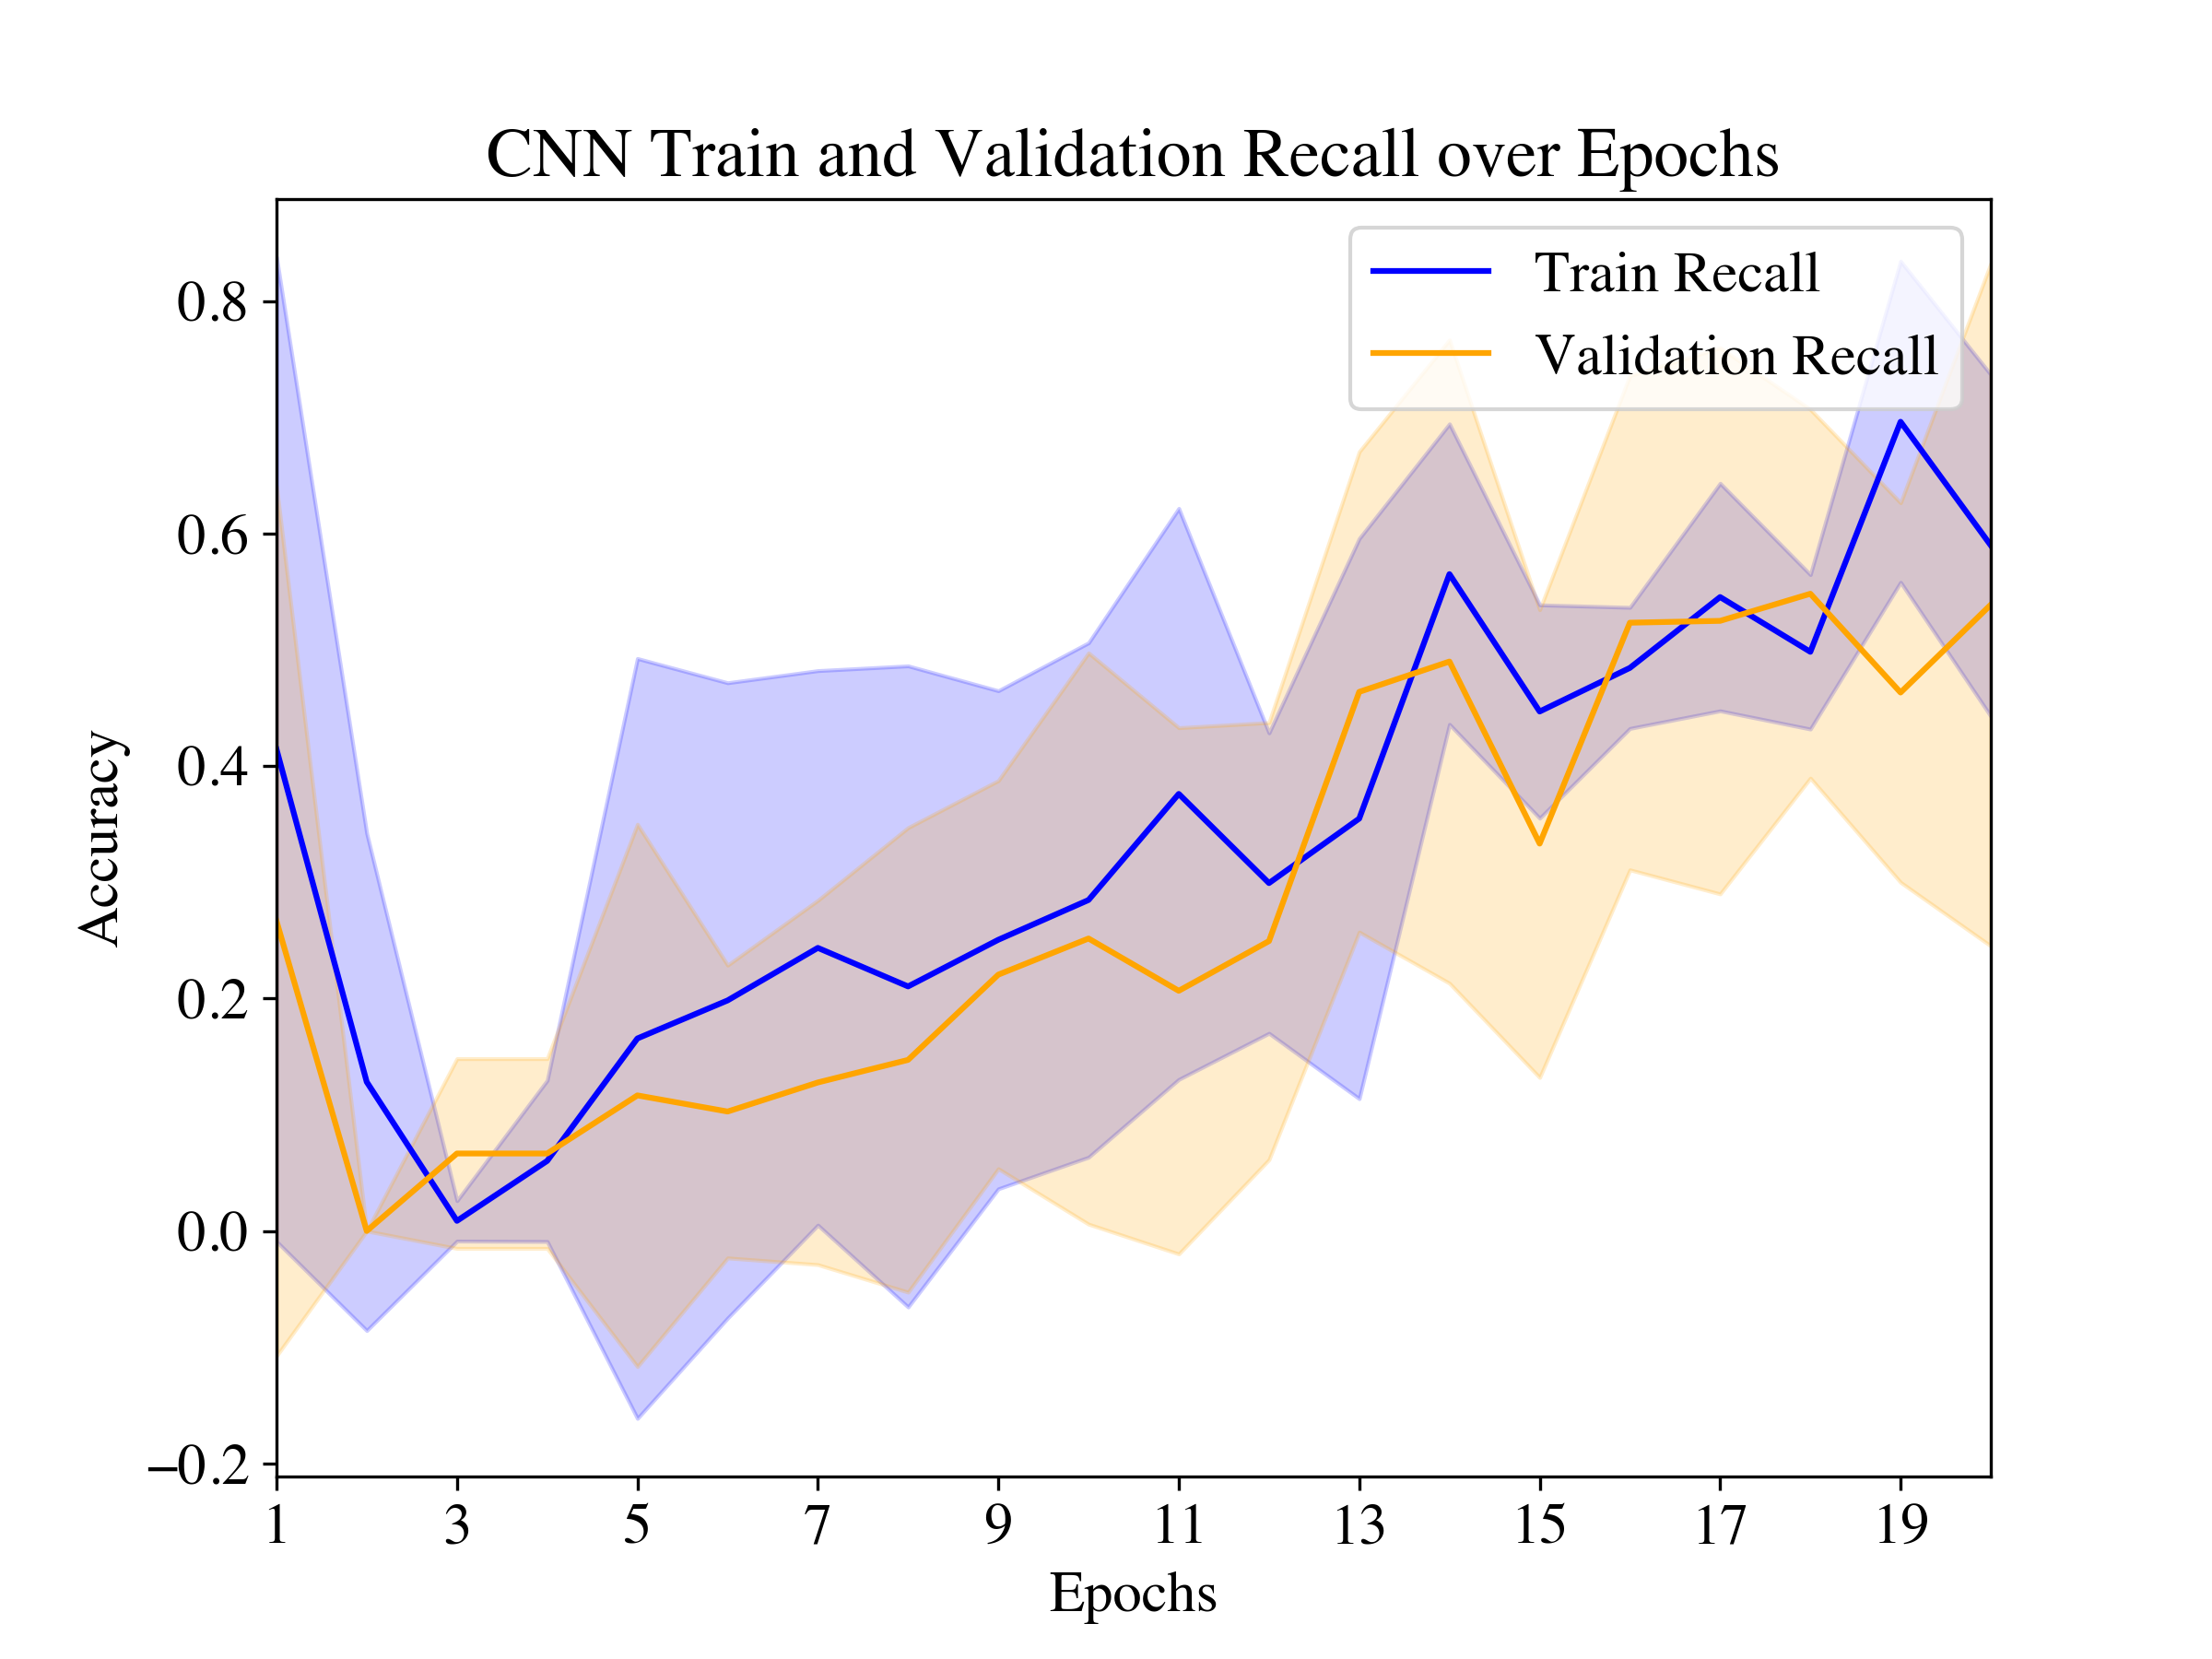
\includegraphics[width=.4\linewidth]{../3d/plots/cnn/recall.png}
\end{center}
\caption{Vanilla train (blue) and validation (orange) loss curve (top left), accuracy curve (top right) precision curve (bottom left) validation curve (bottom right) with mean and standard deviation. This model was trained on the concatenated Retina Layer d, r, s.}
\end{figure}

\begin{figure}[h]
\begin{center}
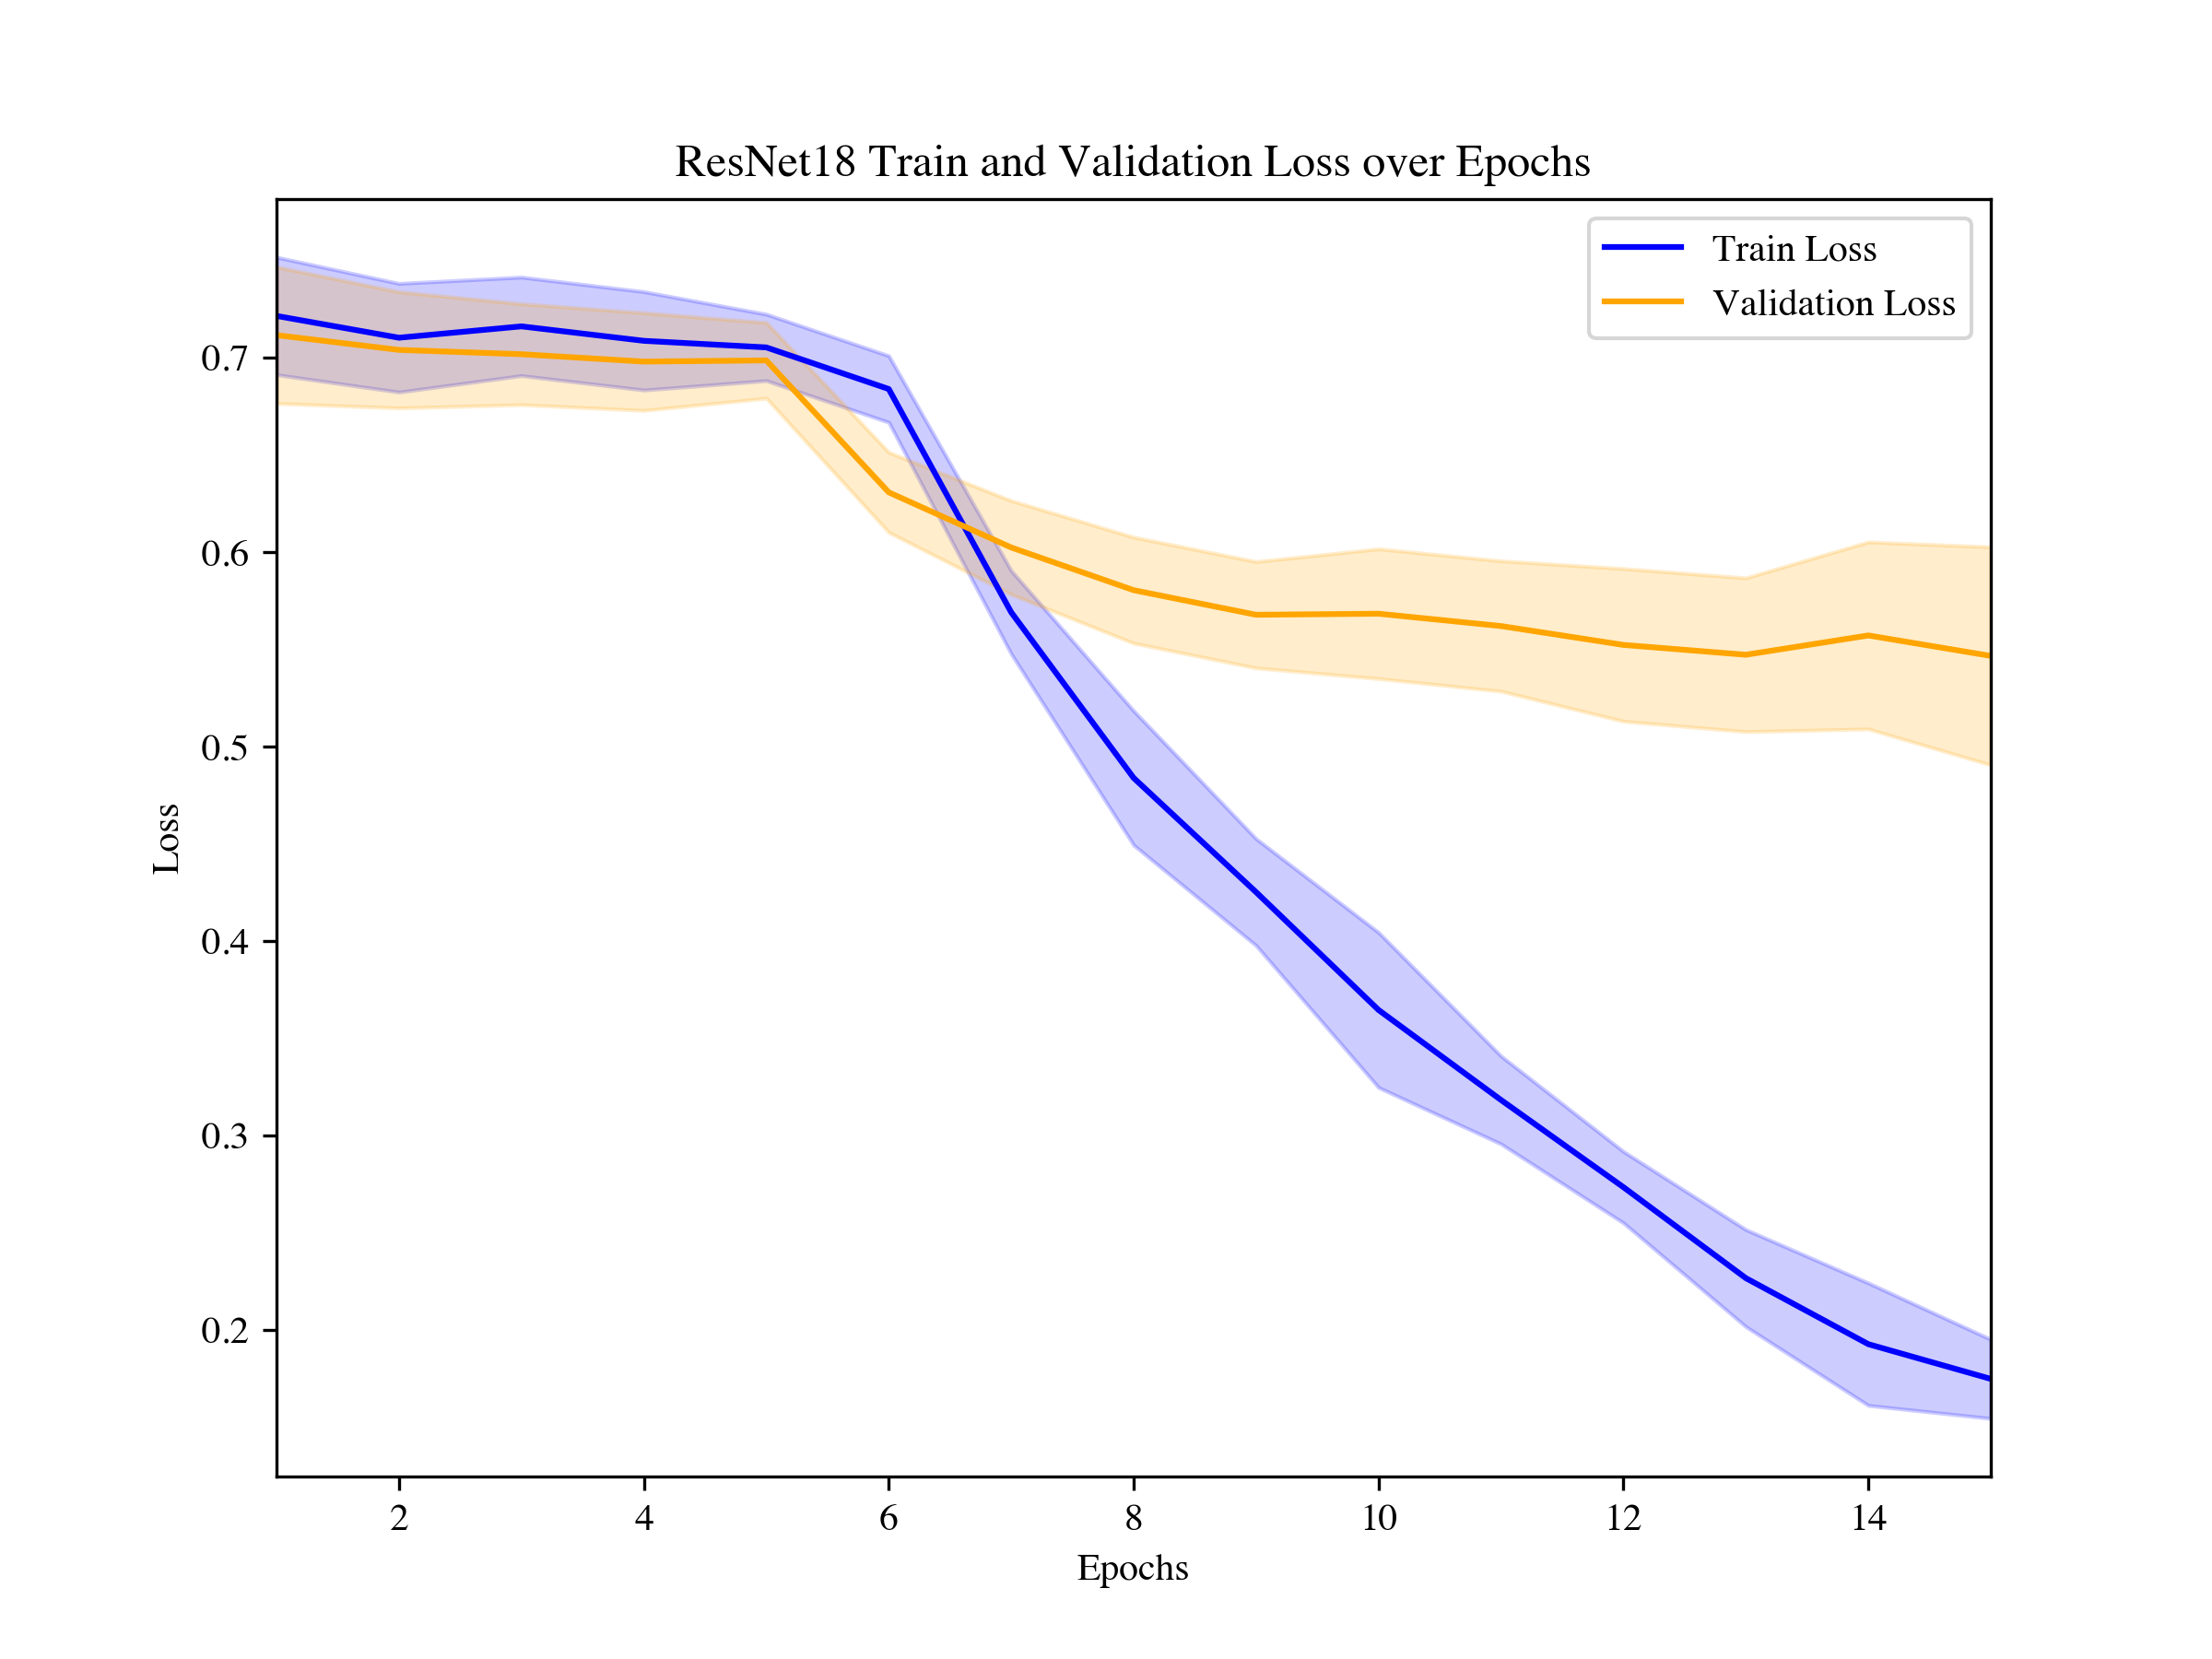
\includegraphics[width=.4\linewidth]{../3d/plots/resnet18/loss.png}
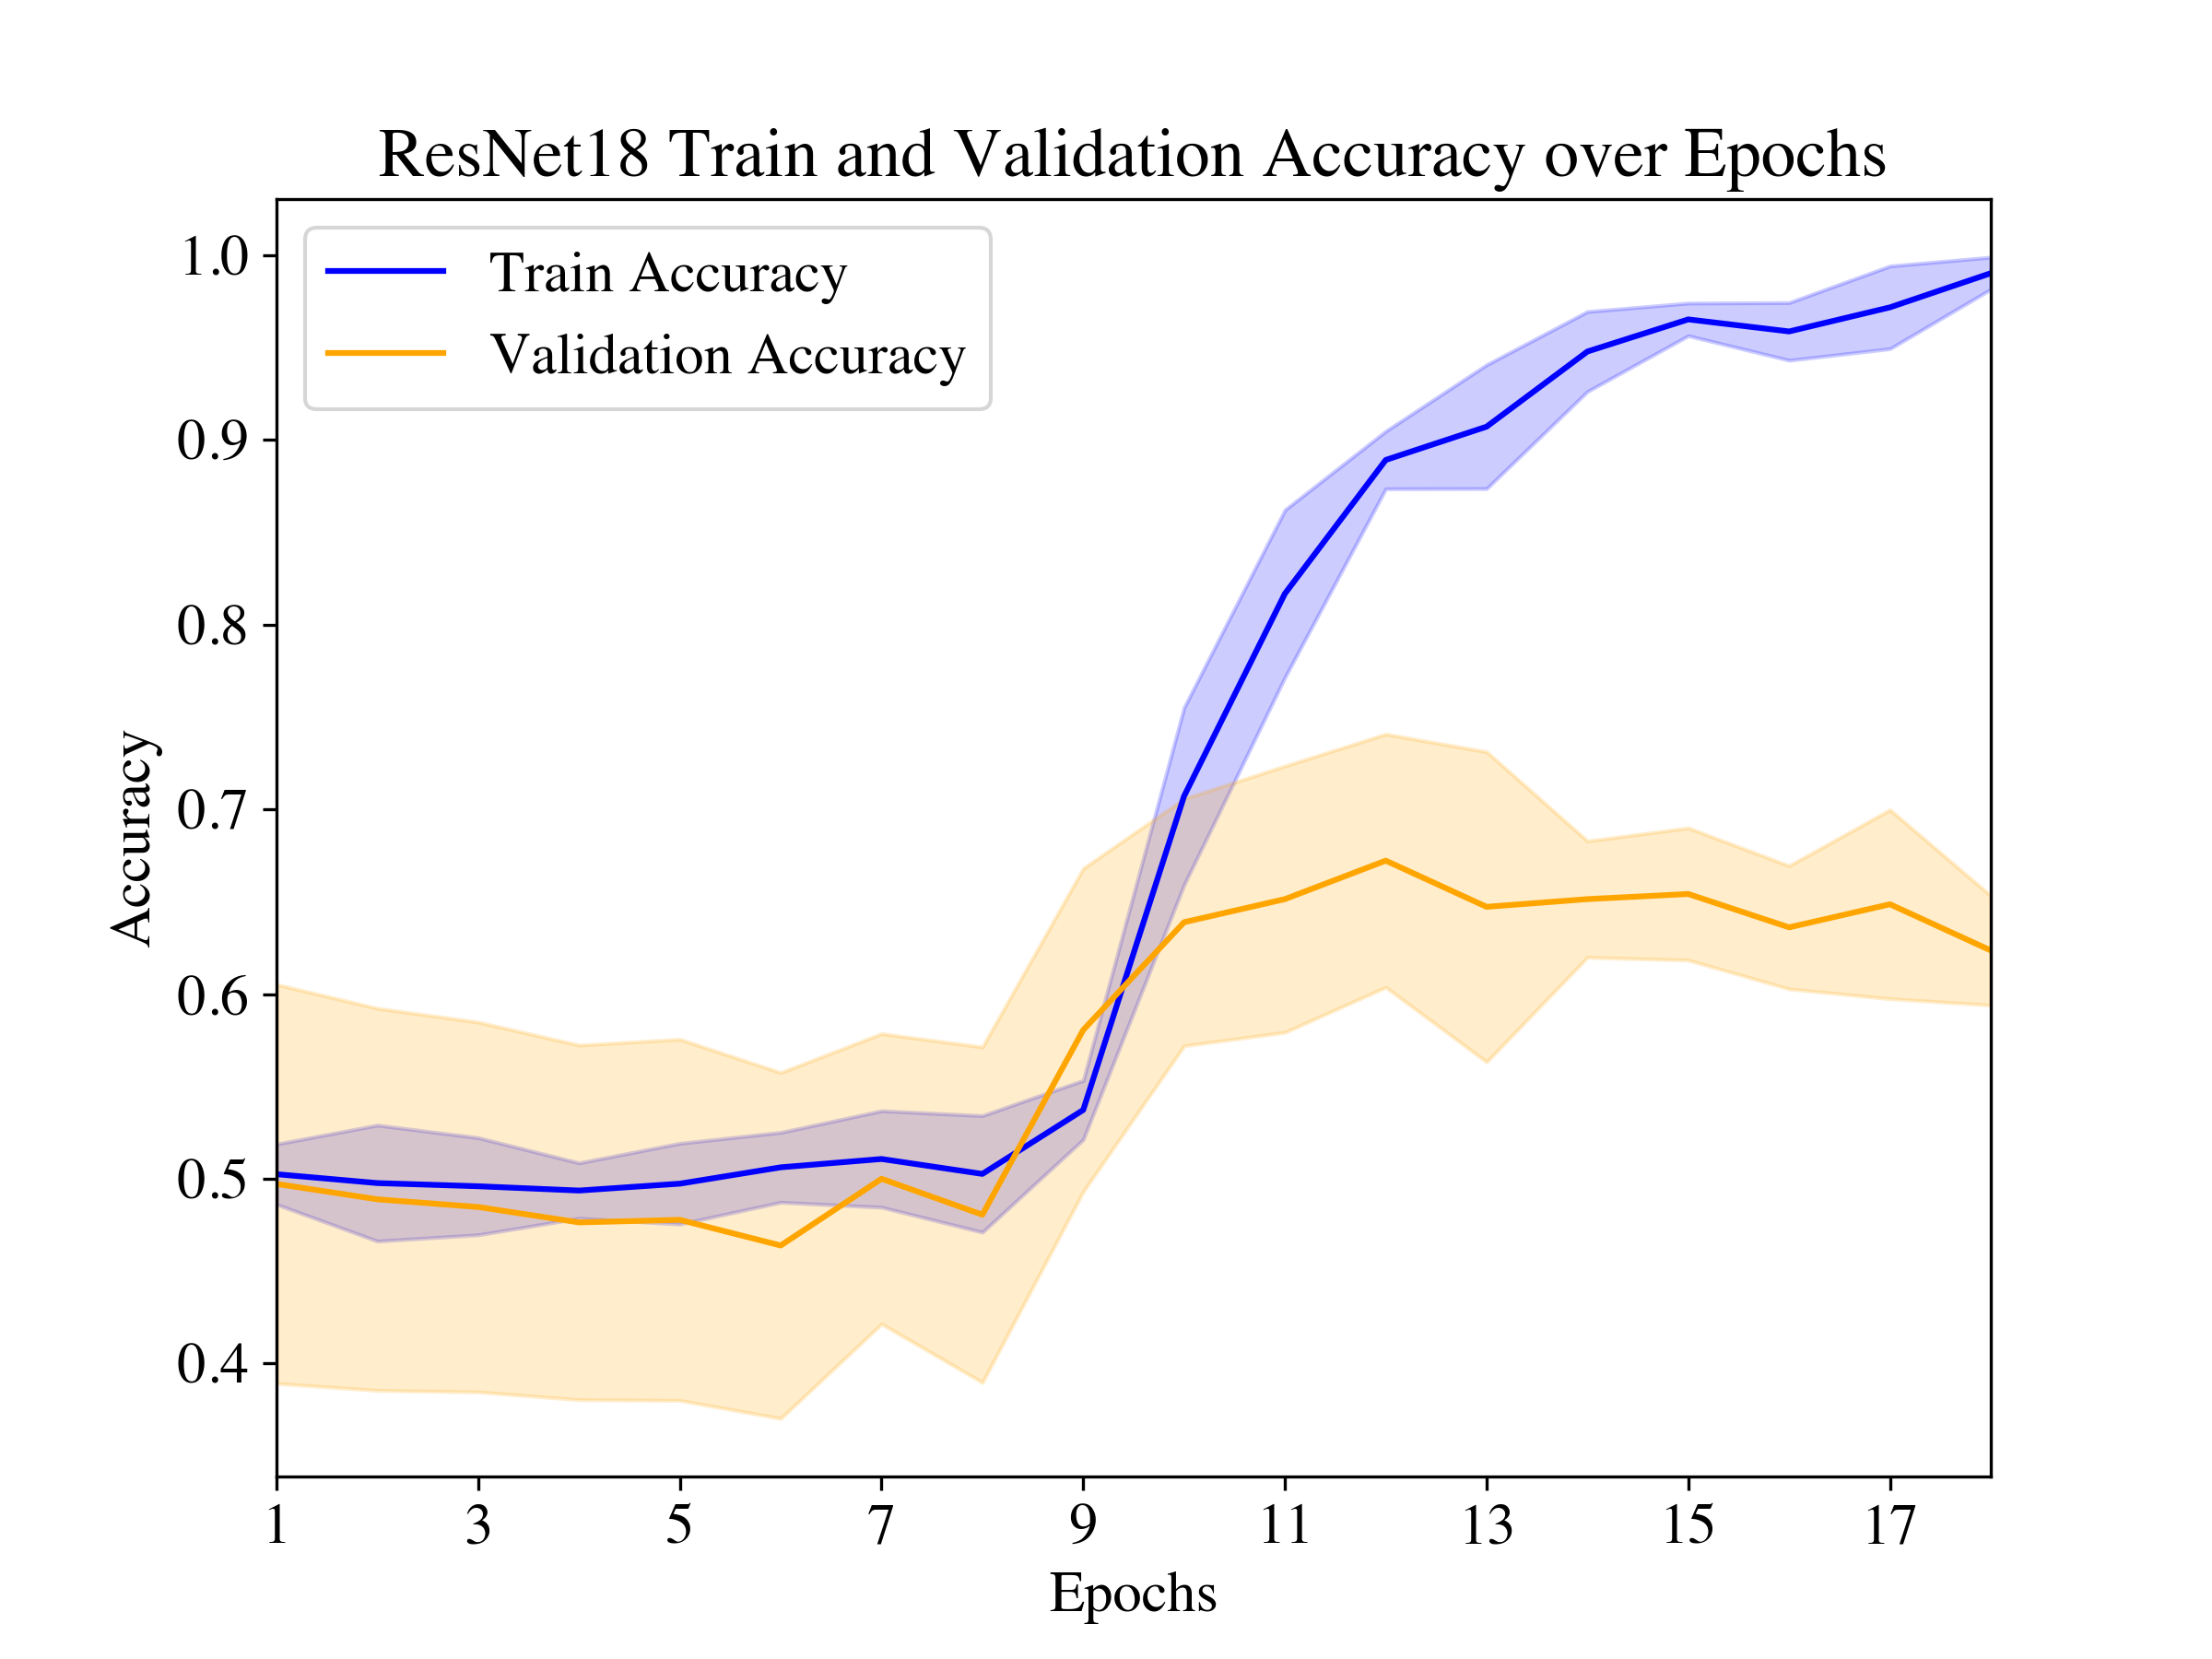
\includegraphics[width=.4\linewidth]{../3d/plots/resnet18/accuracy.png}
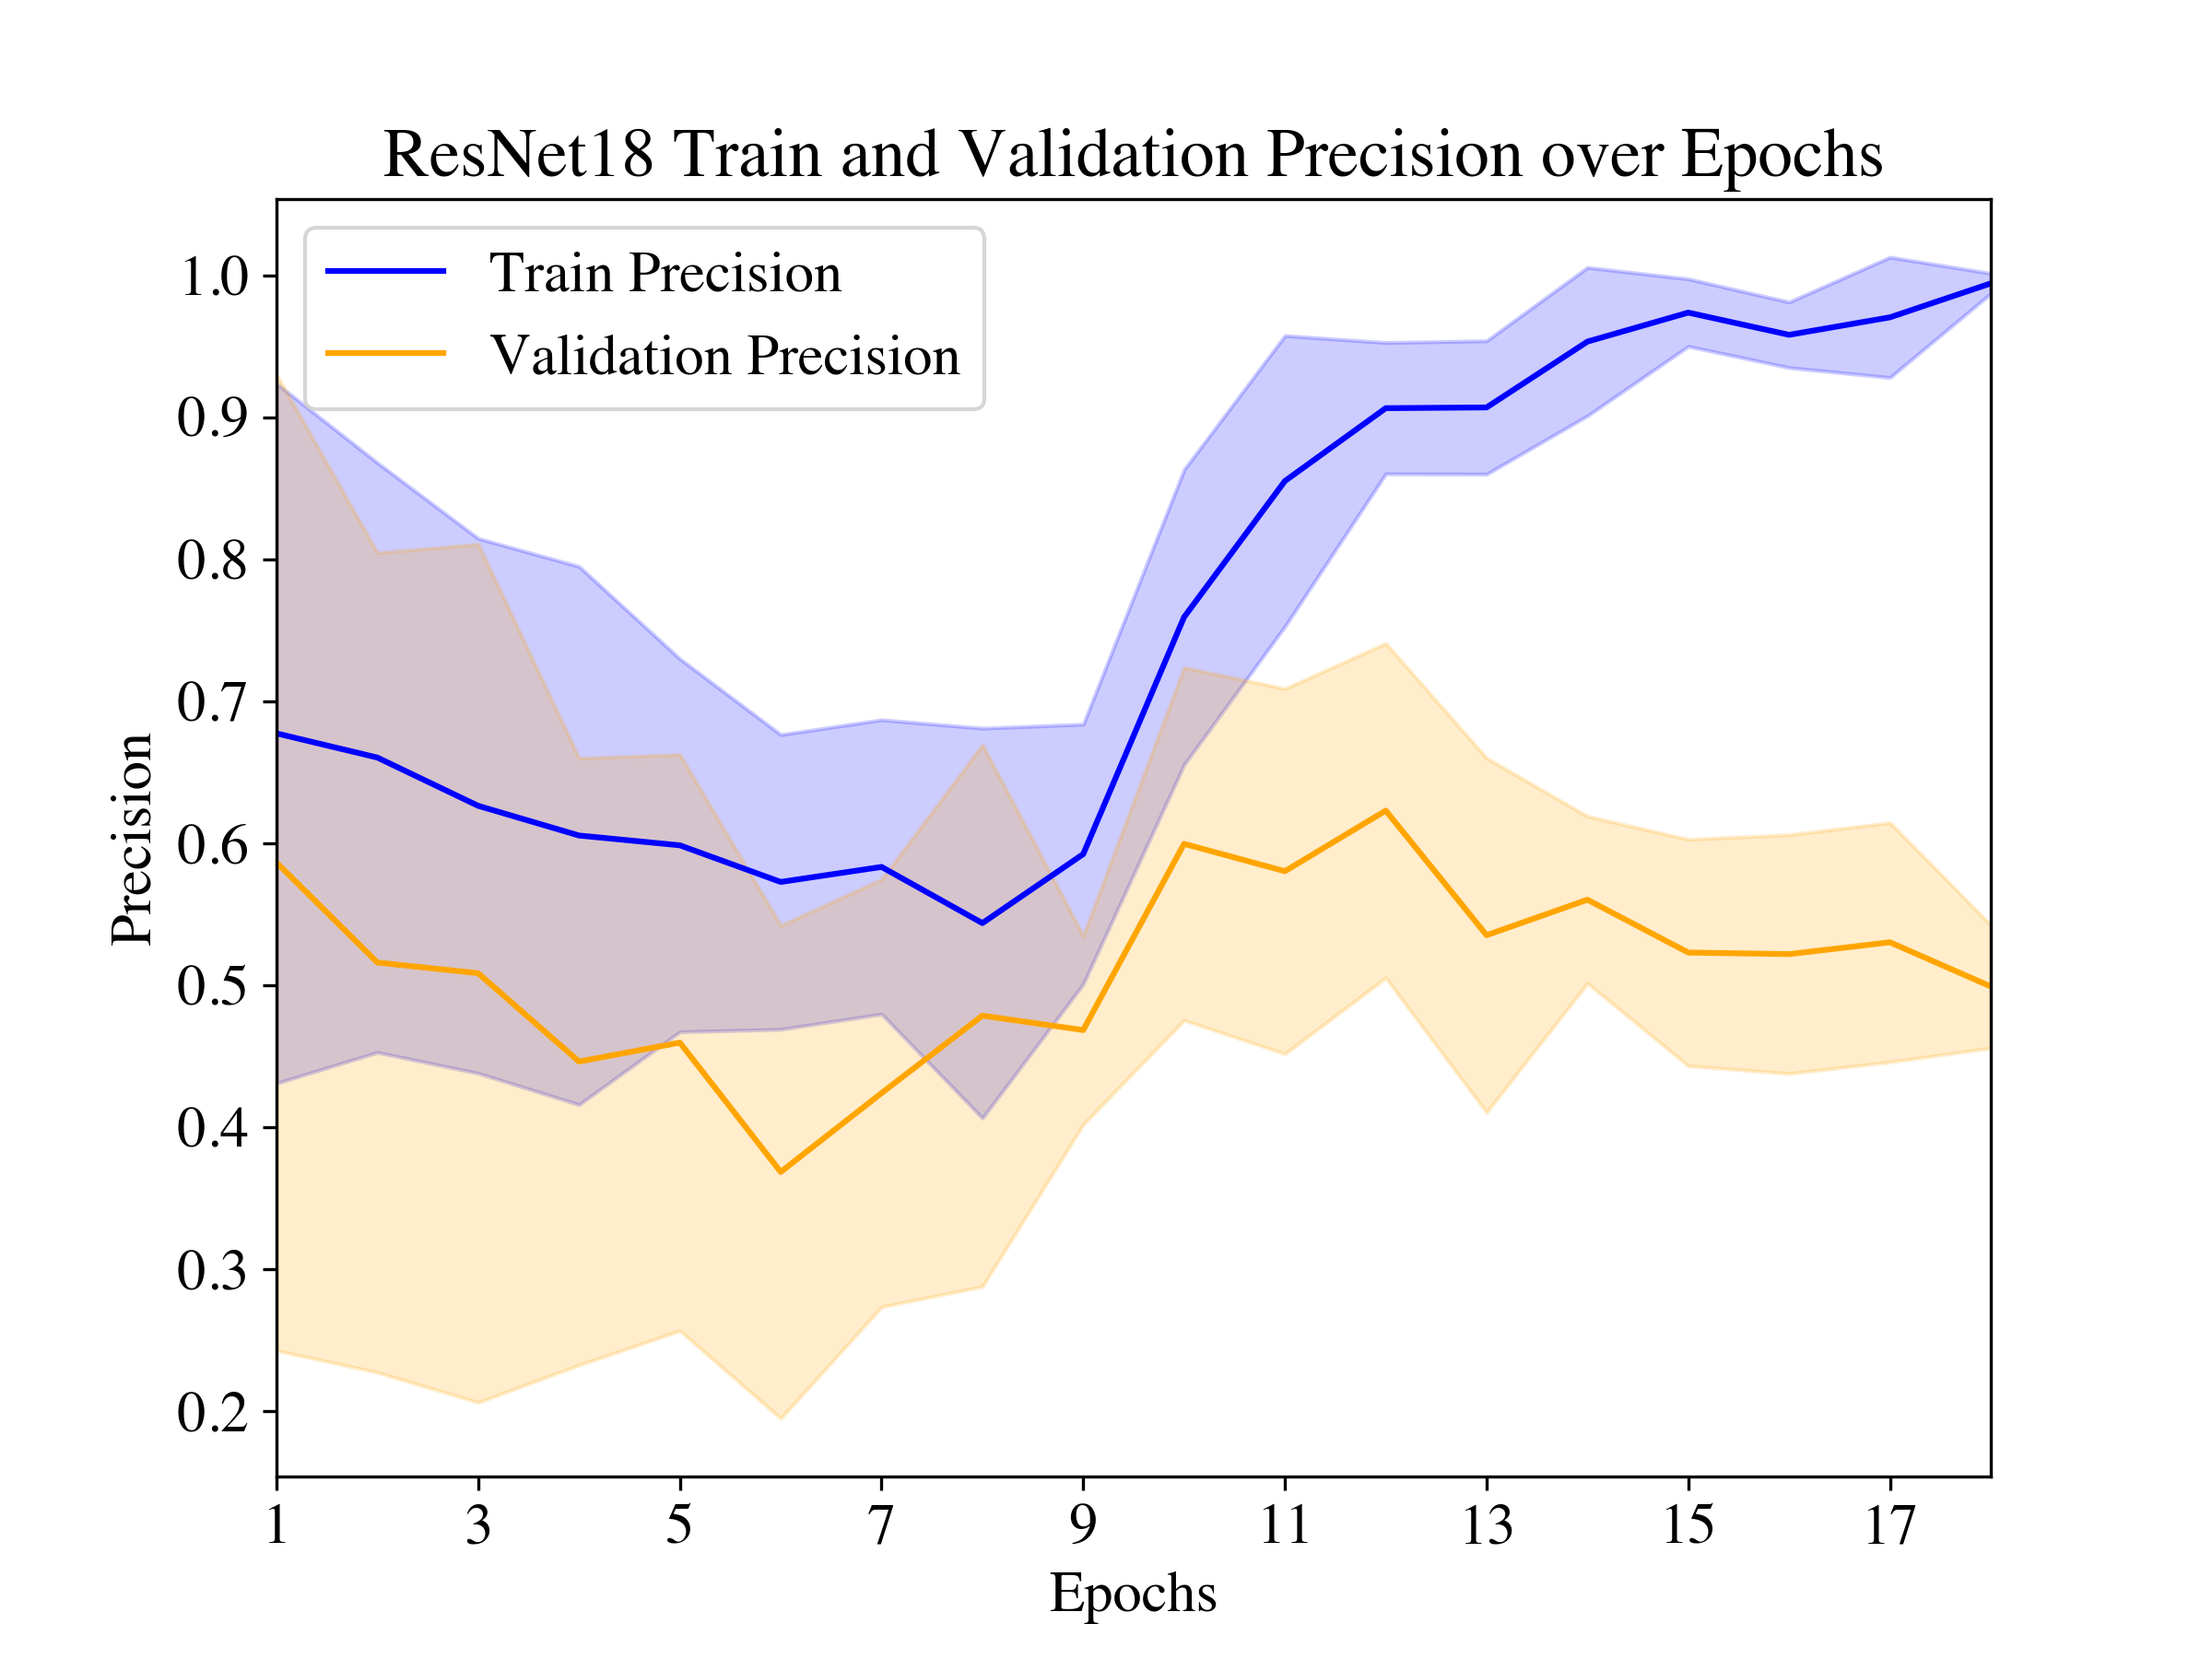
\includegraphics[width=.4\linewidth]{../3d/plots/resnet18/precision_score.png}
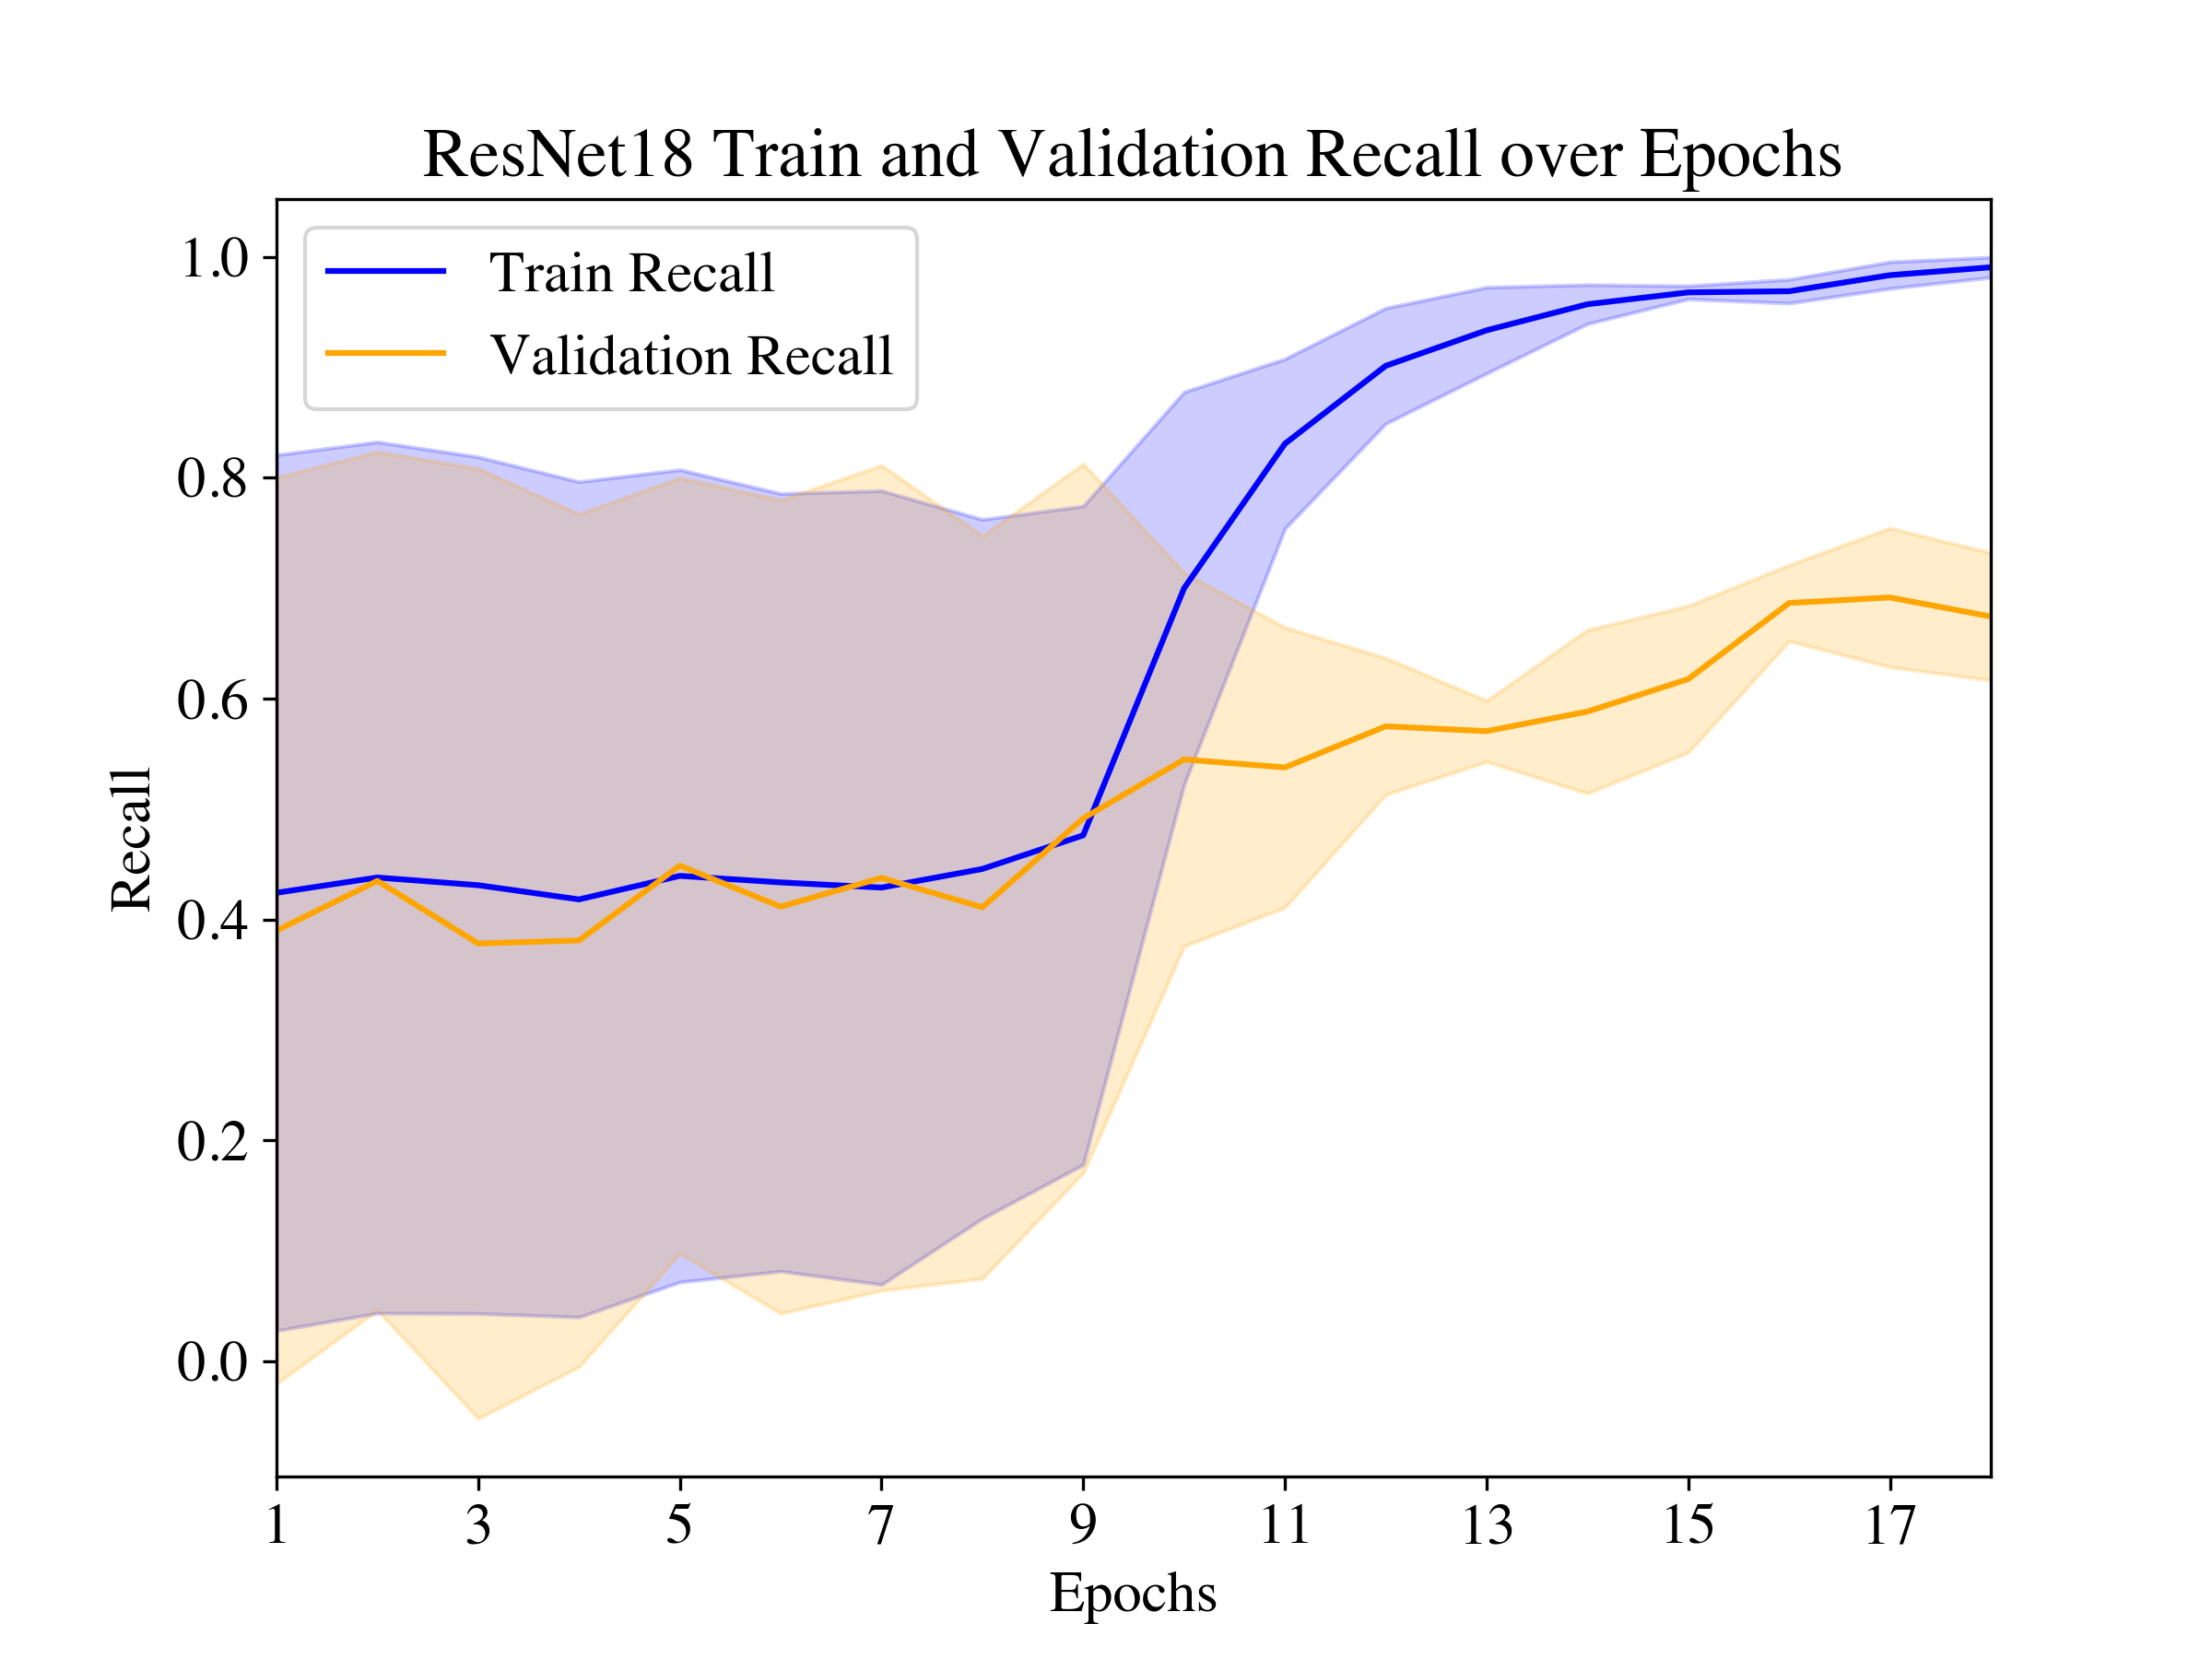
\includegraphics[width=.4\linewidth]{../3d/plots/resnet18/recall_score.png}
\end{center}
\caption{ResNet18 train (blue) and validation (orange) loss curve (top left), accuracy curve (top right) precision curve (bottom left) validation curve (bottom right) with mean and standard deviation. This model was trained on the concatenated Retina Layer d, r, s.}
\end{figure}
\begin{figure}[h]
\begin{center}
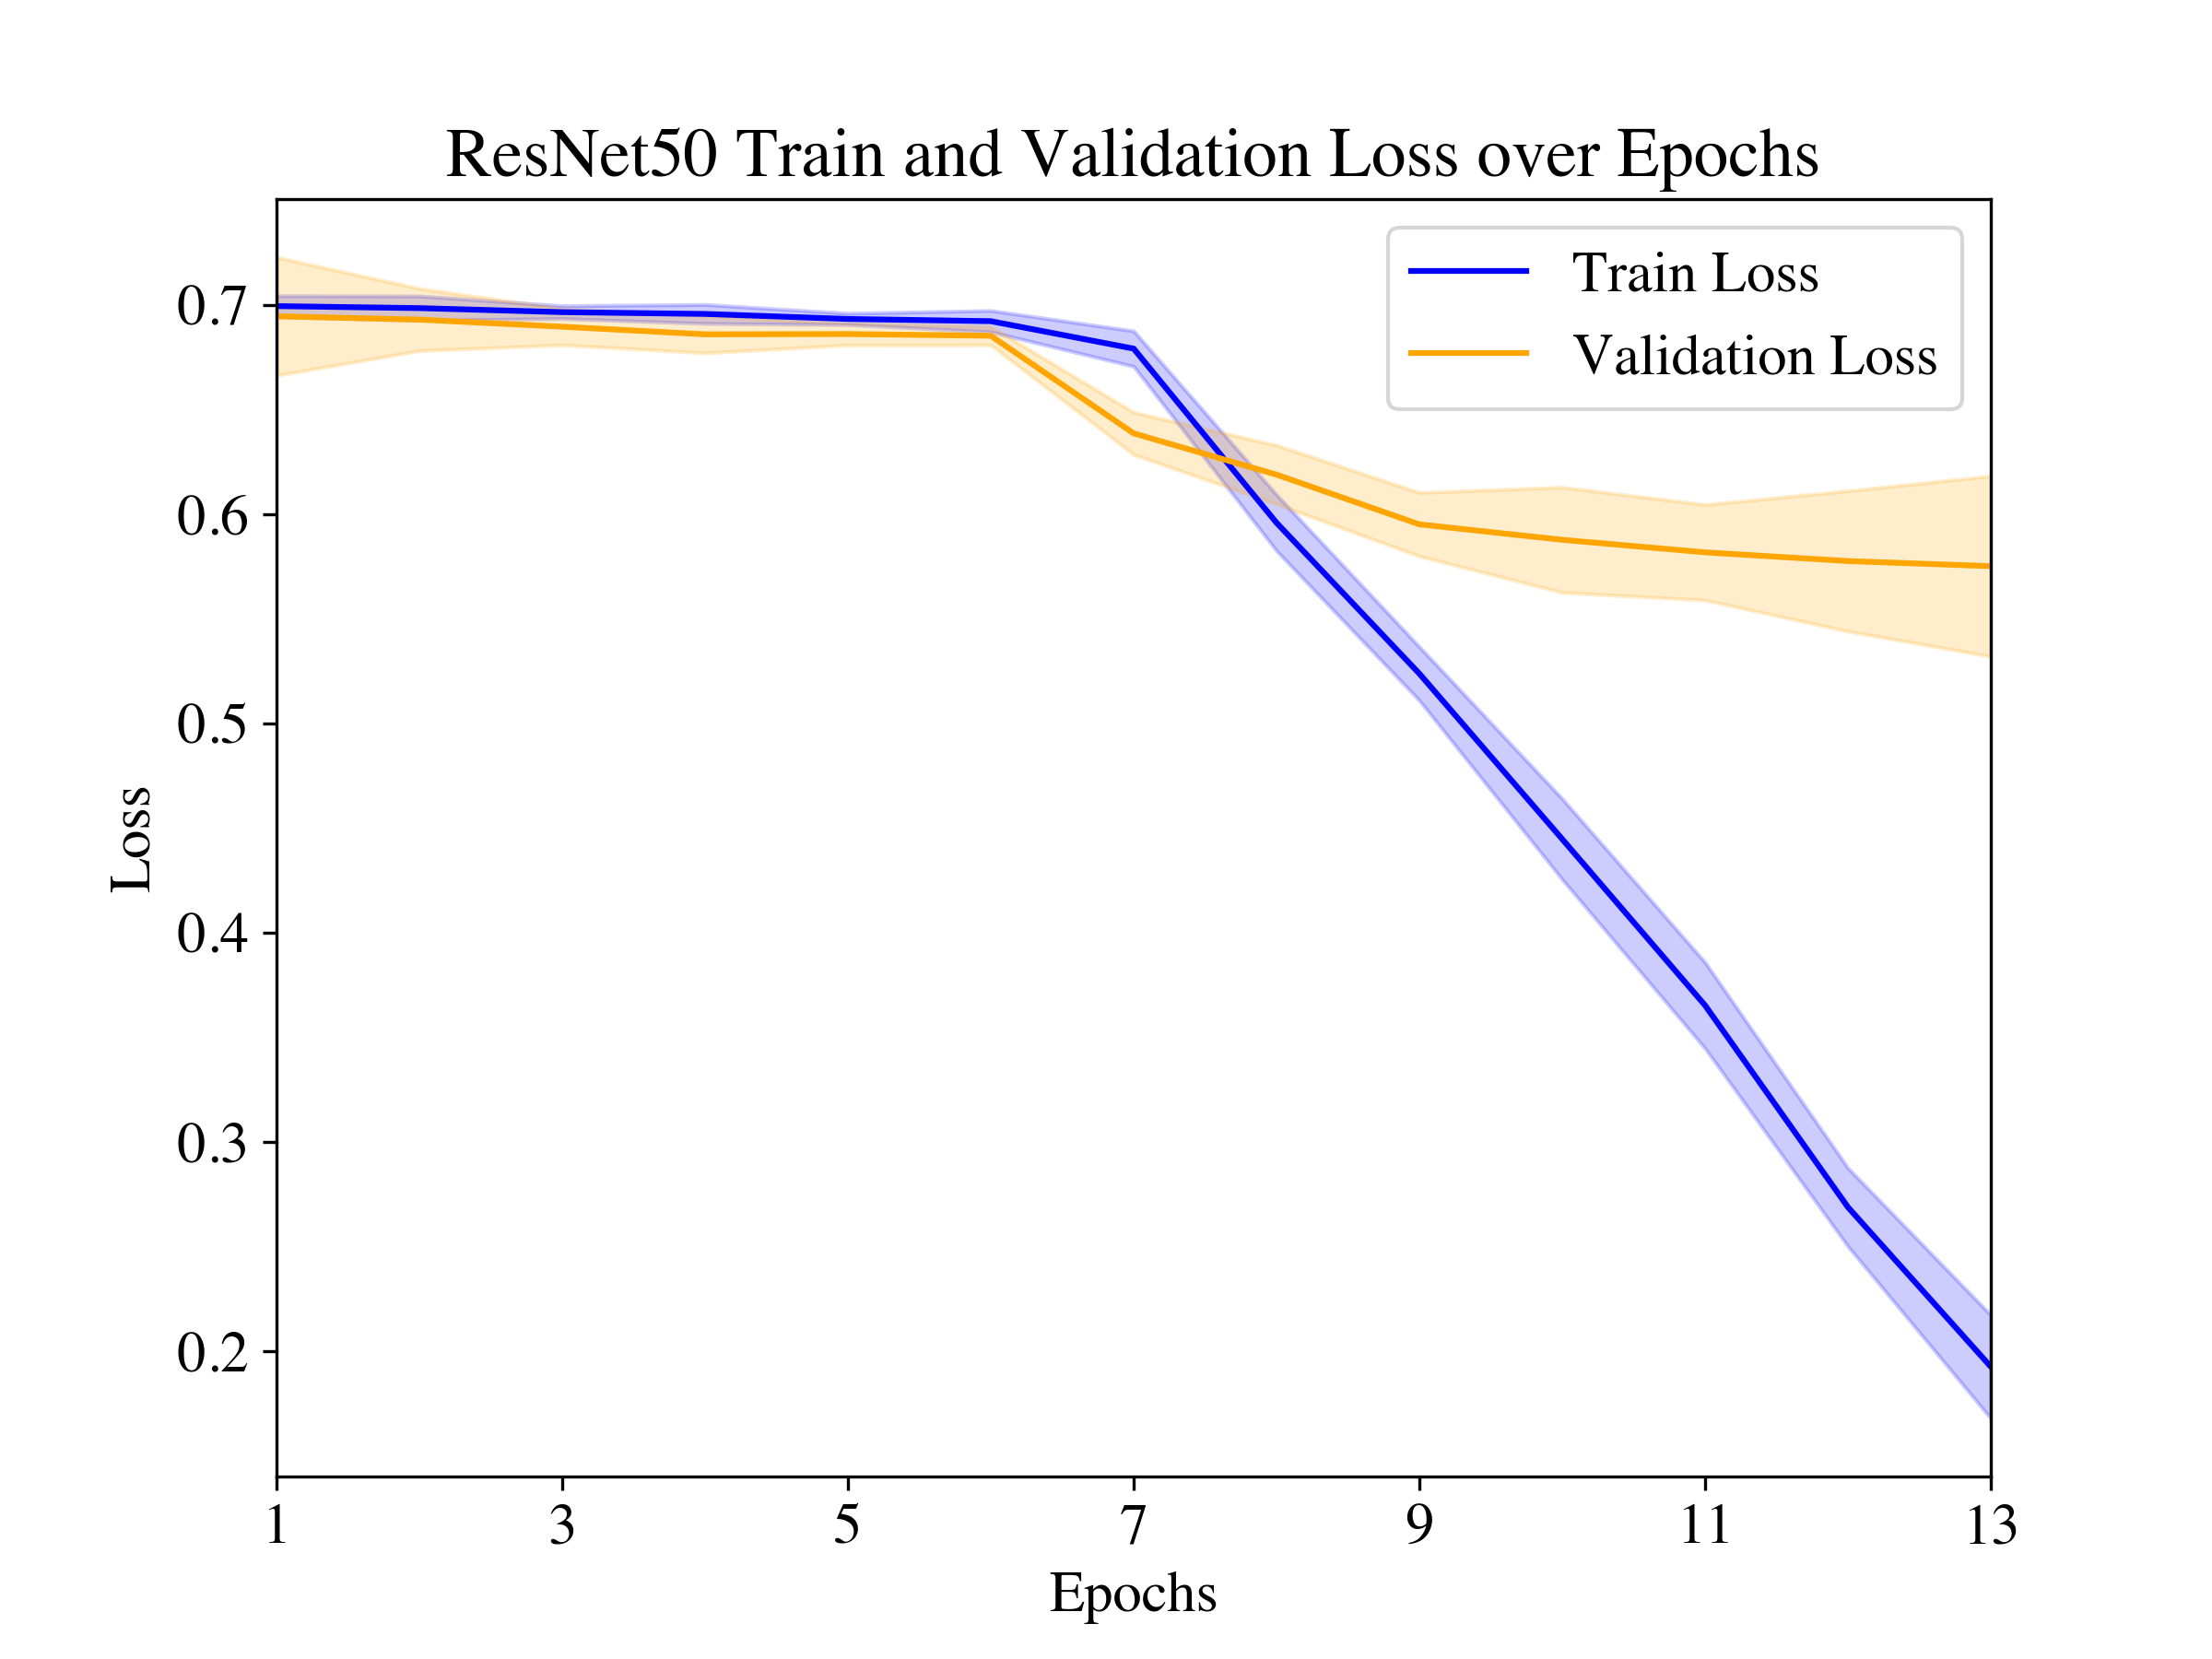
\includegraphics[width=.4\linewidth]{../3d/plots/resnet50/loss.png}
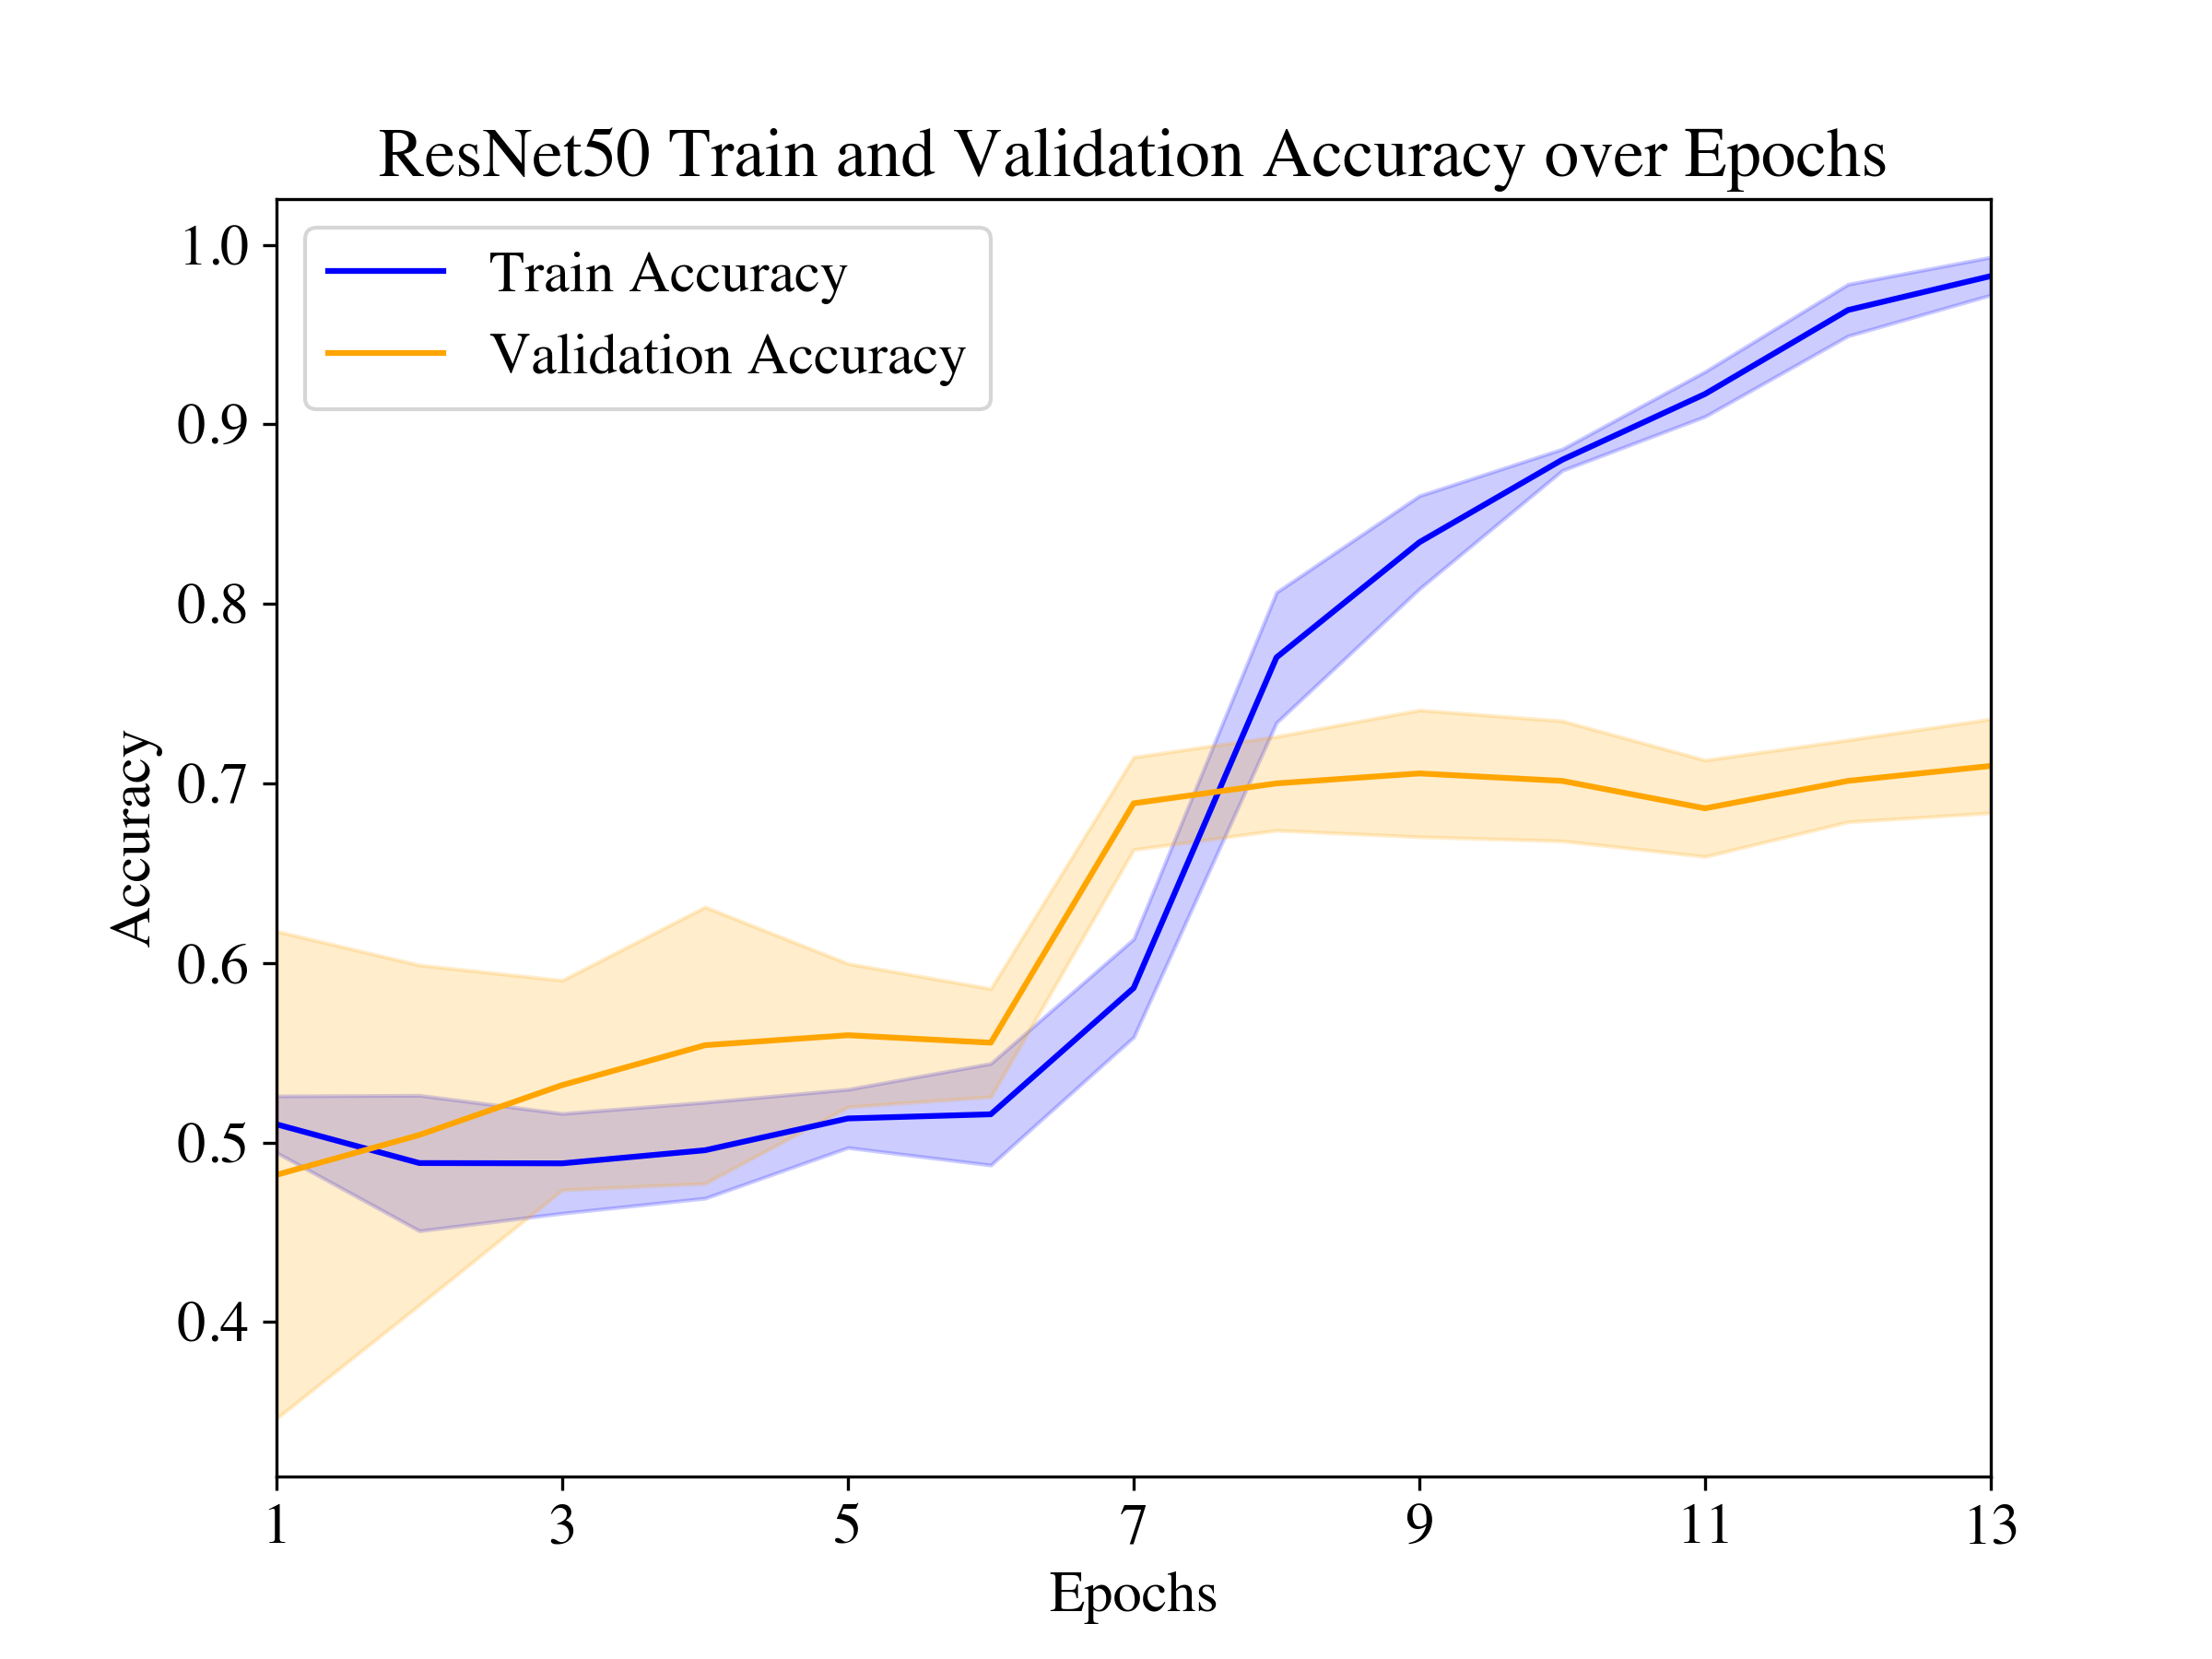
\includegraphics[width=.4\linewidth]{../3d/plots/resnet50/accuracy.png}
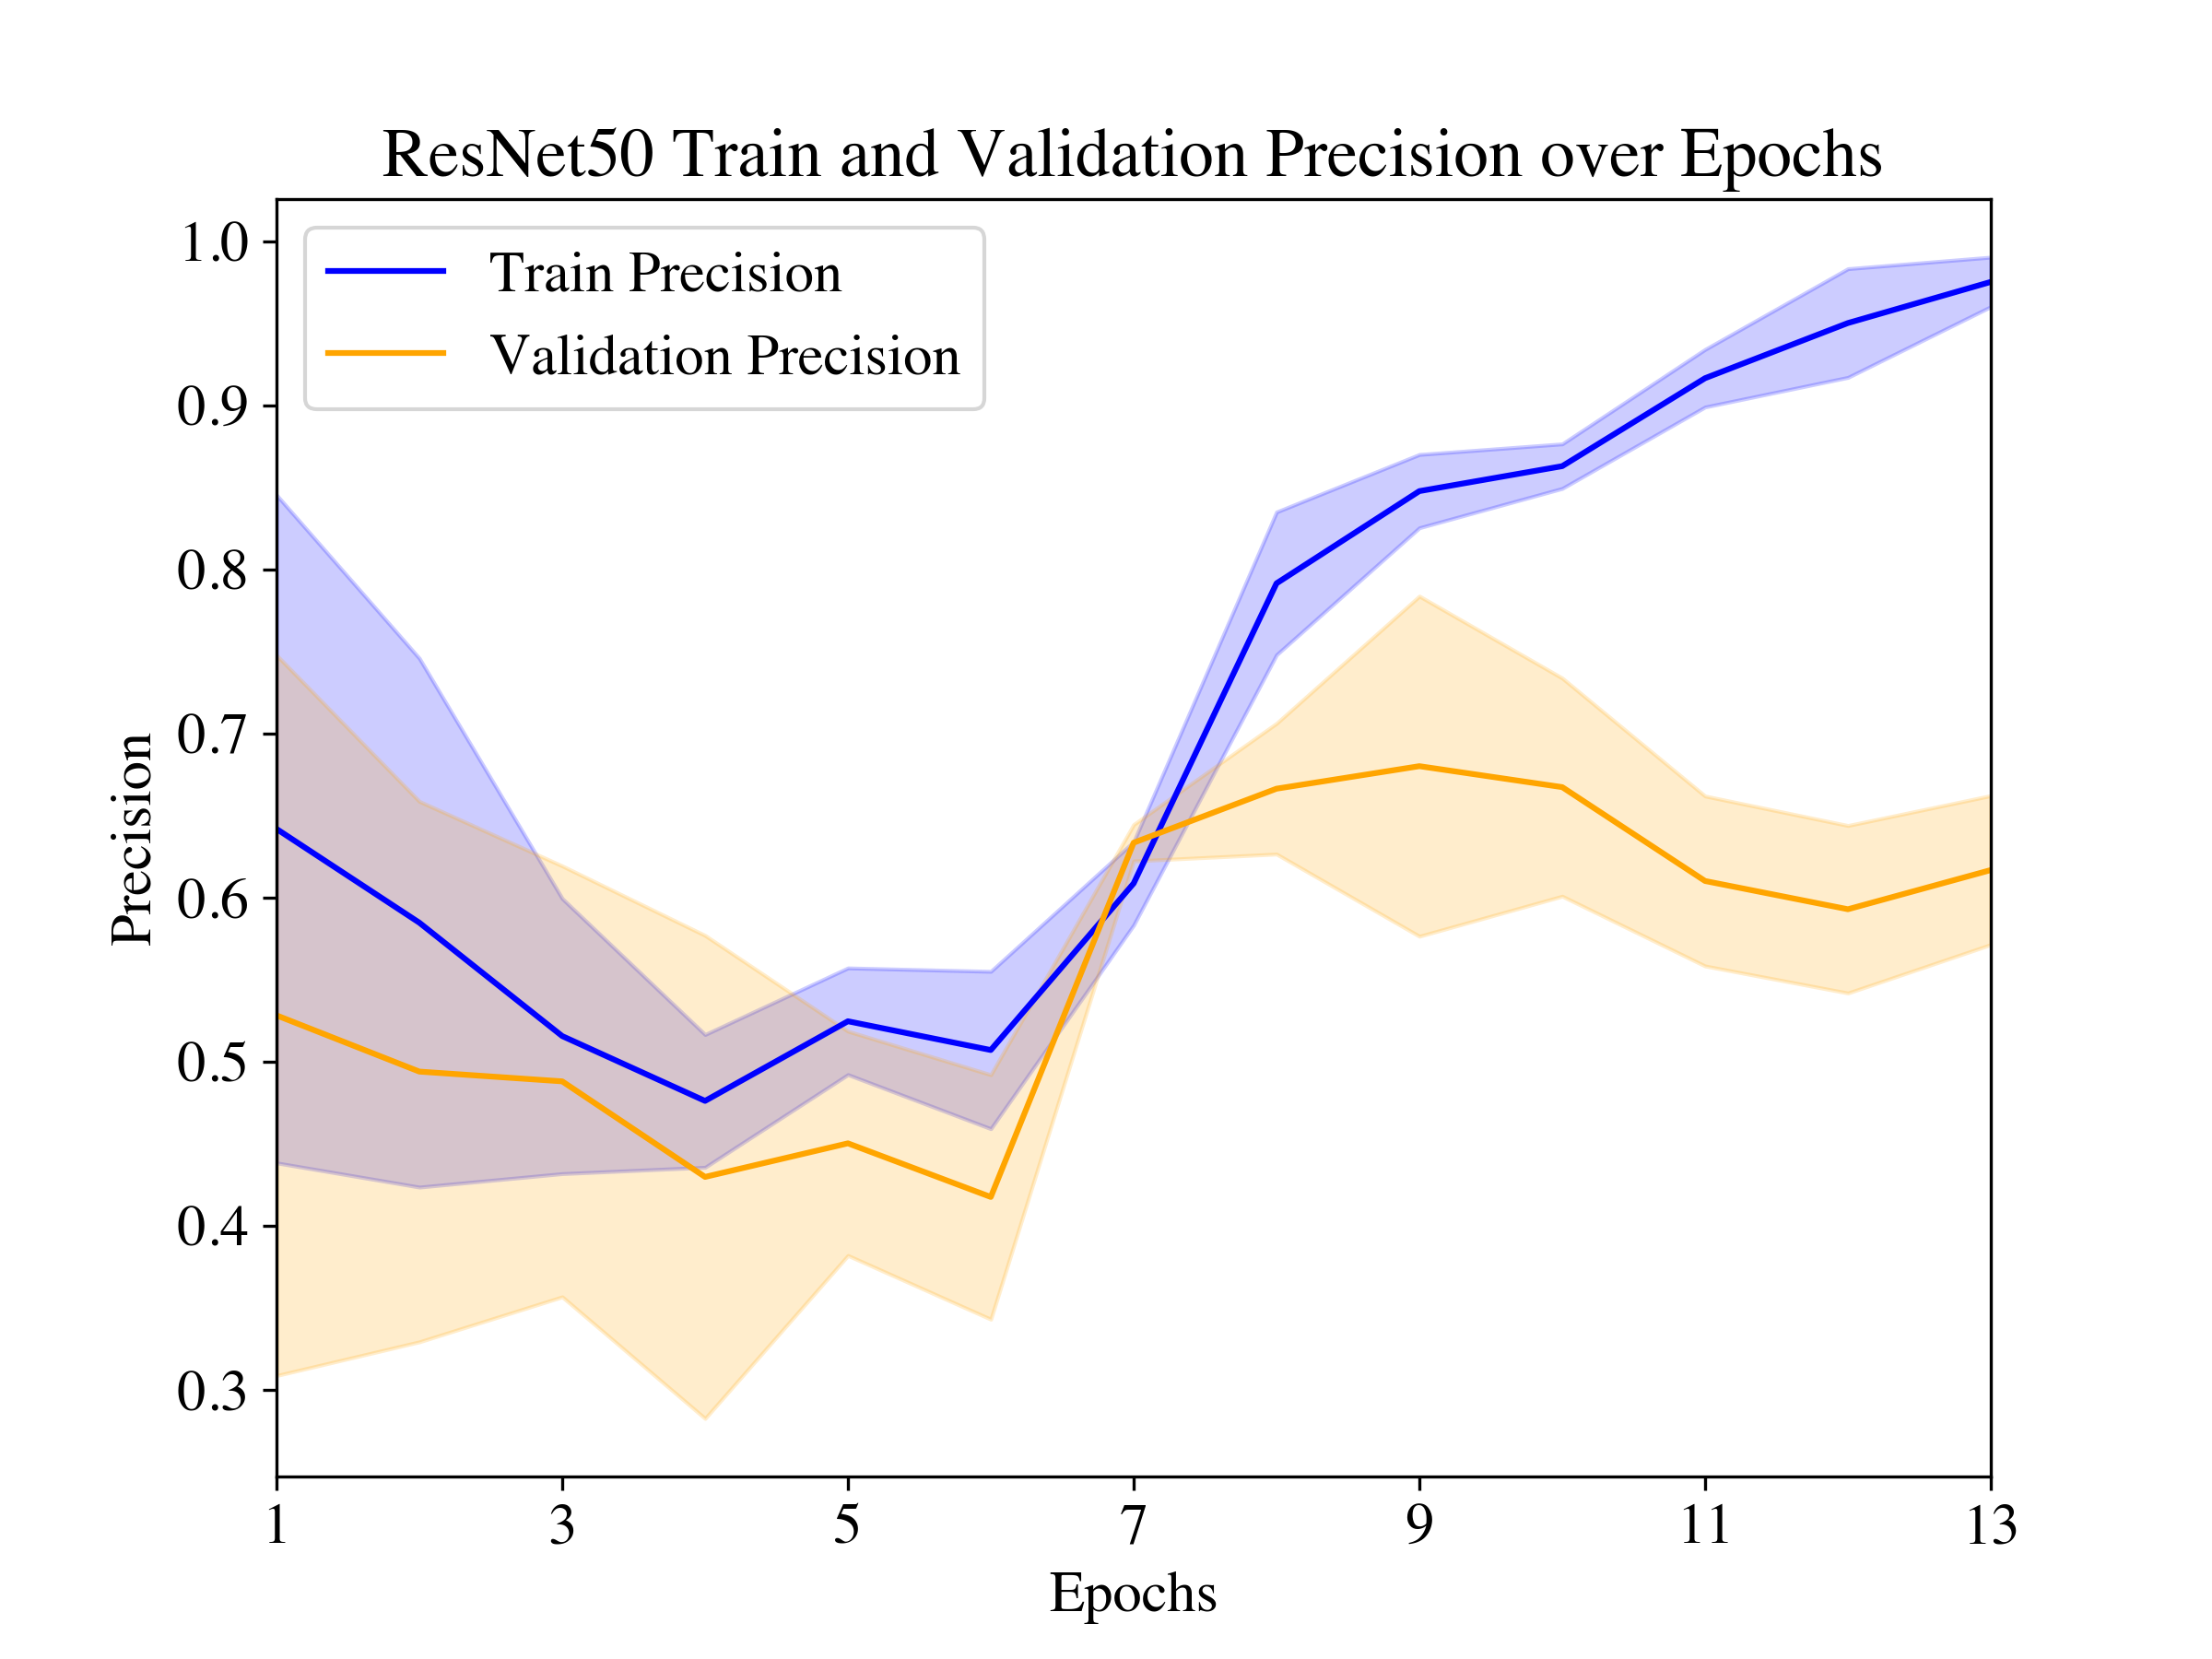
\includegraphics[width=.4\linewidth]{../3d/plots/resnet50/precision.png}
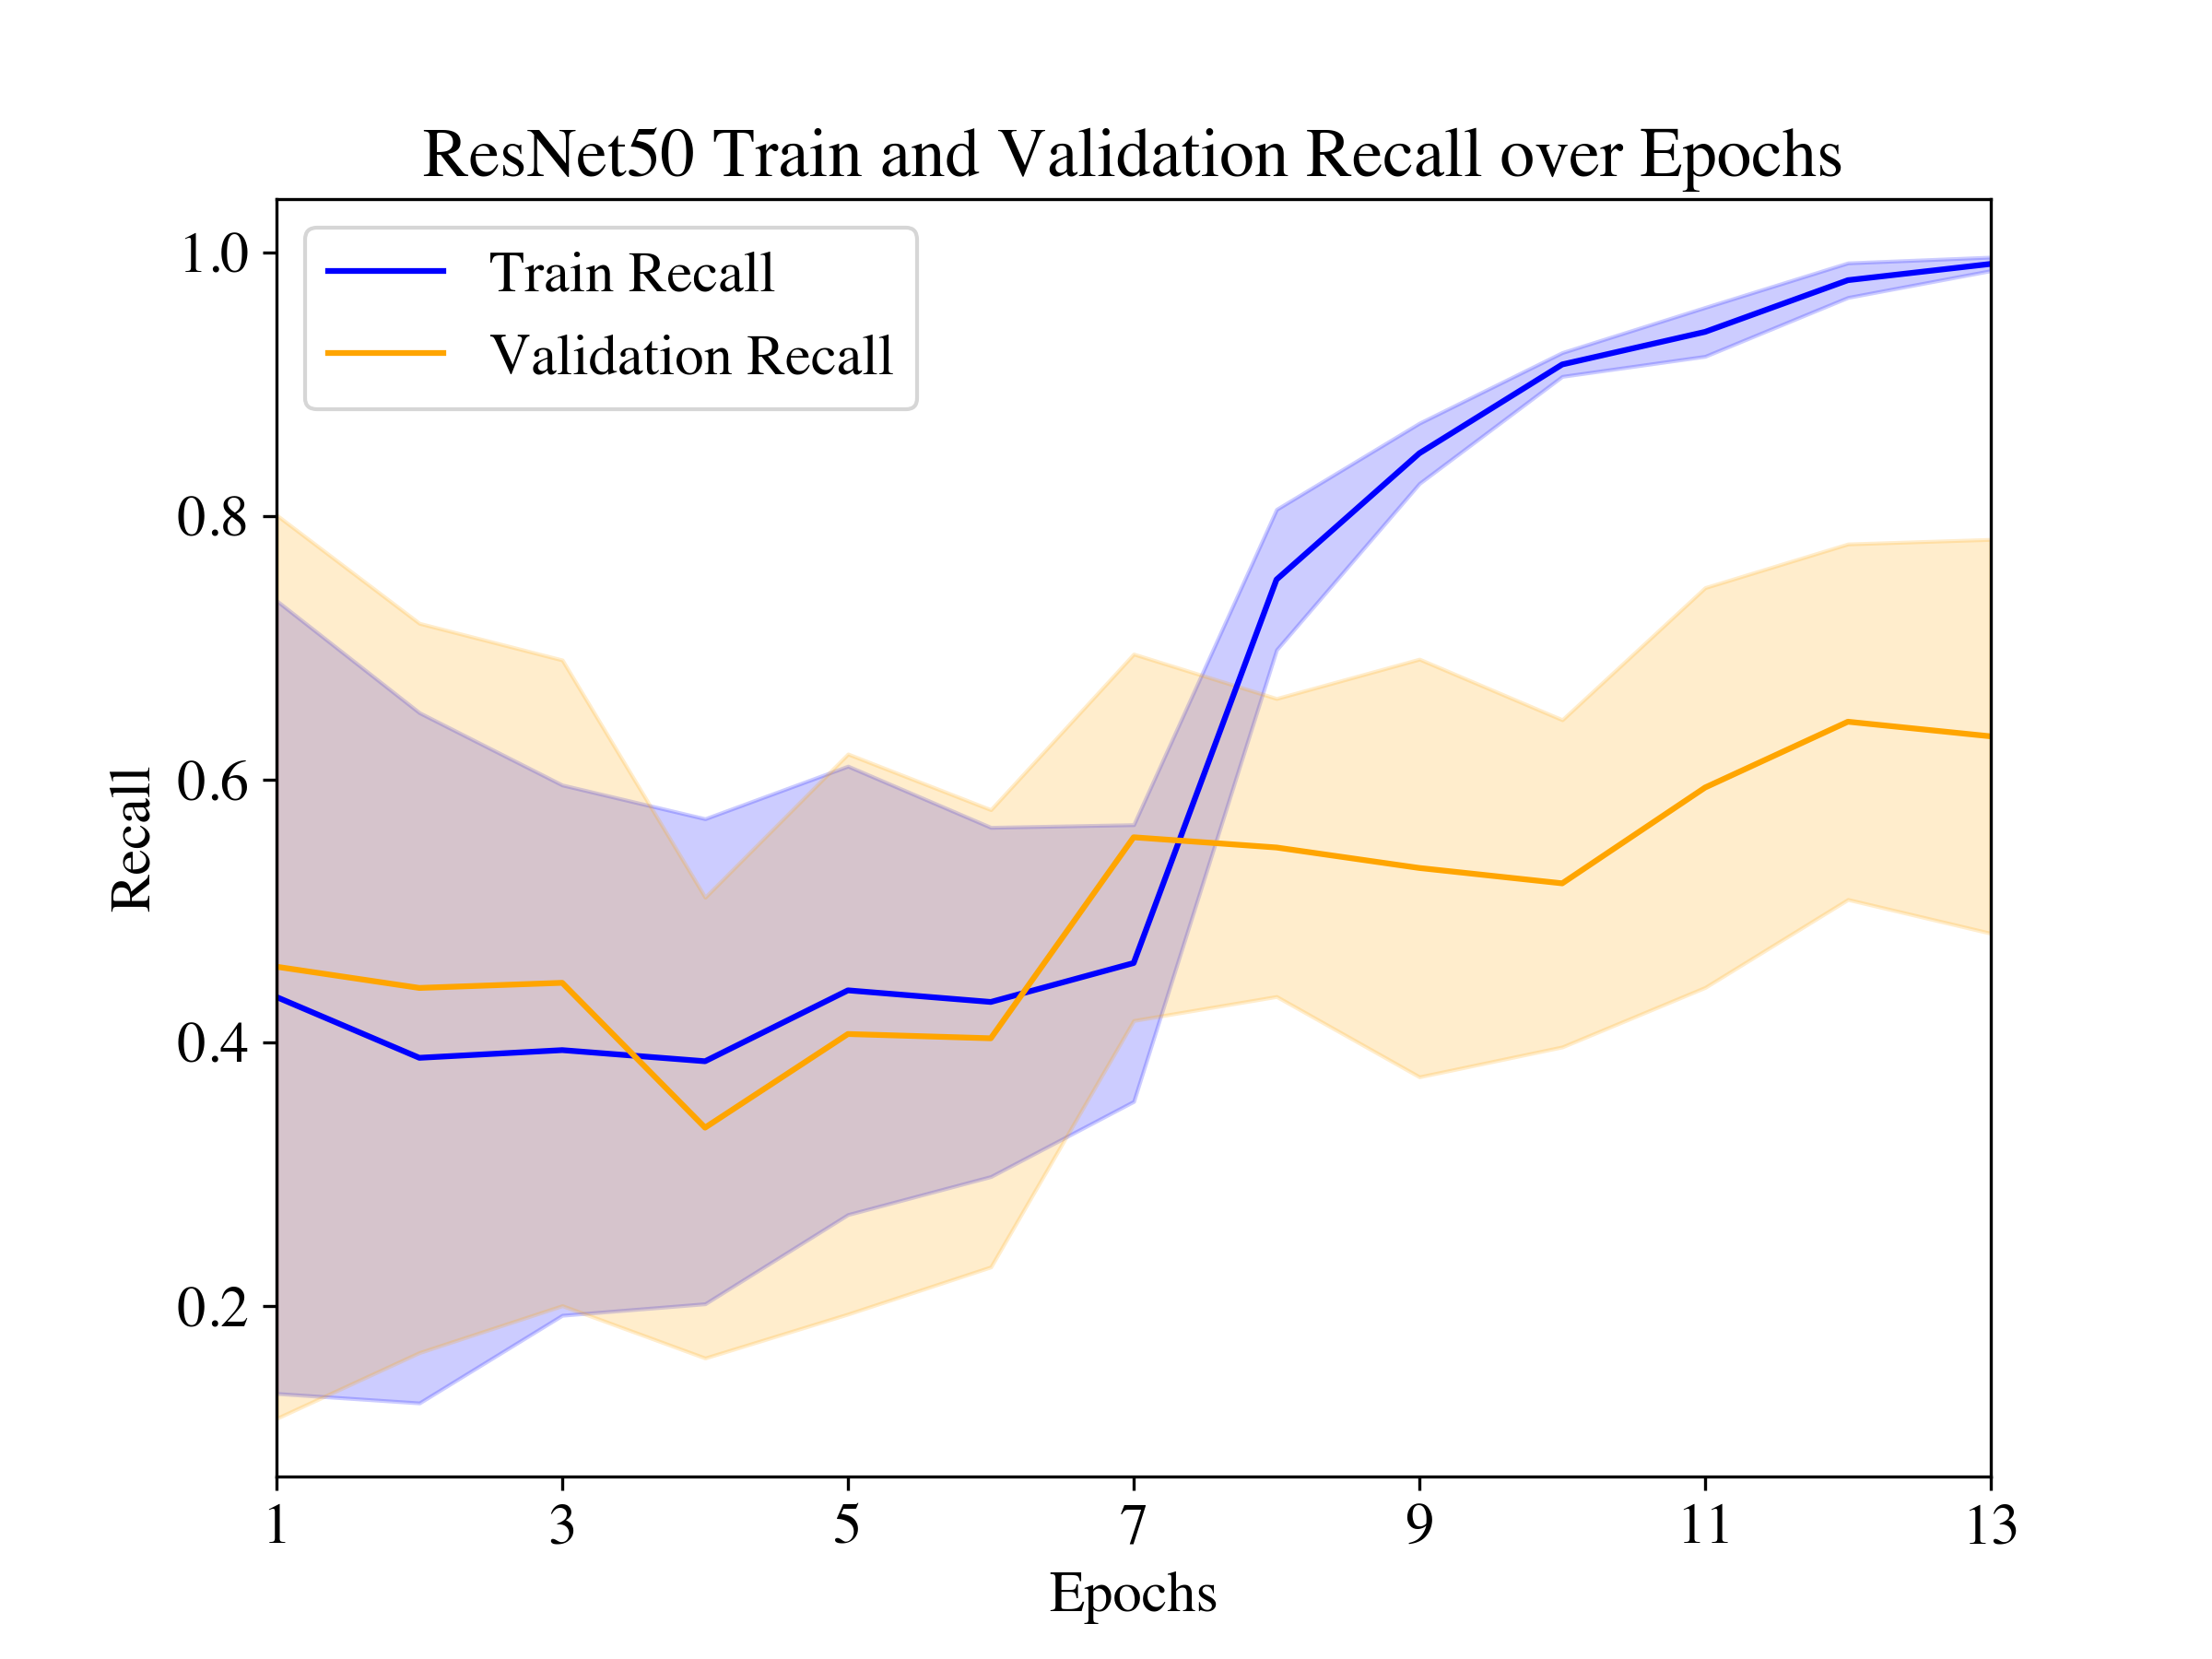
\includegraphics[width=.4\linewidth]{../3d/plots/resnet50/recall.png}
\end{center}
\caption{ResNet50 train (blue) and validation (orange) loss curve (top left), accuracy curve (top right) precision curve (bottom left) validation curve (bottom right) with mean and standard deviation. This model was trained on the concatenated Retina Layer d, r, s.}
\end{figure}


\end{document}
